% Options for packages loaded elsewhere
\PassOptionsToPackage{unicode}{hyperref}
\PassOptionsToPackage{hyphens}{url}
\PassOptionsToPackage{dvipsnames,svgnames,x11names}{xcolor}
%
\documentclass[
  letterpaper,
  DIV=11,
  numbers=noendperiod]{scrartcl}

\usepackage{amsmath,amssymb}
\usepackage{iftex}
\ifPDFTeX
  \usepackage[T1]{fontenc}
  \usepackage[utf8]{inputenc}
  \usepackage{textcomp} % provide euro and other symbols
\else % if luatex or xetex
  \usepackage{unicode-math}
  \defaultfontfeatures{Scale=MatchLowercase}
  \defaultfontfeatures[\rmfamily]{Ligatures=TeX,Scale=1}
\fi
\usepackage{lmodern}
\ifPDFTeX\else  
    % xetex/luatex font selection
\fi
% Use upquote if available, for straight quotes in verbatim environments
\IfFileExists{upquote.sty}{\usepackage{upquote}}{}
\IfFileExists{microtype.sty}{% use microtype if available
  \usepackage[]{microtype}
  \UseMicrotypeSet[protrusion]{basicmath} % disable protrusion for tt fonts
}{}
\makeatletter
\@ifundefined{KOMAClassName}{% if non-KOMA class
  \IfFileExists{parskip.sty}{%
    \usepackage{parskip}
  }{% else
    \setlength{\parindent}{0pt}
    \setlength{\parskip}{6pt plus 2pt minus 1pt}}
}{% if KOMA class
  \KOMAoptions{parskip=half}}
\makeatother
\usepackage{xcolor}
\usepackage{svg}
\setlength{\emergencystretch}{3em} % prevent overfull lines
\setcounter{secnumdepth}{5}
% Make \paragraph and \subparagraph free-standing
\makeatletter
\ifx\paragraph\undefined\else
  \let\oldparagraph\paragraph
  \renewcommand{\paragraph}{
    \@ifstar
      \xxxParagraphStar
      \xxxParagraphNoStar
  }
  \newcommand{\xxxParagraphStar}[1]{\oldparagraph*{#1}\mbox{}}
  \newcommand{\xxxParagraphNoStar}[1]{\oldparagraph{#1}\mbox{}}
\fi
\ifx\subparagraph\undefined\else
  \let\oldsubparagraph\subparagraph
  \renewcommand{\subparagraph}{
    \@ifstar
      \xxxSubParagraphStar
      \xxxSubParagraphNoStar
  }
  \newcommand{\xxxSubParagraphStar}[1]{\oldsubparagraph*{#1}\mbox{}}
  \newcommand{\xxxSubParagraphNoStar}[1]{\oldsubparagraph{#1}\mbox{}}
\fi
\makeatother

\usepackage{color}
\usepackage{fancyvrb}
\newcommand{\VerbBar}{|}
\newcommand{\VERB}{\Verb[commandchars=\\\{\}]}
\DefineVerbatimEnvironment{Highlighting}{Verbatim}{commandchars=\\\{\}}
% Add ',fontsize=\small' for more characters per line
\usepackage{framed}
\definecolor{shadecolor}{RGB}{241,243,245}
\newenvironment{Shaded}{\begin{snugshade}}{\end{snugshade}}
\newcommand{\AlertTok}[1]{\textcolor[rgb]{0.68,0.00,0.00}{#1}}
\newcommand{\AnnotationTok}[1]{\textcolor[rgb]{0.37,0.37,0.37}{#1}}
\newcommand{\AttributeTok}[1]{\textcolor[rgb]{0.40,0.45,0.13}{#1}}
\newcommand{\BaseNTok}[1]{\textcolor[rgb]{0.68,0.00,0.00}{#1}}
\newcommand{\BuiltInTok}[1]{\textcolor[rgb]{0.00,0.23,0.31}{#1}}
\newcommand{\CharTok}[1]{\textcolor[rgb]{0.13,0.47,0.30}{#1}}
\newcommand{\CommentTok}[1]{\textcolor[rgb]{0.37,0.37,0.37}{#1}}
\newcommand{\CommentVarTok}[1]{\textcolor[rgb]{0.37,0.37,0.37}{\textit{#1}}}
\newcommand{\ConstantTok}[1]{\textcolor[rgb]{0.56,0.35,0.01}{#1}}
\newcommand{\ControlFlowTok}[1]{\textcolor[rgb]{0.00,0.23,0.31}{\textbf{#1}}}
\newcommand{\DataTypeTok}[1]{\textcolor[rgb]{0.68,0.00,0.00}{#1}}
\newcommand{\DecValTok}[1]{\textcolor[rgb]{0.68,0.00,0.00}{#1}}
\newcommand{\DocumentationTok}[1]{\textcolor[rgb]{0.37,0.37,0.37}{\textit{#1}}}
\newcommand{\ErrorTok}[1]{\textcolor[rgb]{0.68,0.00,0.00}{#1}}
\newcommand{\ExtensionTok}[1]{\textcolor[rgb]{0.00,0.23,0.31}{#1}}
\newcommand{\FloatTok}[1]{\textcolor[rgb]{0.68,0.00,0.00}{#1}}
\newcommand{\FunctionTok}[1]{\textcolor[rgb]{0.28,0.35,0.67}{#1}}
\newcommand{\ImportTok}[1]{\textcolor[rgb]{0.00,0.46,0.62}{#1}}
\newcommand{\InformationTok}[1]{\textcolor[rgb]{0.37,0.37,0.37}{#1}}
\newcommand{\KeywordTok}[1]{\textcolor[rgb]{0.00,0.23,0.31}{\textbf{#1}}}
\newcommand{\NormalTok}[1]{\textcolor[rgb]{0.00,0.23,0.31}{#1}}
\newcommand{\OperatorTok}[1]{\textcolor[rgb]{0.37,0.37,0.37}{#1}}
\newcommand{\OtherTok}[1]{\textcolor[rgb]{0.00,0.23,0.31}{#1}}
\newcommand{\PreprocessorTok}[1]{\textcolor[rgb]{0.68,0.00,0.00}{#1}}
\newcommand{\RegionMarkerTok}[1]{\textcolor[rgb]{0.00,0.23,0.31}{#1}}
\newcommand{\SpecialCharTok}[1]{\textcolor[rgb]{0.37,0.37,0.37}{#1}}
\newcommand{\SpecialStringTok}[1]{\textcolor[rgb]{0.13,0.47,0.30}{#1}}
\newcommand{\StringTok}[1]{\textcolor[rgb]{0.13,0.47,0.30}{#1}}
\newcommand{\VariableTok}[1]{\textcolor[rgb]{0.07,0.07,0.07}{#1}}
\newcommand{\VerbatimStringTok}[1]{\textcolor[rgb]{0.13,0.47,0.30}{#1}}
\newcommand{\WarningTok}[1]{\textcolor[rgb]{0.37,0.37,0.37}{\textit{#1}}}

\providecommand{\tightlist}{%
  \setlength{\itemsep}{0pt}\setlength{\parskip}{0pt}}\usepackage{longtable,booktabs,array}
\usepackage{calc} % for calculating minipage widths
% Correct order of tables after \paragraph or \subparagraph
\usepackage{etoolbox}
\makeatletter
\patchcmd\longtable{\par}{\if@noskipsec\mbox{}\fi\par}{}{}
\makeatother
% Allow footnotes in longtable head/foot
\IfFileExists{footnotehyper.sty}{\usepackage{footnotehyper}}{\usepackage{footnote}}
\makesavenoteenv{longtable}
\usepackage{graphicx}
\makeatletter
\newsavebox\pandoc@box
\newcommand*\pandocbounded[1]{% scales image to fit in text height/width
  \sbox\pandoc@box{#1}%
  \Gscale@div\@tempa{\textheight}{\dimexpr\ht\pandoc@box+\dp\pandoc@box\relax}%
  \Gscale@div\@tempb{\linewidth}{\wd\pandoc@box}%
  \ifdim\@tempb\p@<\@tempa\p@\let\@tempa\@tempb\fi% select the smaller of both
  \ifdim\@tempa\p@<\p@\scalebox{\@tempa}{\usebox\pandoc@box}%
  \else\usebox{\pandoc@box}%
  \fi%
}
% Set default figure placement to htbp
\def\fps@figure{htbp}
\makeatother

\KOMAoption{captions}{tableheading}
\makeatletter
\@ifpackageloaded{tcolorbox}{}{\usepackage[skins,breakable]{tcolorbox}}
\@ifpackageloaded{fontawesome5}{}{\usepackage{fontawesome5}}
\definecolor{quarto-callout-color}{HTML}{909090}
\definecolor{quarto-callout-note-color}{HTML}{0758E5}
\definecolor{quarto-callout-important-color}{HTML}{CC1914}
\definecolor{quarto-callout-warning-color}{HTML}{EB9113}
\definecolor{quarto-callout-tip-color}{HTML}{00A047}
\definecolor{quarto-callout-caution-color}{HTML}{FC5300}
\definecolor{quarto-callout-color-frame}{HTML}{acacac}
\definecolor{quarto-callout-note-color-frame}{HTML}{4582ec}
\definecolor{quarto-callout-important-color-frame}{HTML}{d9534f}
\definecolor{quarto-callout-warning-color-frame}{HTML}{f0ad4e}
\definecolor{quarto-callout-tip-color-frame}{HTML}{02b875}
\definecolor{quarto-callout-caution-color-frame}{HTML}{fd7e14}
\makeatother
\makeatletter
\@ifpackageloaded{caption}{}{\usepackage{caption}}
\AtBeginDocument{%
\ifdefined\contentsname
  \renewcommand*\contentsname{Table of contents}
\else
  \newcommand\contentsname{Table of contents}
\fi
\ifdefined\listfigurename
  \renewcommand*\listfigurename{List of Figures}
\else
  \newcommand\listfigurename{List of Figures}
\fi
\ifdefined\listtablename
  \renewcommand*\listtablename{List of Tables}
\else
  \newcommand\listtablename{List of Tables}
\fi
\ifdefined\figurename
  \renewcommand*\figurename{Figure}
\else
  \newcommand\figurename{Figure}
\fi
\ifdefined\tablename
  \renewcommand*\tablename{Table}
\else
  \newcommand\tablename{Table}
\fi
}
\@ifpackageloaded{float}{}{\usepackage{float}}
\floatstyle{ruled}
\@ifundefined{c@chapter}{\newfloat{codelisting}{h}{lop}}{\newfloat{codelisting}{h}{lop}[chapter]}
\floatname{codelisting}{Listing}
\newcommand*\listoflistings{\listof{codelisting}{List of Listings}}
\makeatother
\makeatletter
\makeatother
\makeatletter
\@ifpackageloaded{caption}{}{\usepackage{caption}}
\@ifpackageloaded{subcaption}{}{\usepackage{subcaption}}
\makeatother

\usepackage{bookmark}

\IfFileExists{xurl.sty}{\usepackage{xurl}}{} % add URL line breaks if available
\urlstyle{same} % disable monospaced font for URLs
\hypersetup{
  pdftitle={Using Open Geospatial Data in GIS},
  pdfauthor={Felipe Valdez},
  colorlinks=true,
  linkcolor={blue},
  filecolor={Maroon},
  citecolor={Blue},
  urlcolor={Blue},
  pdfcreator={LaTeX via pandoc}}


\title{Using Open Geospatial Data in GIS}
\author{Felipe Valdez}
\date{}

\begin{document}
\maketitle

\renewcommand*\contentsname{Contents}
{
\hypersetup{linkcolor=}
\setcounter{tocdepth}{4}
\tableofcontents
}

\section{Why Open Geospatial Data?}\label{why-open-geospatial-data}

In the world of data, \texttt{open} means different things. First, it's
about who can access and use the data. Second, it's about how that data
can be used - from the transparency of its creation and handling to the
standards and protocols that make the data accessible.

Thanks to advances in computing and the internet, many organizations now
embrace open data policies to share, access, and create value from data.

Having an open data policy offers several key benefits:

\begin{itemize}
\item
  Greater transparency, especially for governments. When data is open,
  citizens can see and understand what their government is doing.
\item
  Increased public participation. Open data allows citizens to engage
  with and contribute to solutions for their communities.
\item
  Faster and more significant advances in knowledge. Instead of spending
  time and money generating new data, researchers can build on existing
  information.
\item
  Better reproducibility of research results. Other scientists can
  verify and build upon previous work.
\item
  Improved informed decision-making, particularly for global-scale
  problems. When decision-makers have access to good data, they make
  better choices.
\end{itemize}

Open geospatial data is especially crucial for tackling global
challenges like climate change, urban development, and disaster
response. In these situations, quick access to accurate location-based
information can make the difference in coordinating effective responses
and making smart decisions.

\section{Sources reviewed in this
tutorial}\label{sources-reviewed-in-this-tutorial}

In this guide, we'll explore ways to access and use open geospatial
data, focusing on OpenStreetMap and Overture Maps for Geographic
Information Systems (QGIS specifically). These tools are powerful
resources that anyone can use to work with location-based data.

\subsection{OpenStreetMap OSM}\label{openstreetmap-osm}

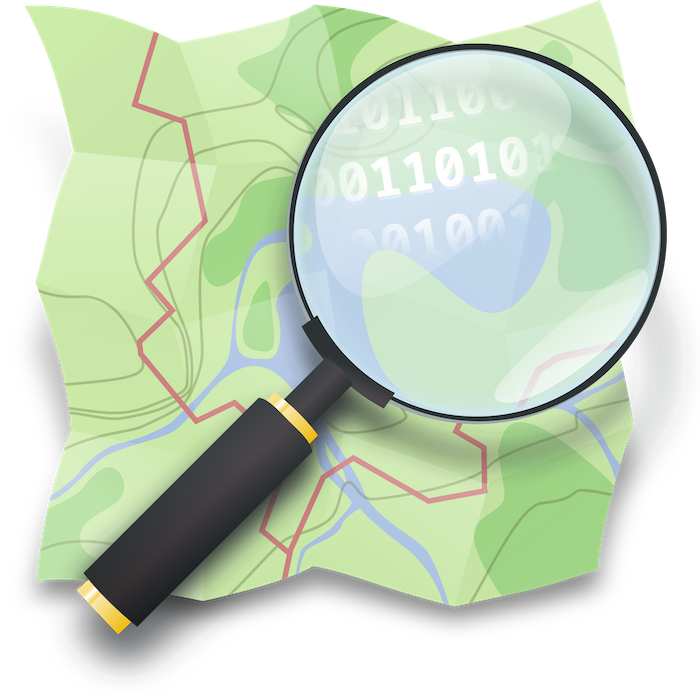
\includegraphics[width=1.5625in,height=\textheight,keepaspectratio]{./images/osmlogo.png}

\href{openstreemap.org}{OpenStreetMap} (OSM) is a collaborative world
map that anyone can edit and use - think of it like ``Wikipedia for
maps.'' It is created by volunteers worldwide who add and update
geographic information about roads, buildings, parks, businesses, and
other features. People contribute data based on their local knowledge,
GPS tracks, aerial imagery, and field surveys.

Key aspects of OSM:

\begin{itemize}
\item
  \textbf{Community-driven:} The data is collected and maintained by a
  global community of mappers, from hobbyists to professional
  geographers.
\item
  \textbf{Truly open:} Unlike commercial maps, OSM data is freely
  available for anyone to download, use, and modify under an open
  license (Open Database License).
\item
  \textbf{Used everywhere:} The data powers thousands of applications
  and services - from humanitarian crisis response to navigation apps,
  urban planning tools, and games.
\item
  \textbf{Constantly updated:} Because anyone can contribute, OSM often
  has more up-to-date information than commercial maps, especially in
  rapidly changing areas or after natural disasters.
\end{itemize}

These are only some of the communities building OSM. Explore more
communities \href{https://www.openstreetmap.org/communities}{here}

\pandocbounded{
\includegraphics[keepaspectratio]{./images/commosm.png}}

The project started in 2004 in the UK and has grown into one of the
largest collaborative mapping efforts in the world. Today, OSM is often
considered the most comprehensive free source of geographic data
available.

Although you don't need an account to explore the map, you can
\href{https://www.openstreetmap.org/user/new}{sign up} if you want to
contribute edits or be part of the communities related to the project.

\pandocbounded{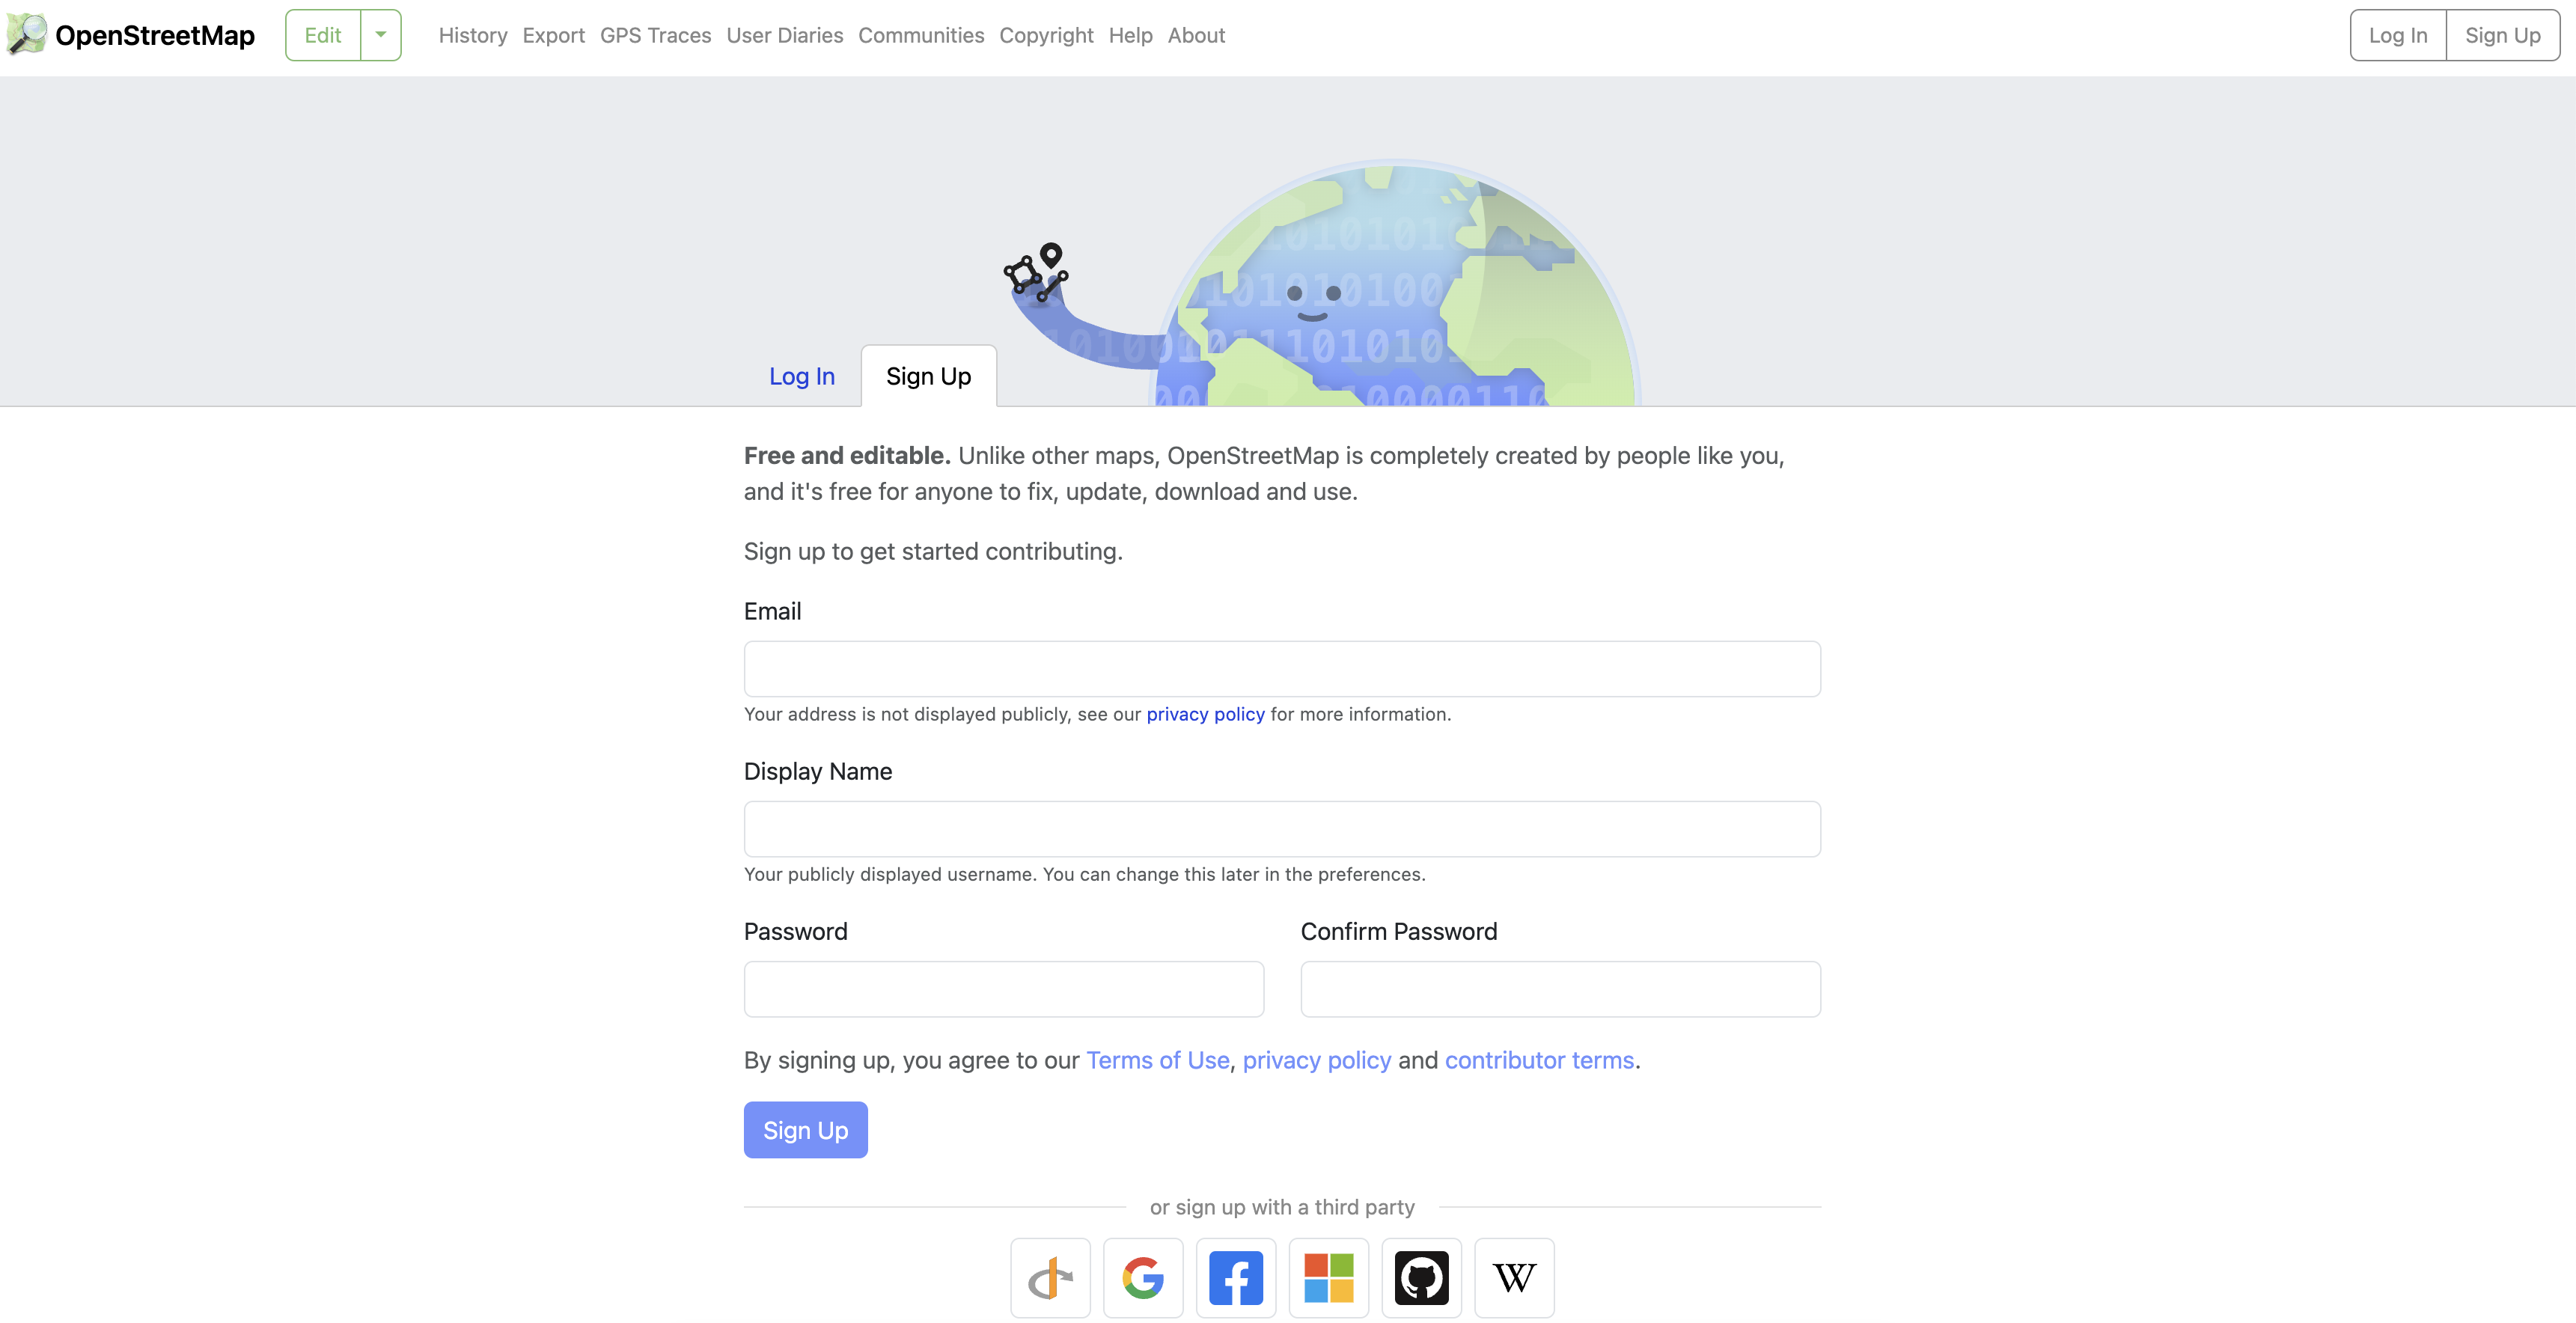
\includegraphics[keepaspectratio]{./images/signuposm.png}}

\subsection{Overture Maps}\label{overture-maps}


\includegraphics[width=3.125in,height=\textheight,keepaspectratio]{./images/overturelogo.png}

\href{https://overturemaps.org/}{Overture Maps} is a newer collaborative
effort launched in 2022 by major tech companies including Meta,
Microsoft, Amazon (AWS), and TomTom. It combines information from
multiple sources - including commercial datasets, open data, and machine
learning - to create a high-quality, standardized global map.

Key aspects of Overture Maps:

\begin{itemize}
\item
  \textbf{Quality-focused:} It uses sophisticated data validation and
  conflation techniques to ensure accuracy and consistency of geographic
  information.
\item
  \textbf{Business-friendly:} While free and open like OSM, it's
  specifically designed to meet enterprise-level mapping needs with
  reliable, standardized data.
\item
  \textbf{Modern architecture:} Built from the ground up to handle
  today's mapping challenges, with a focus on regular updates and clear
  data lineage.
\item
  \textbf{Multiple sources:} Instead of relying solely on volunteer
  contributions, it combines different data sources including commercial
  data, open data, and machine-derived features.
\end{itemize}

The project released its first major dataset in 2023 and aims to provide
an alternative foundation for building mapping applications and
services. While newer than OSM, it's designed to complement rather than
compete with existing open mapping projects.

\section{Exploring the data}\label{exploring-the-data}

\subsection{In OpenStreetMap}\label{in-openstreetmap}

{01} \emph{Go to \url{https://www.openstreetmap.org/} on your web
browser}

\pandocbounded{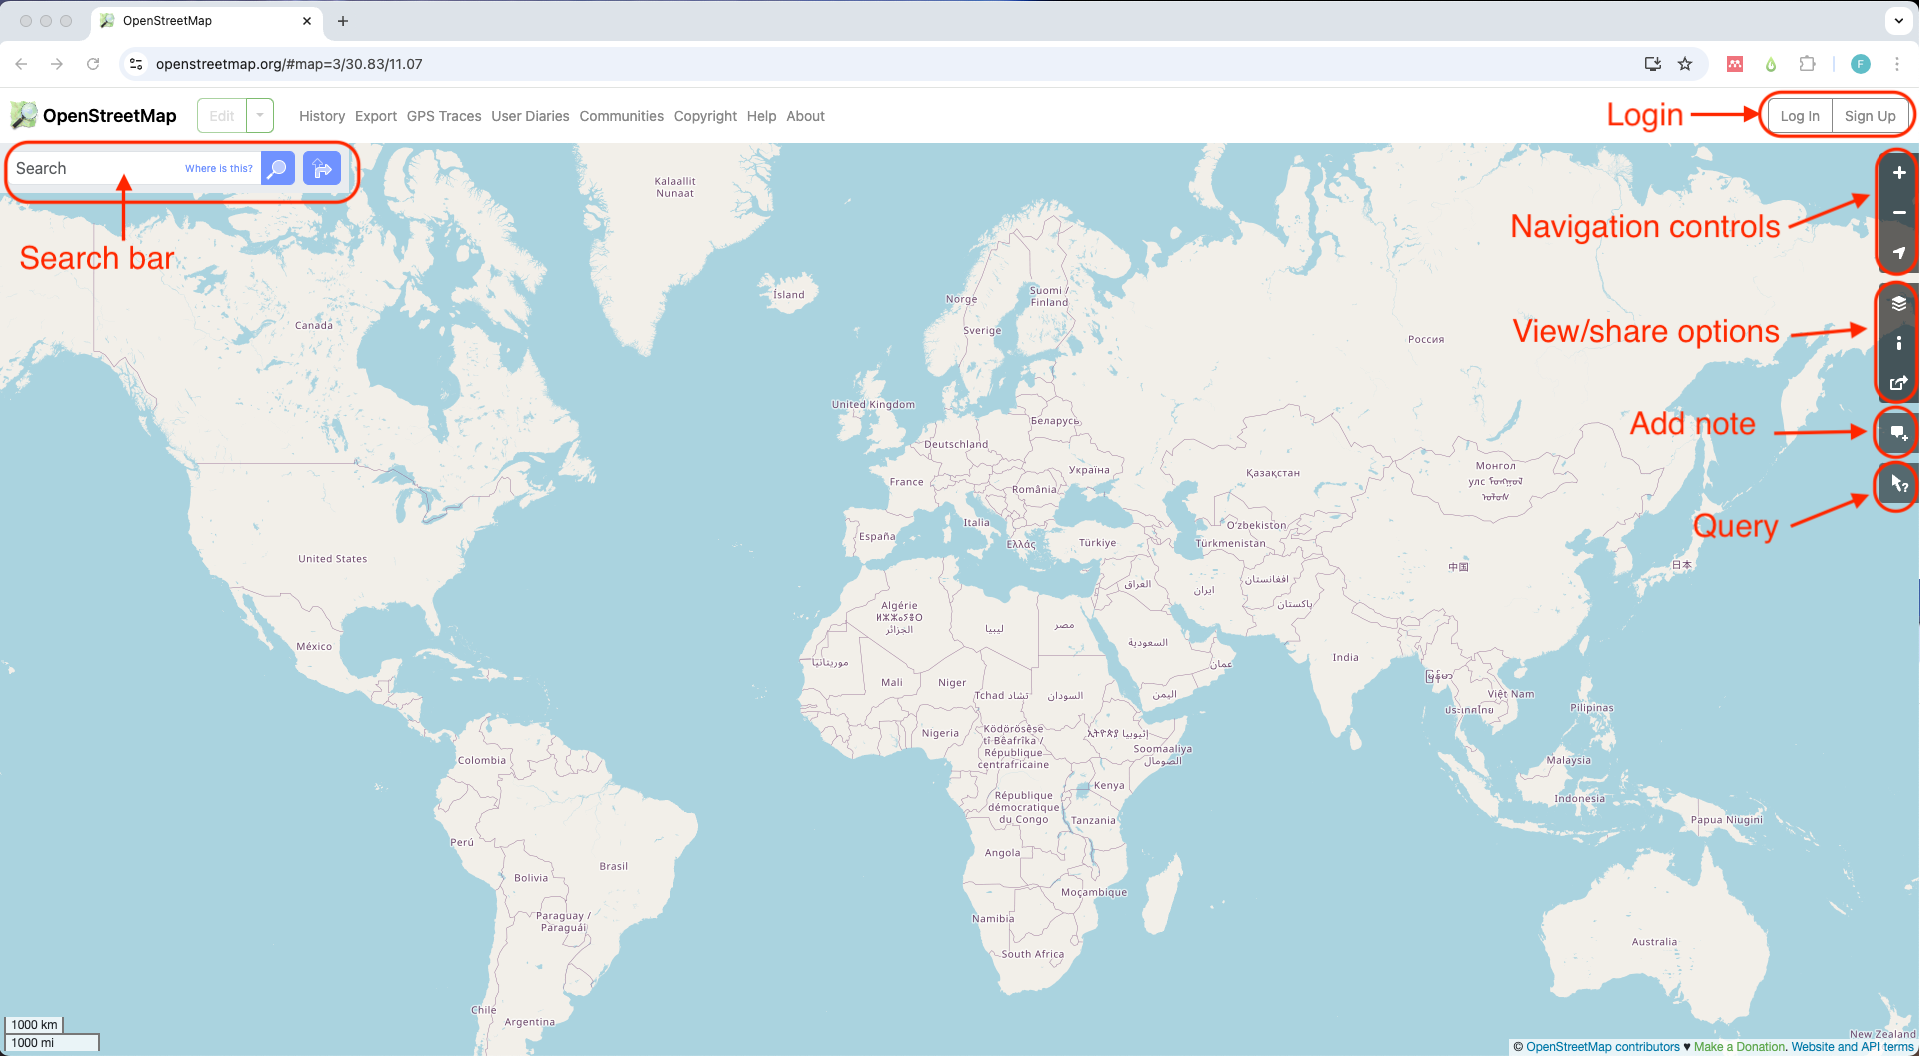
\includegraphics[keepaspectratio]{./images/osm_tools.png}}

The screen will show a big area with a map on the center. To explore the
map you can use the \texttt{Search} bar located on the top left corner.
Simply type the name of a place or a street address and click
\texttt{enter/return} or the search icon. You can also use the
\texttt{Navigation\ controls} (zoom in +/zoom out -/show my location)
located on the top right corner of the map.

{02} \emph{Type the name of a place in the search bar.}

When you type the name of a place in the \texttt{Search} bar, OSM will
show you a list of options found in \texttt{Nominatim}.

\begin{tcolorbox}[enhanced jigsaw, opacitybacktitle=0.6, colframe=quarto-callout-note-color-frame, arc=.35mm, leftrule=.75mm, toptitle=1mm, opacityback=0, titlerule=0mm, breakable, colback=white, colbacktitle=quarto-callout-note-color!10!white, toprule=.15mm, bottomtitle=1mm, coltitle=black, title=\textcolor{quarto-callout-note-color}{\faInfo}\hspace{0.5em}{Note}, left=2mm, rightrule=.15mm, bottomrule=.15mm]

\href{https://nominatim.org/}{\textbf{Nominatim}} is an open-source
geocoding software used to find addresses and places in OSM.

\end{tcolorbox}

Here we typed \texttt{Philadelphia} and we get six main results: the
city of Philadelphia, Pennsylvania, the county with the same name, a
town named Philadelphia in Mississippi and three other villages named
like that in other states. Notice the map has zoomed in to the city of
Philadelphia, PA. The results you get are based on the current view of
your map. If you want to see more results you can click on the button
\texttt{More\ results}.

\pandocbounded{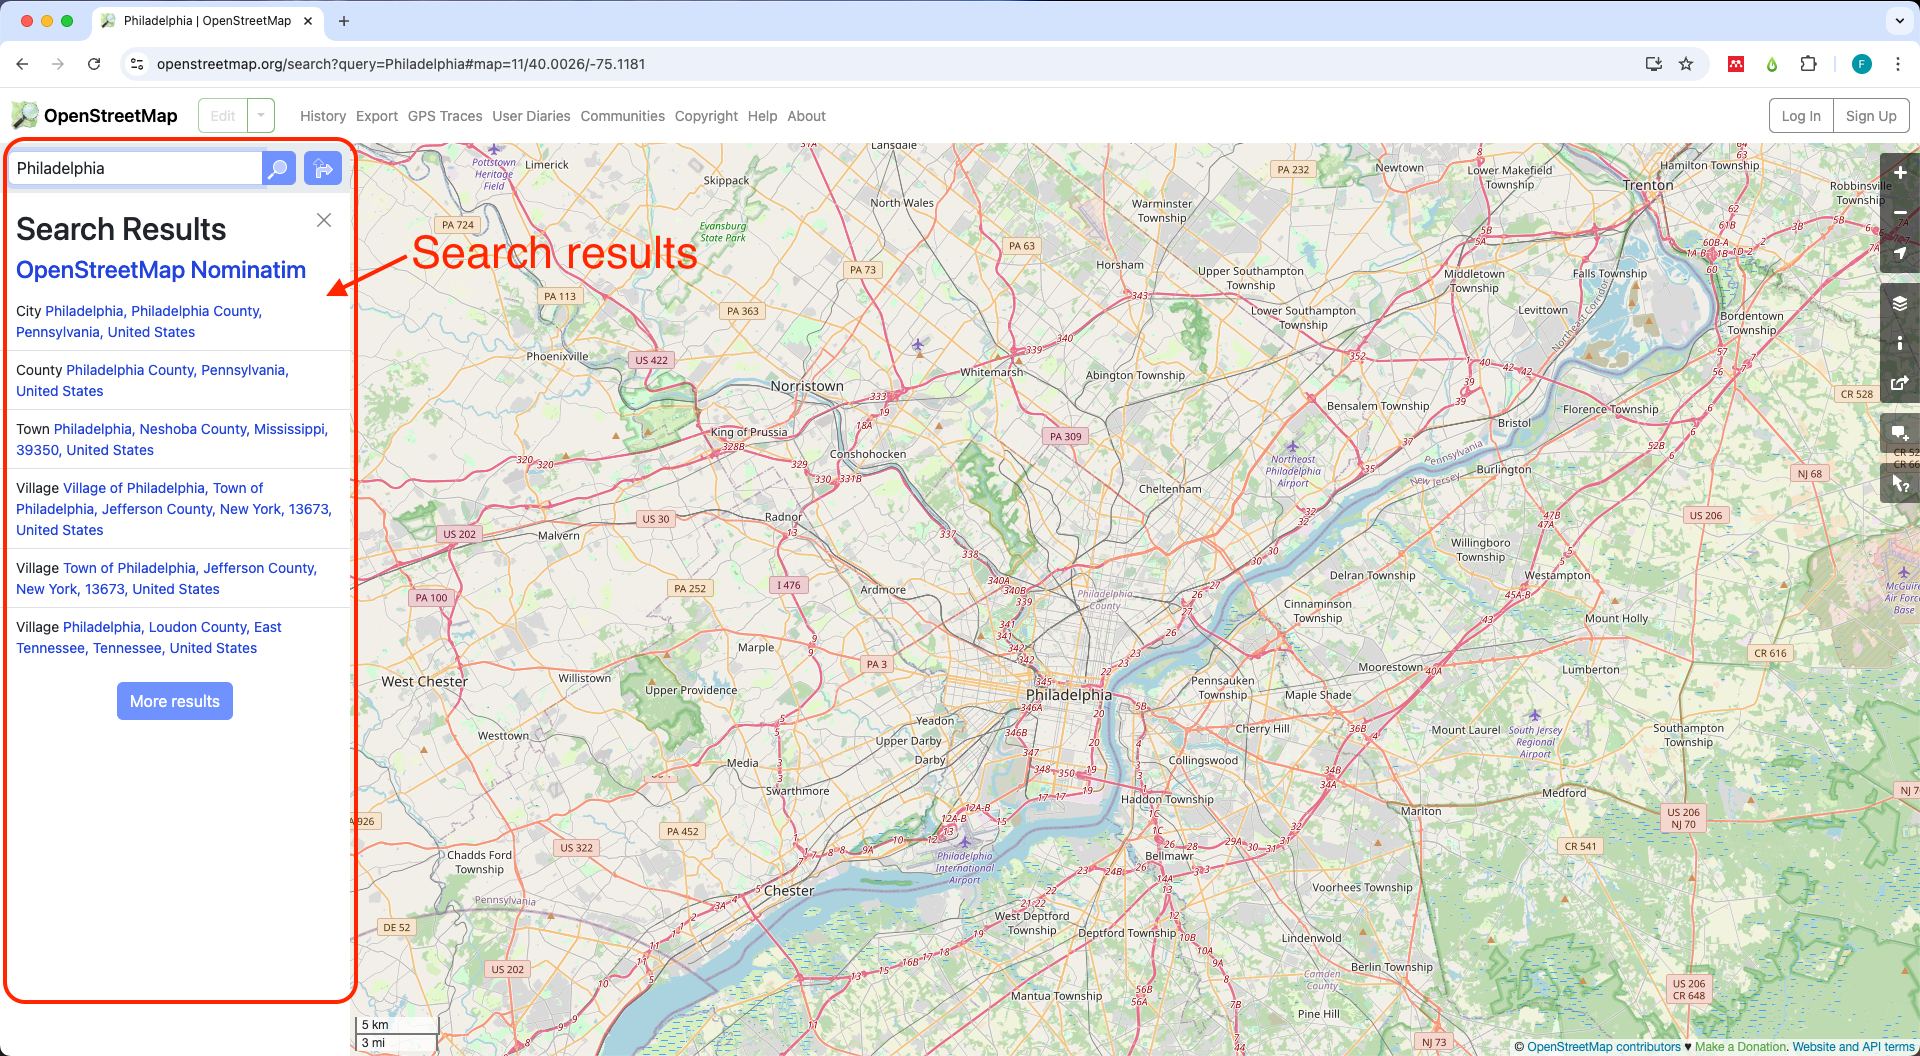
\includegraphics[keepaspectratio]{./images/search_osm.png}}

{03} \emph{Click on the result you want to explore.}

When you click on a result, the left panel will show the selected
element info and tags. On the map, you would see the element highlighted
in orange.

\pandocbounded{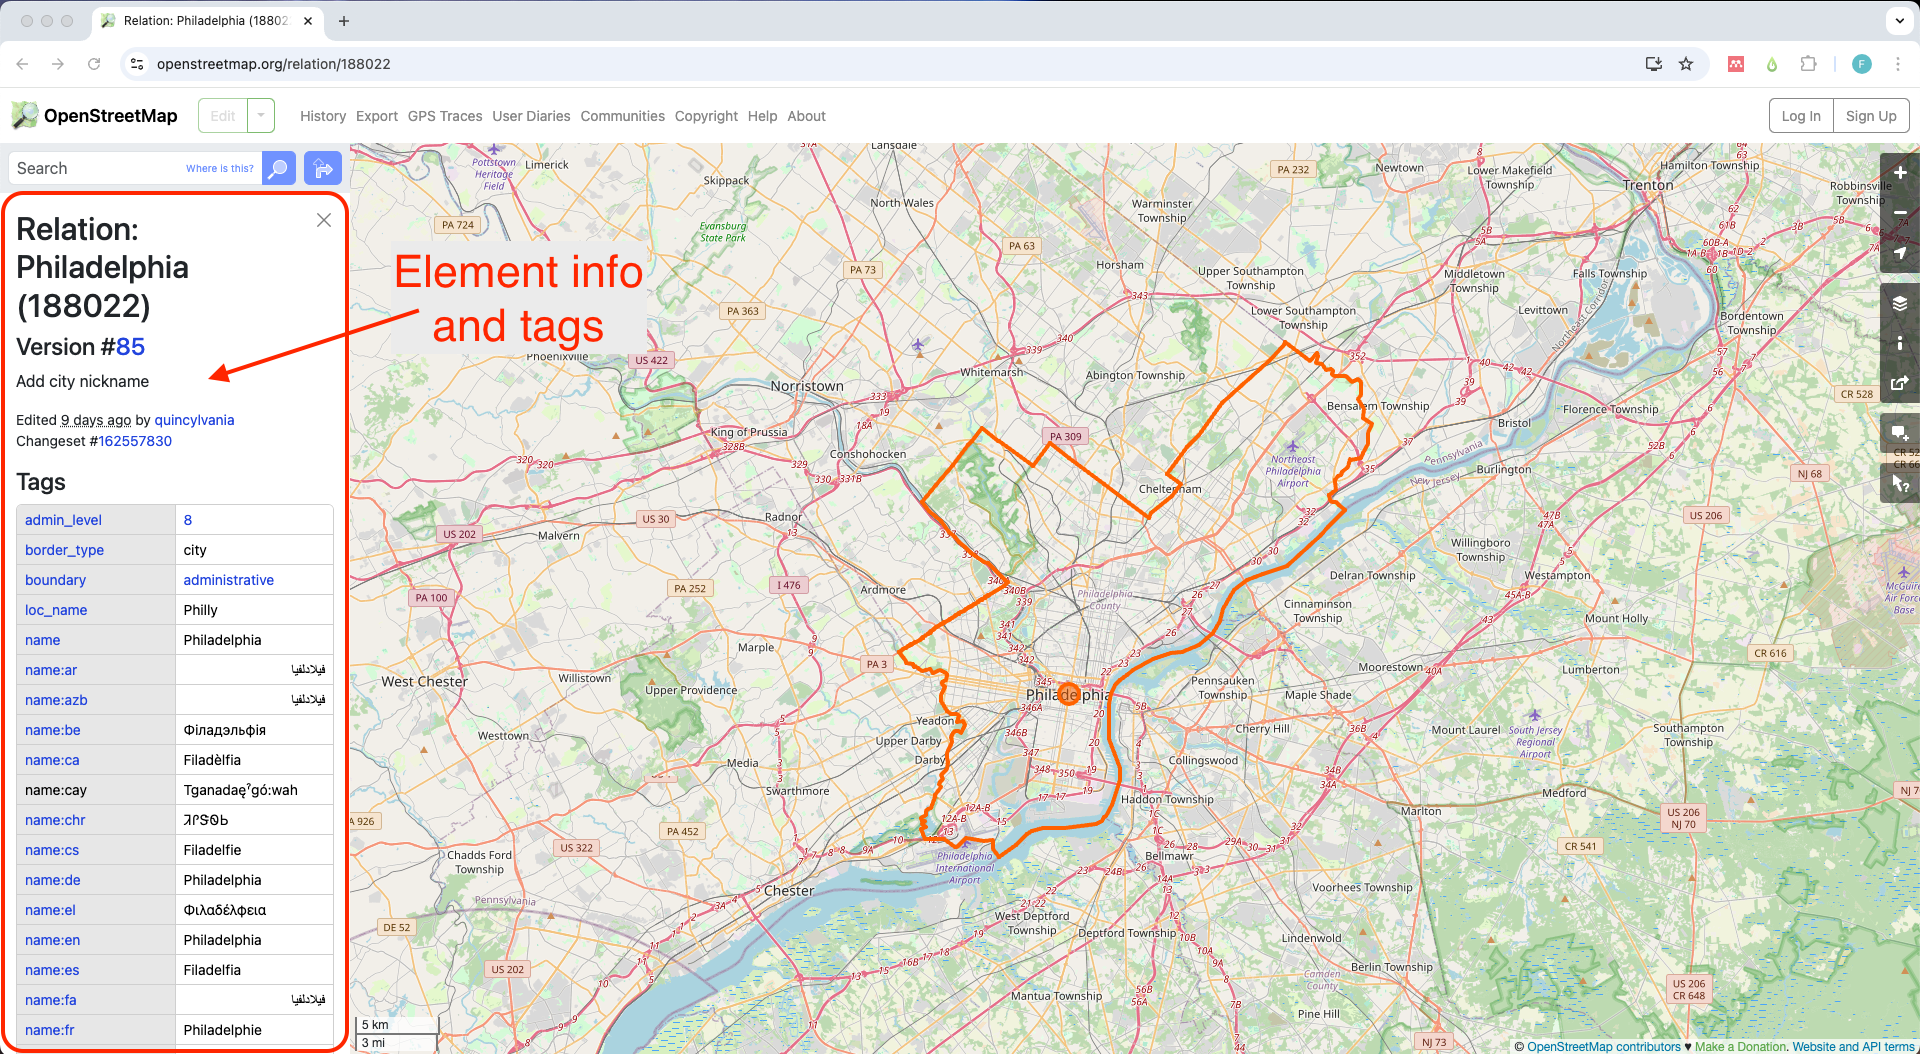
\includegraphics[keepaspectratio]{./images/element1.png}}

In this example we see an area highlighted in orange that corresponds to
the city of Philadelphia along with a node in the center of this area.
On the left side panel we see a list with all the tags assigned to this
element. For example: \texttt{border\_type:city},
\texttt{boundary:administrative}, and \texttt{loc\_name:Philly}.

\begin{tcolorbox}[enhanced jigsaw, opacitybacktitle=0.6, colframe=quarto-callout-caution-color-frame, arc=.35mm, leftrule=.75mm, toptitle=1mm, opacityback=0, titlerule=0mm, breakable, colback=white, colbacktitle=quarto-callout-caution-color!10!white, toprule=.15mm, bottomtitle=1mm, coltitle=black, title=\textcolor{quarto-callout-caution-color}{\faFire}\hspace{0.5em}{How data is organized in OSM?}, left=2mm, rightrule=.15mm, bottomrule=.15mm]

All data in OSM is represented by an \textbf{element.}

An \textbf{element} can be either a \texttt{node}
\includesvg[width=0.03\linewidth,height=\textheight,keepaspectratio]{opengeodata_files/mediabag/Osm_element_node.svg},
a \texttt{way}
\includesvg[width=0.03\linewidth,height=\textheight,keepaspectratio]{opengeodata_files/mediabag/Osm_element_way.svg}
or a \texttt{relation}
\includesvg[width=0.03\linewidth,height=\textheight,keepaspectratio]{opengeodata_files/mediabag/Osm_element_relation.svg}.

Each element is described using \texttt{tags} which are the combination
of a \texttt{key} and a \texttt{value}
\includesvg[width=0.3125in,height=0.3125in]{opengeodata_files/mediabag/Mf_tag.svg}.
For example, a coffee shop is represented by an element type
\texttt{node} with tags \texttt{amenity=cafe}.

Learn more about elements and tags
\href{https://wiki.openstreetmap.org/wiki/Elements}{here.}

\end{tcolorbox}

\subsubsection{Querying the data}\label{querying-the-data}

Now lets query the data we see on the map to discover the type of
element and what tags are being used to describe it.

{04} \emph{Type the name of a place in the search bar.}

We are going to explore a more local area by typing
\texttt{charles\ library,\ philadelphia} in the search bar. This will
zoom in the map further.

\pandocbounded{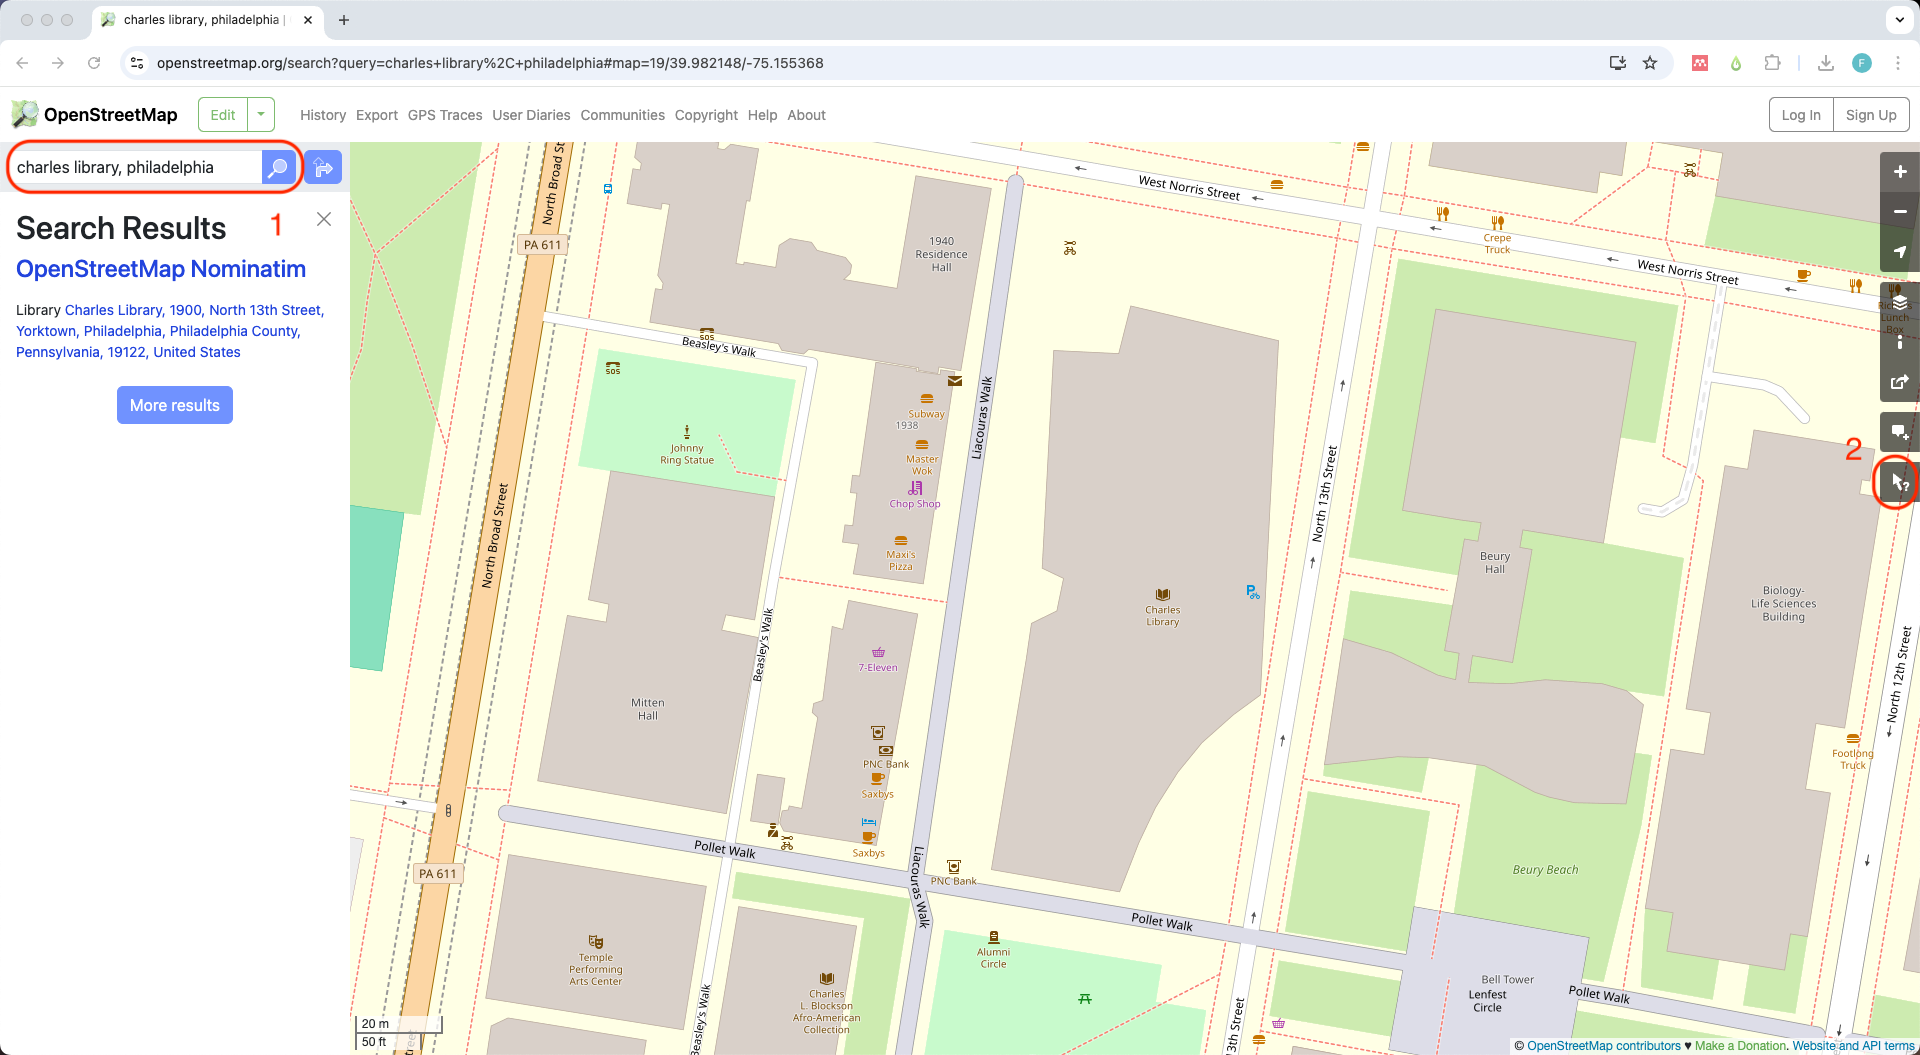
\includegraphics[keepaspectratio]{./images/charlesosm.png}}

{05} \emph{Click on the `Query features' tool.}

On the right side of the screen, click on the \texttt{Query\ features}
tool
\pandocbounded{
\includegraphics[keepaspectratio]{./images/queryosm.png}}

You will notice the mouse cursor icon will change to a question mark.

{06} \emph{Click on any element you see on the map to query.}

Now, if you click on any area of the map, the left side panel will show
two lists: `Nearby features' and `Enclosing features'. The Nearby
feaures list will have all elements close to the point you clicked on
the map. In this example, we got seven results.

\pandocbounded{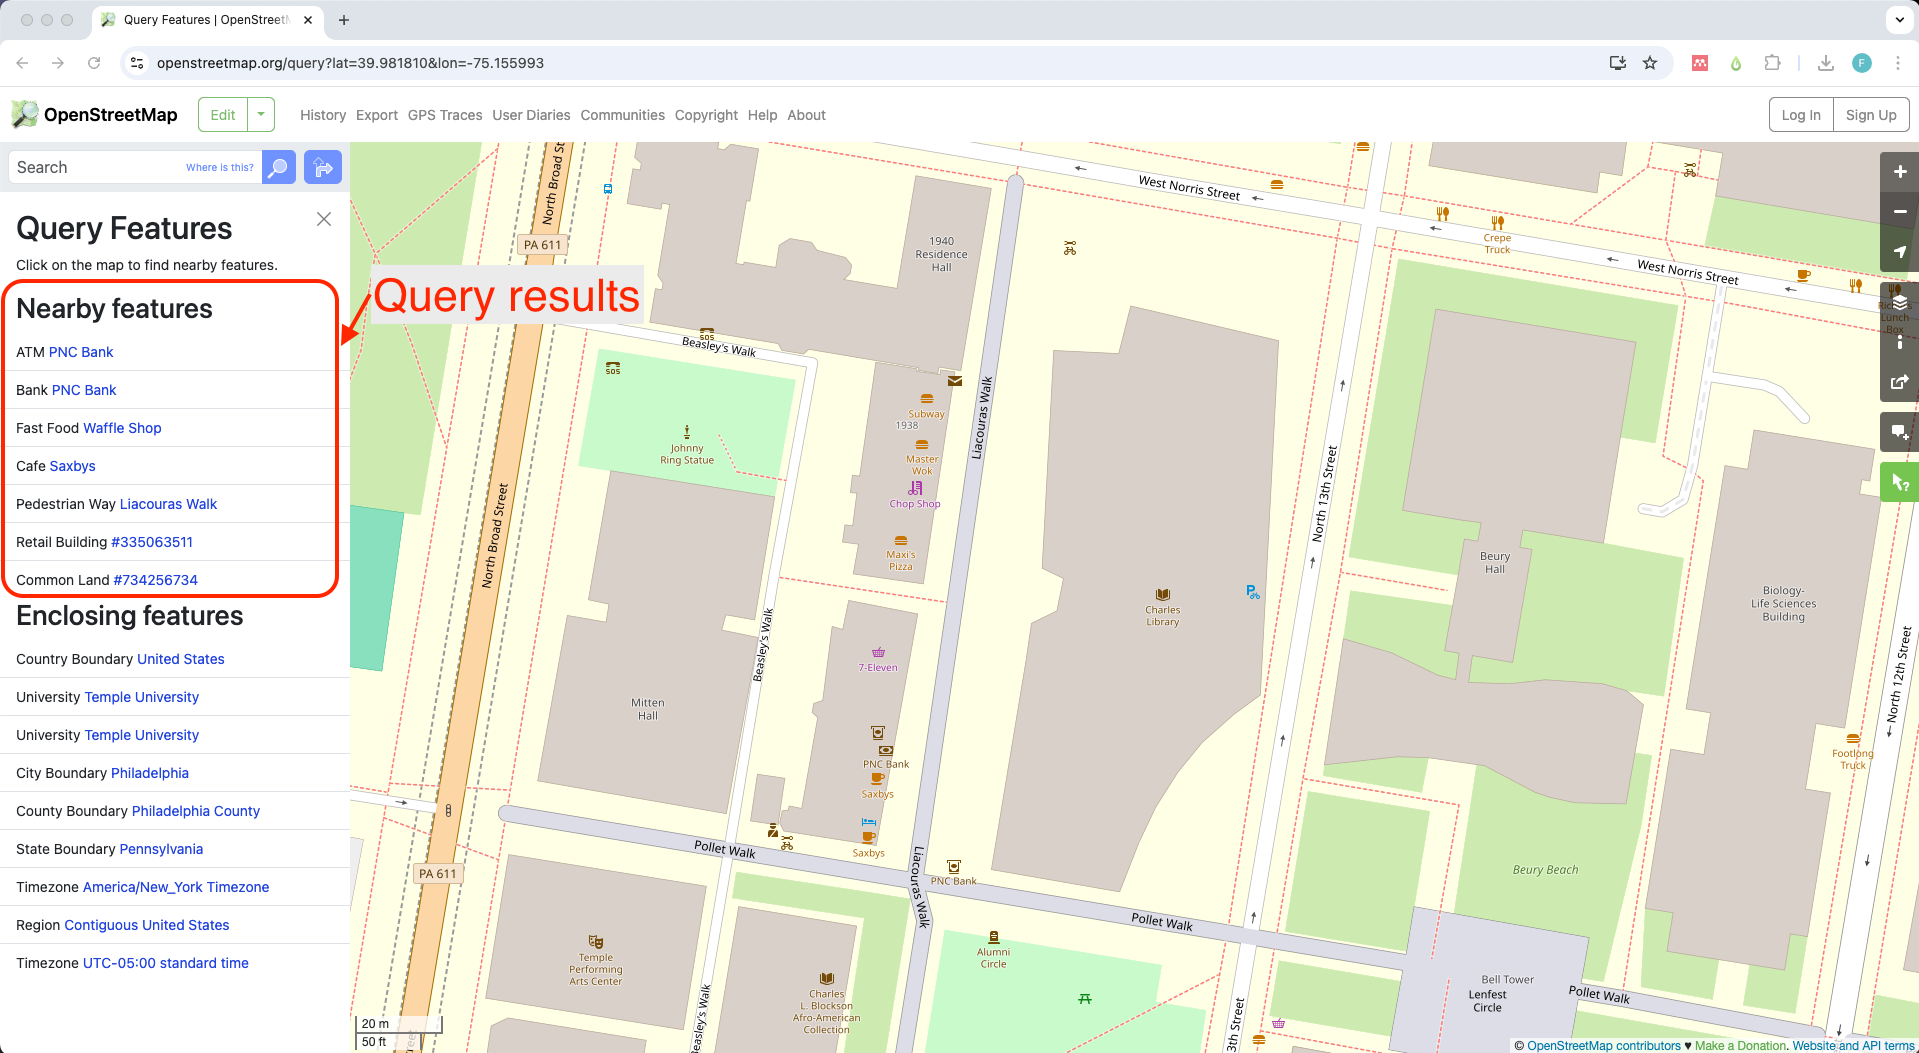
\includegraphics[keepaspectratio]{./images/queryosm1.png}}

{07} \emph{Explore the results.}

If you click on any of the results, the left side panel will show the
element details and tags. In this example, we clicked on `Saxbys', which
is a coffee shop by Charles Library.

As you can see, this element has five tags that describe it including
its name, opening hours, and wheelchair accessibility. An element can
have unlimited number of tags, however, some of them might be
auto-exclusive. See more details on OSM tagging system here.

\pandocbounded{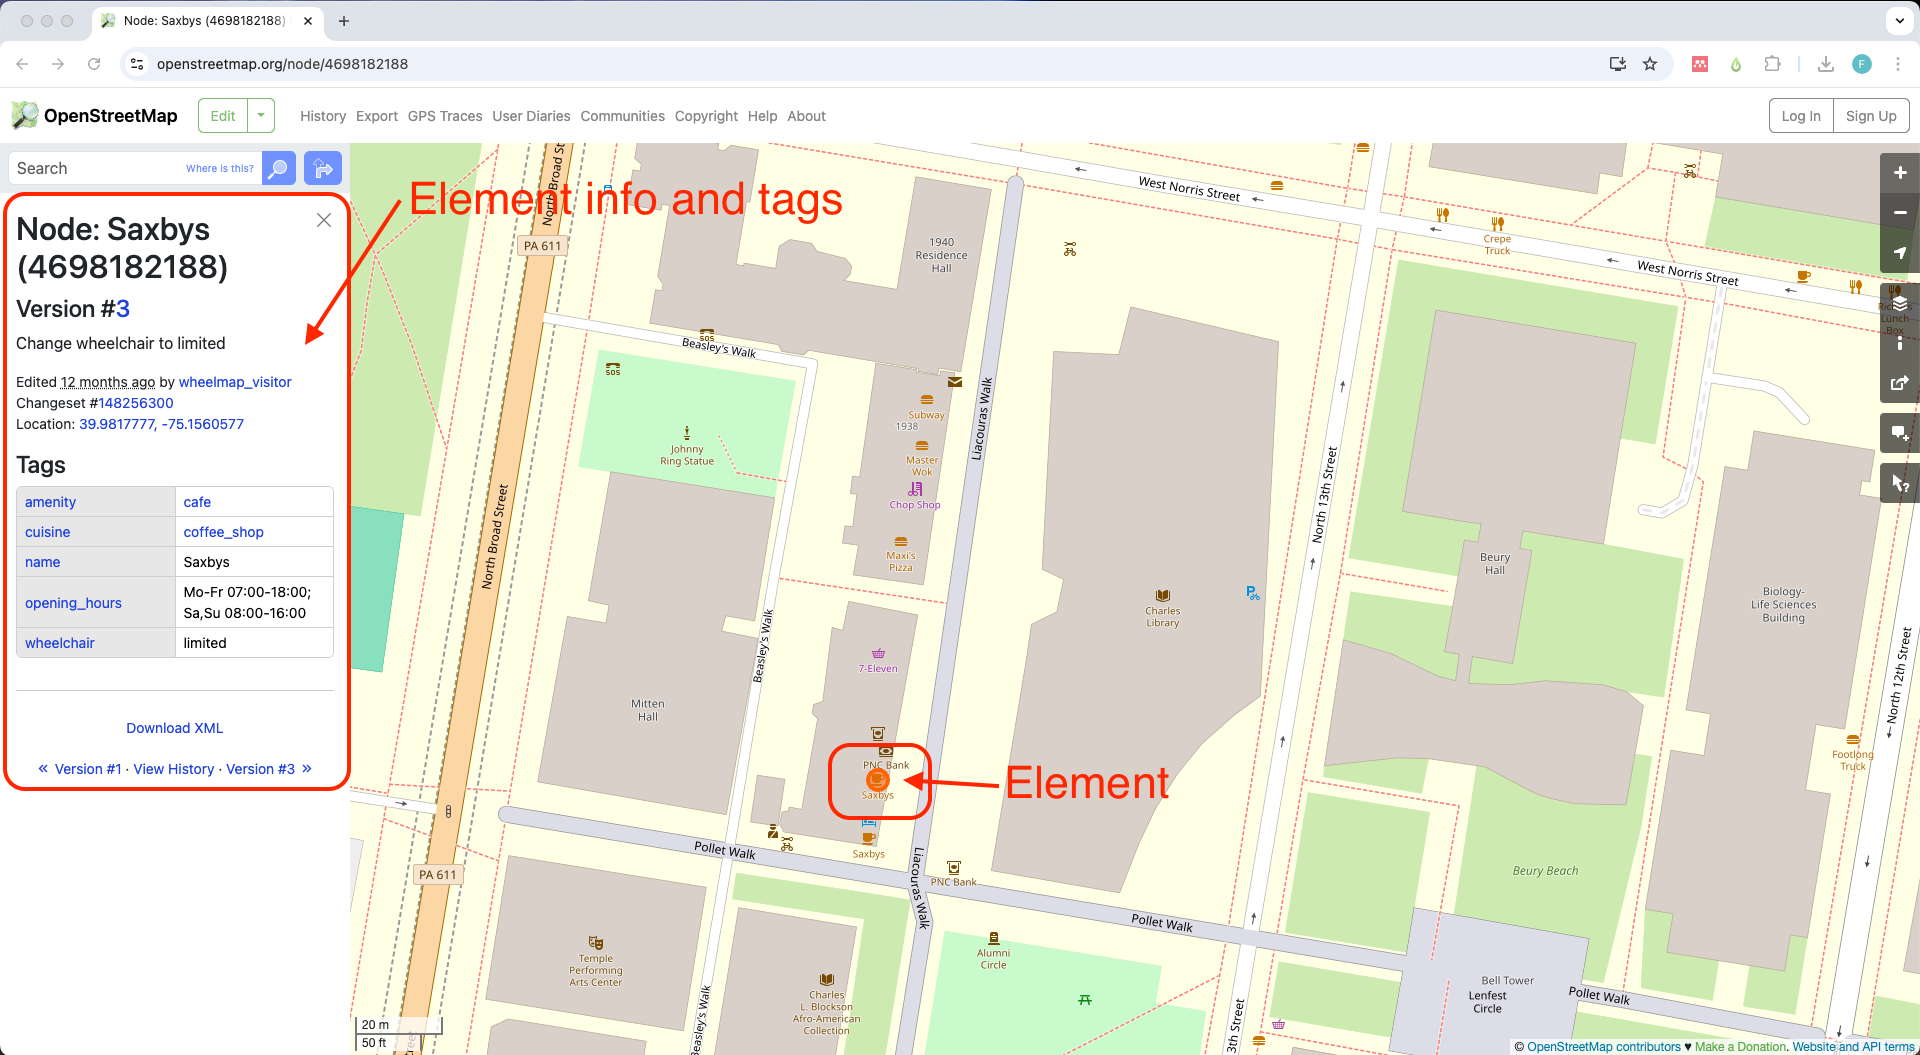
\includegraphics[keepaspectratio]{./images/queryosm2.png}}

\begin{tcolorbox}[enhanced jigsaw, opacitybacktitle=0.6, colframe=quarto-callout-warning-color-frame, arc=.35mm, leftrule=.75mm, toptitle=1mm, opacityback=0, titlerule=0mm, breakable, colback=white, colbacktitle=quarto-callout-warning-color!10!white, toprule=.15mm, bottomtitle=1mm, coltitle=black, title=\textcolor{quarto-callout-warning-color}{\faExclamationTriangle}\hspace{0.5em}{Warning!}, left=2mm, rightrule=.15mm, bottomrule=.15mm]

To add or modify tags and elements on the map you need to sign up for an
OSM account \href{https://www.openstreetmap.org/user/new}{here.}

\end{tcolorbox}

\subsection{In Overture Maps}\label{in-overture-maps}

{01} \emph{Go to
\href{https://explore.overturemaps.org/\#15/38.90678/-77.03649}{https://explore.overturemaps.org/}
on your web browser}

\pandocbounded{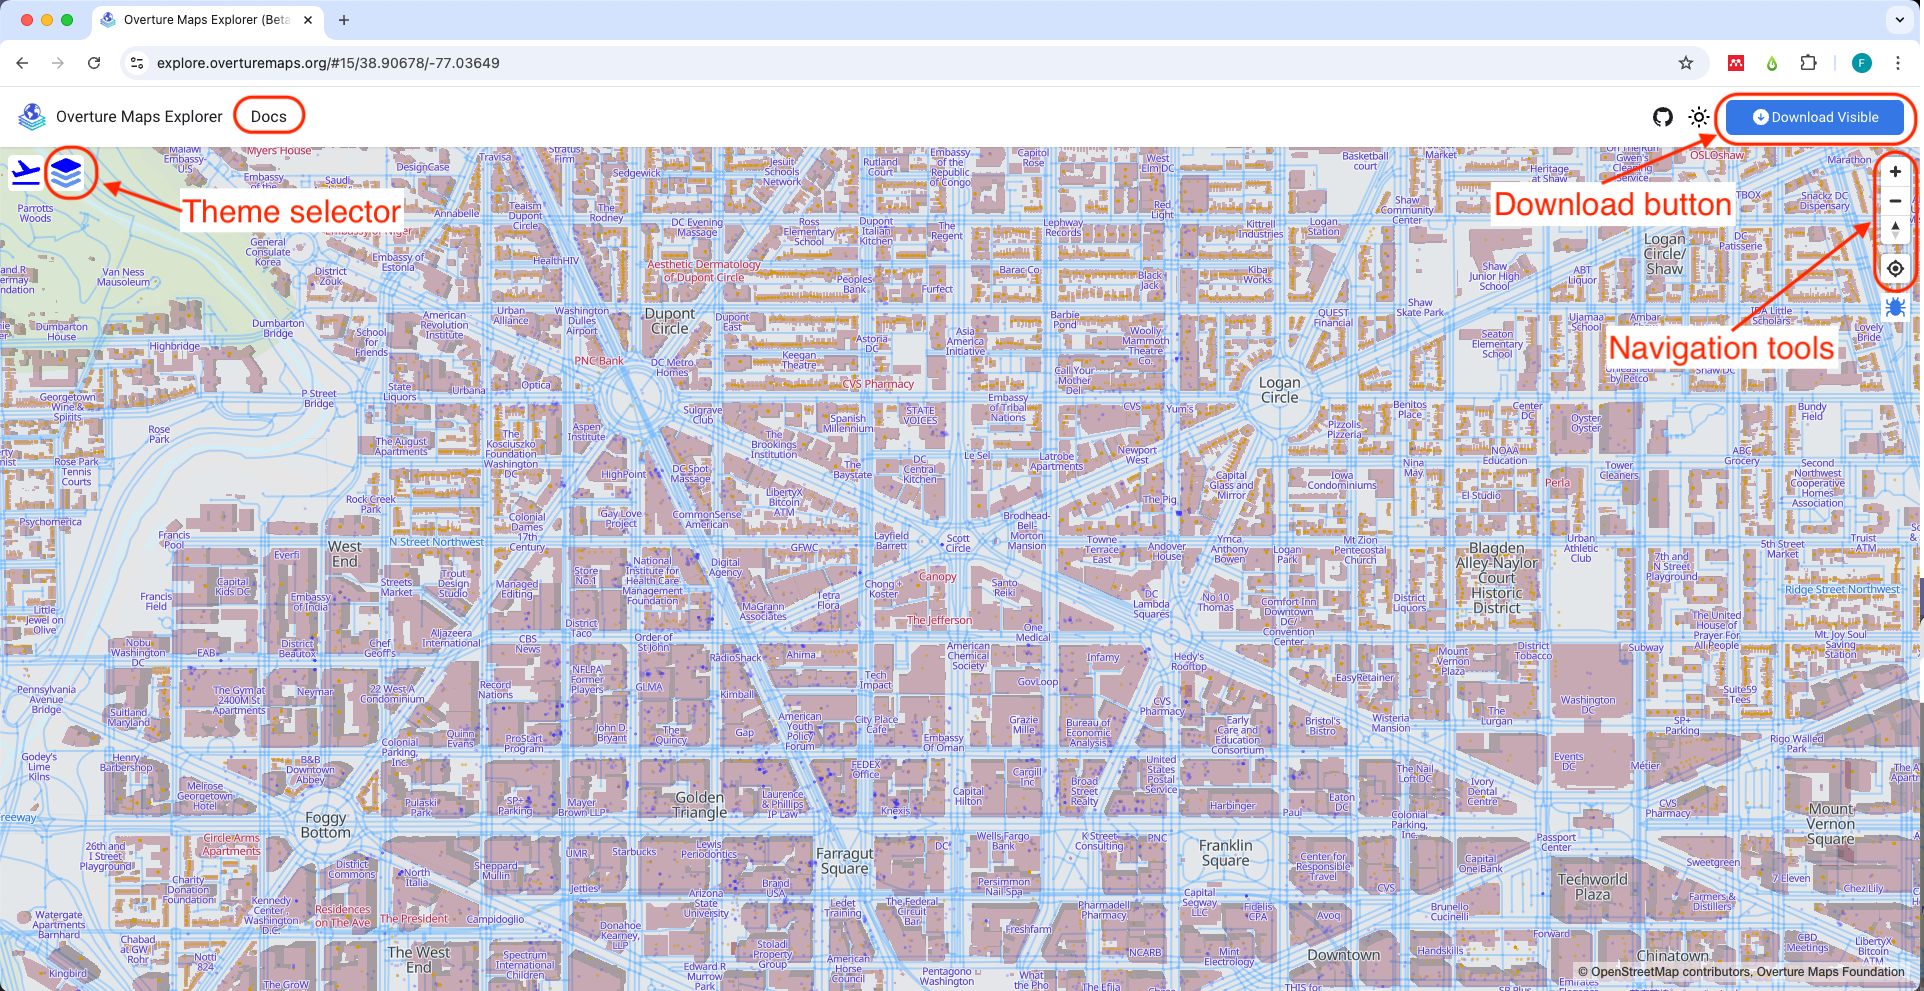
\includegraphics[keepaspectratio]{./images/overture_tools.png}}

{02} \emph{Find your location on the map}

Unlike OSM, the Overture Maps explorer does not have a search bar. The
best way to find a location is either clicking on the `Find my location'
button
\pandocbounded{
\includegraphics[keepaspectratio]{./images/overture_loc.png}}
or using the navigation controls (zoom in and zoom out).

\begin{tcolorbox}[enhanced jigsaw, opacitybacktitle=0.6, colframe=quarto-callout-caution-color-frame, arc=.35mm, leftrule=.75mm, toptitle=1mm, opacityback=0, titlerule=0mm, breakable, colback=white, colbacktitle=quarto-callout-caution-color!10!white, toprule=.15mm, bottomtitle=1mm, coltitle=black, title=\textcolor{quarto-callout-caution-color}{\faFire}\hspace{0.5em}{Allow access to your location}, left=2mm, rightrule=.15mm, bottomrule=.15mm]

The first time you use the `Find my location' tool, you will be asked to
allow the browser access. If you are ok with this, simply click on
`Allow this time'.

\begin{center}
\pandocbounded{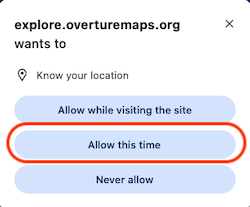
\includegraphics[keepaspectratio]{./images/overture_allow.png}}
\end{center}

\end{tcolorbox}

\pandocbounded{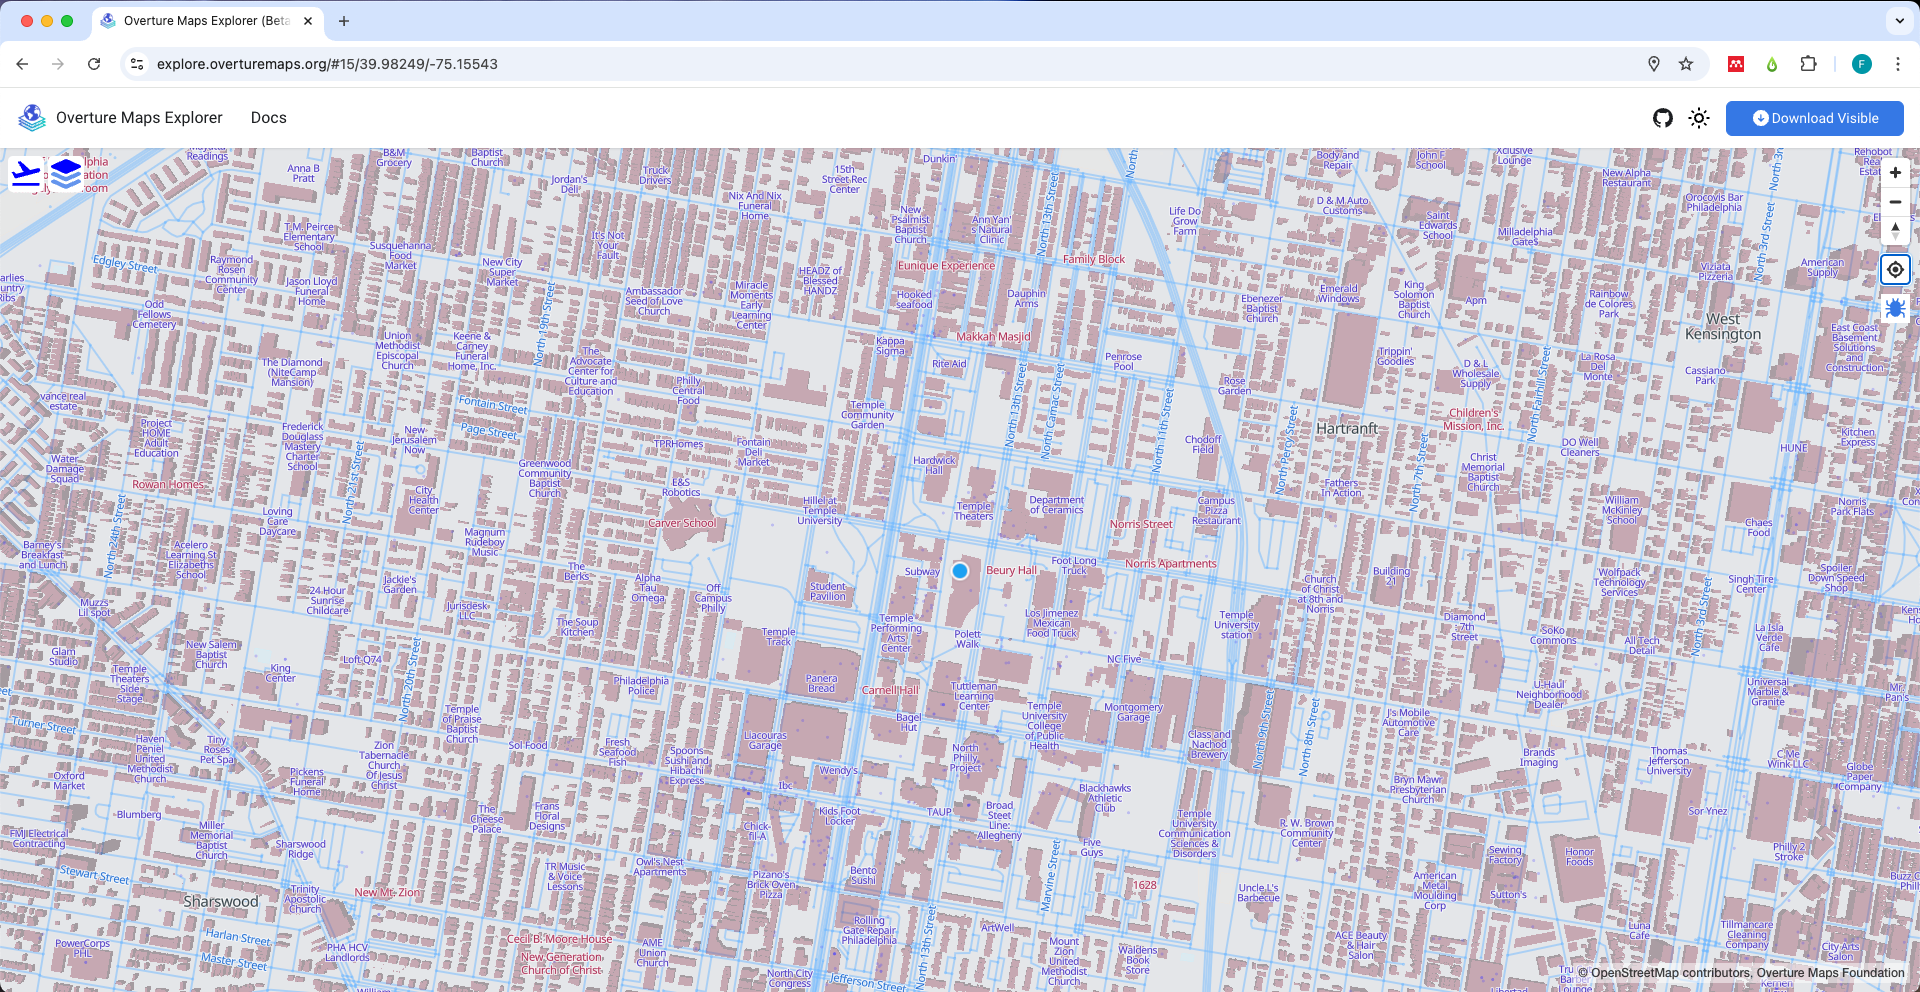
\includegraphics[keepaspectratio]{./images/overture_charles.png}}

{03} \emph{Click on any of the features you see on the map}

When you click on any feature on the map, a popup window will display
the feature(s) you clicked on, the bounding features (those that contain
the clicked feature, like the city, the county it is on). This popup
window will display the names of the features along with icons that
represent the feature `type'. In this example we can see there is a
`Charles Library' place
\pandocbounded{
\includegraphics[keepaspectratio]{./images/overture_place.png}}
and building
\pandocbounded{
\includegraphics[keepaspectratio]{./images/overture_building.png}}.

\pandocbounded{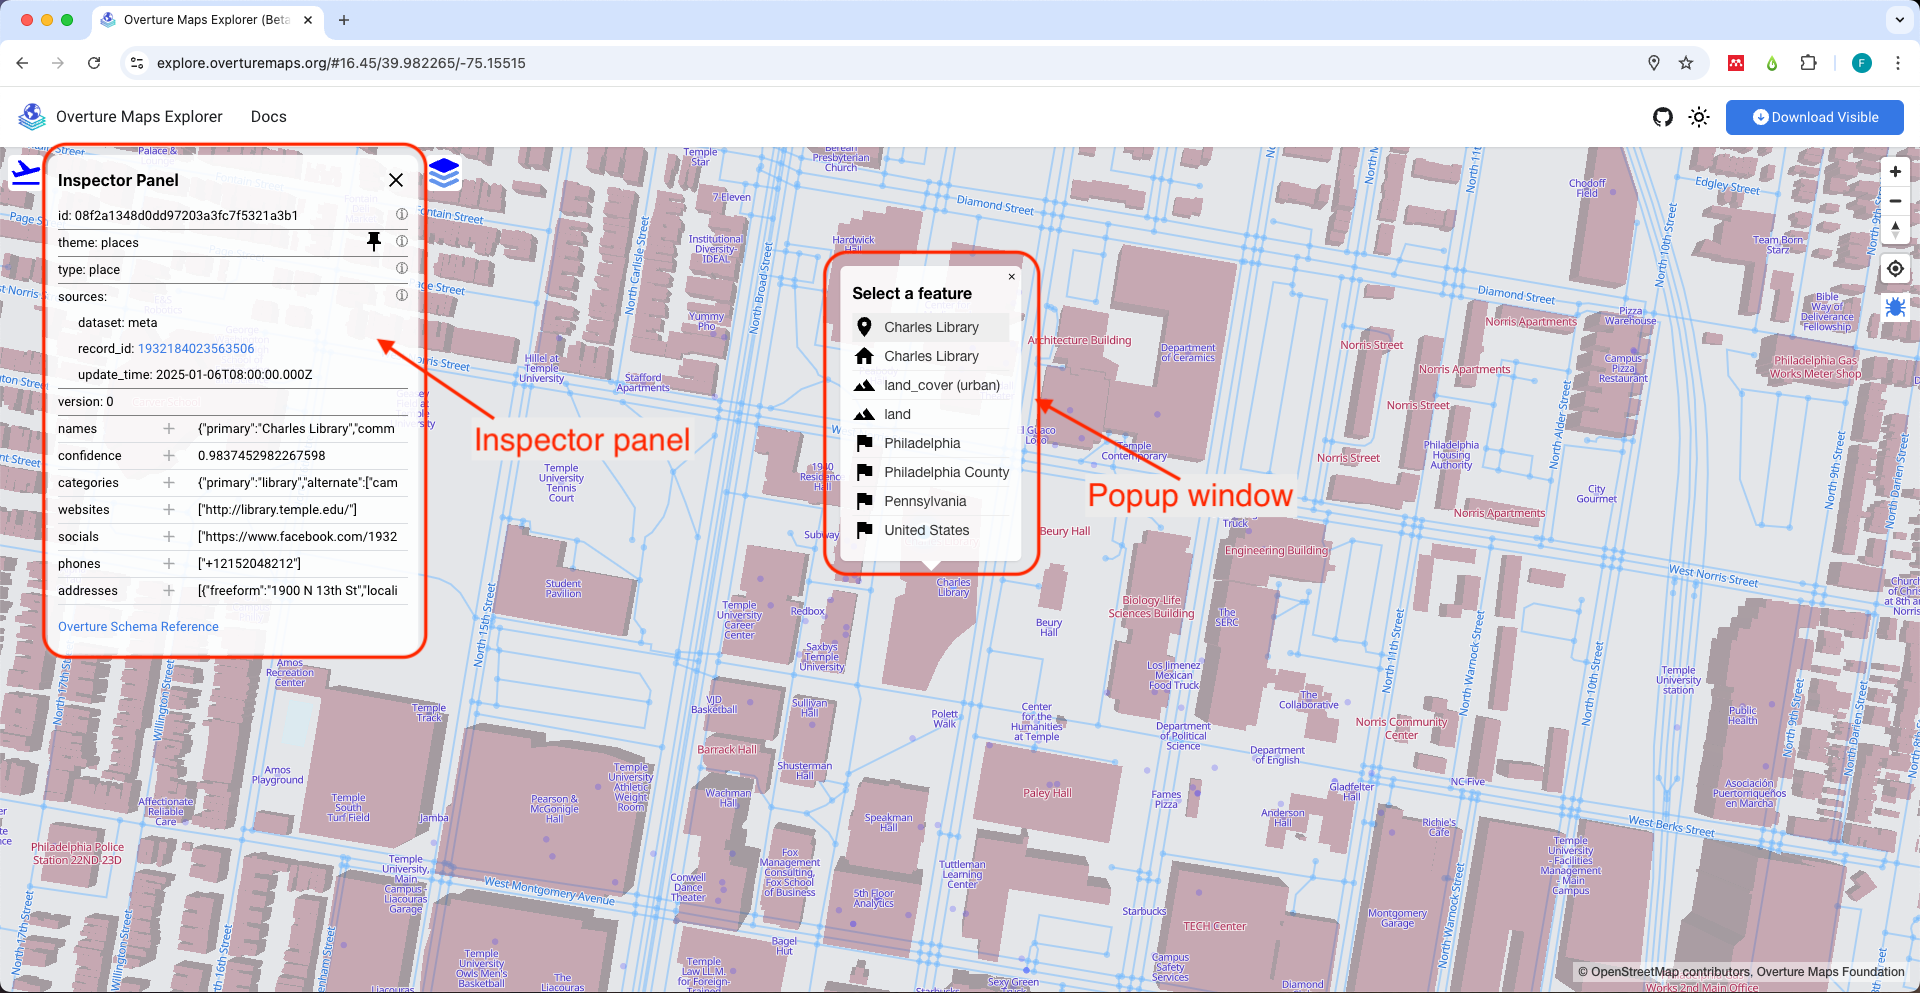
\includegraphics[keepaspectratio]{./images/overture_panel.png}}

On the left side of the screen, an `Inspector Panel' will show the
properties of the selected feature, including: the type, sources, names
and others depending on the feature type.

\subsection{In QGIS}\label{in-qgis}

There are some ways to explore OpenStreetMap data in QGIS without
downloading the data. The easiest way to do this is using OSM raster
tiles. Follow the steps below to see OSM data in QGIS.

\begin{tcolorbox}[enhanced jigsaw, opacitybacktitle=0.6, colframe=quarto-callout-important-color-frame, arc=.35mm, leftrule=.75mm, toptitle=1mm, opacityback=0, titlerule=0mm, breakable, colback=white, colbacktitle=quarto-callout-important-color!10!white, toprule=.15mm, bottomtitle=1mm, coltitle=black, title=\textcolor{quarto-callout-important-color}{\faExclamation}\hspace{0.5em}{Install QGIS}, left=2mm, rightrule=.15mm, bottomrule=.15mm]

If you don't have QGIS installed, go to \url{https://qgis.org/download/}
and follow the instructions to download the latest version for you
operating system.

\end{tcolorbox}

{01} \emph{Open QGIS}

\pandocbounded{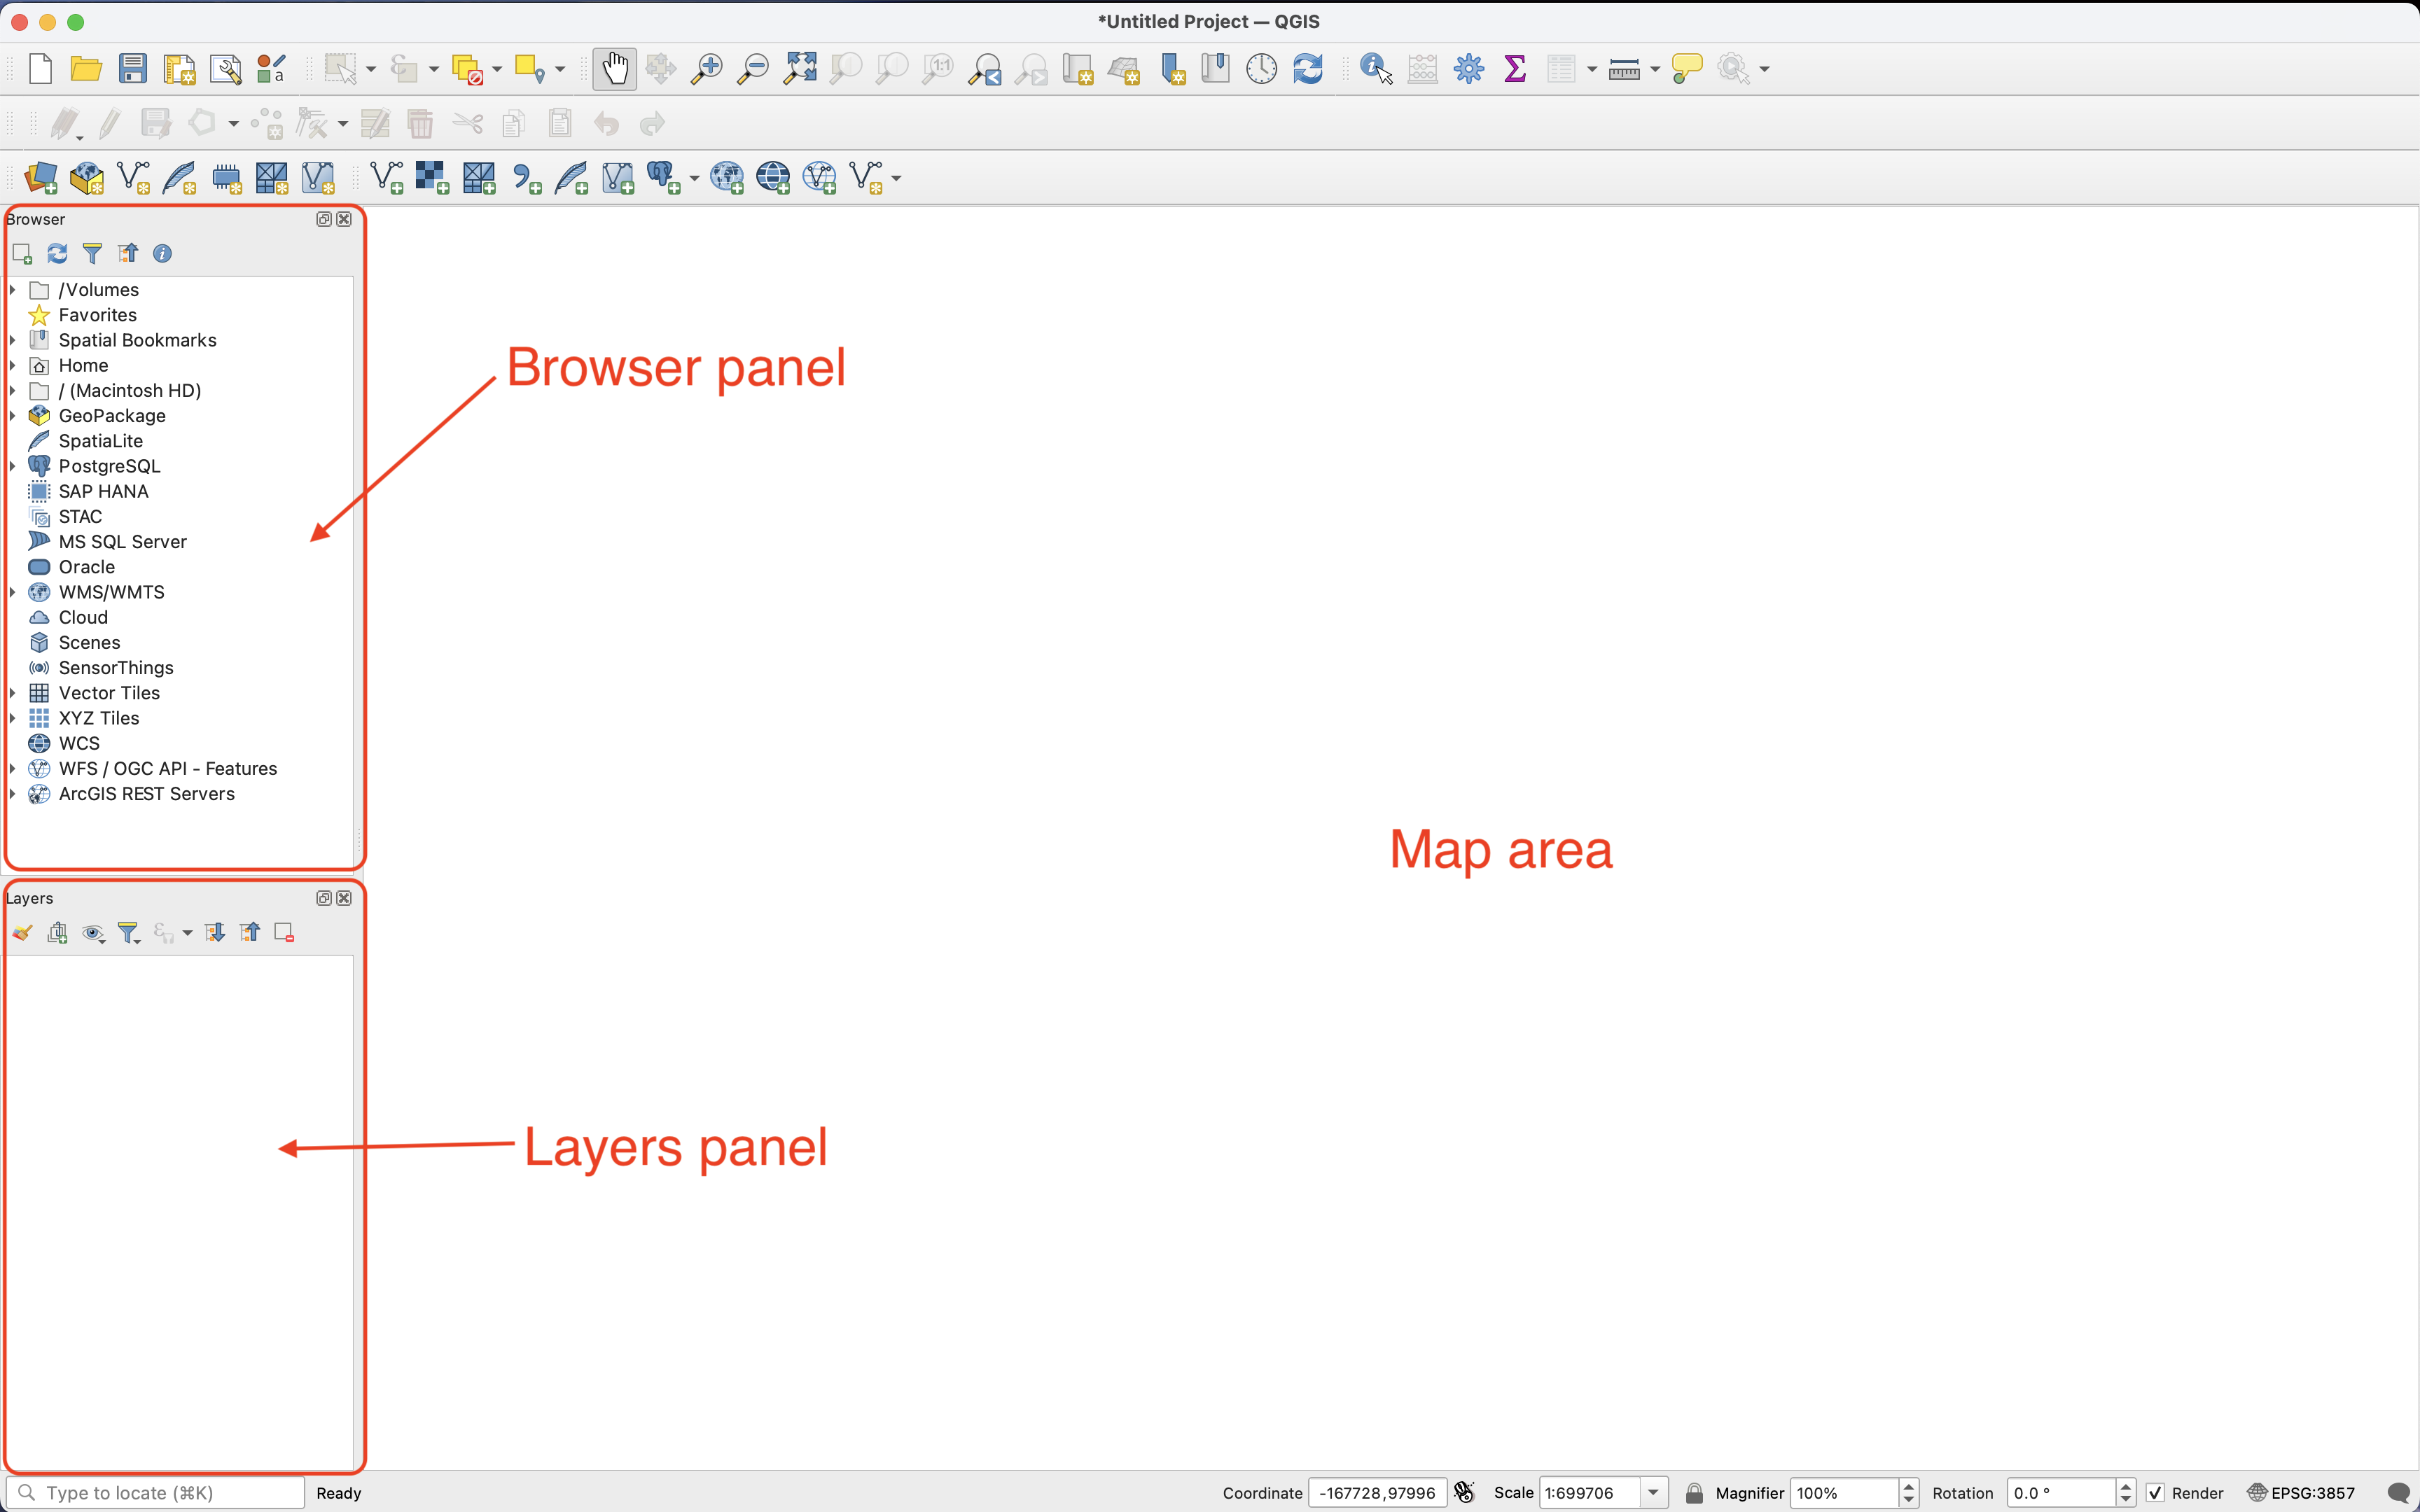
\includegraphics[keepaspectratio]{./images/qgis_main.png}}

{02} \emph{Add a raster tile connection}

In the Browser panel, right-click on \texttt{XYZ\ Tiles}, then click on
\texttt{New\ connection}.

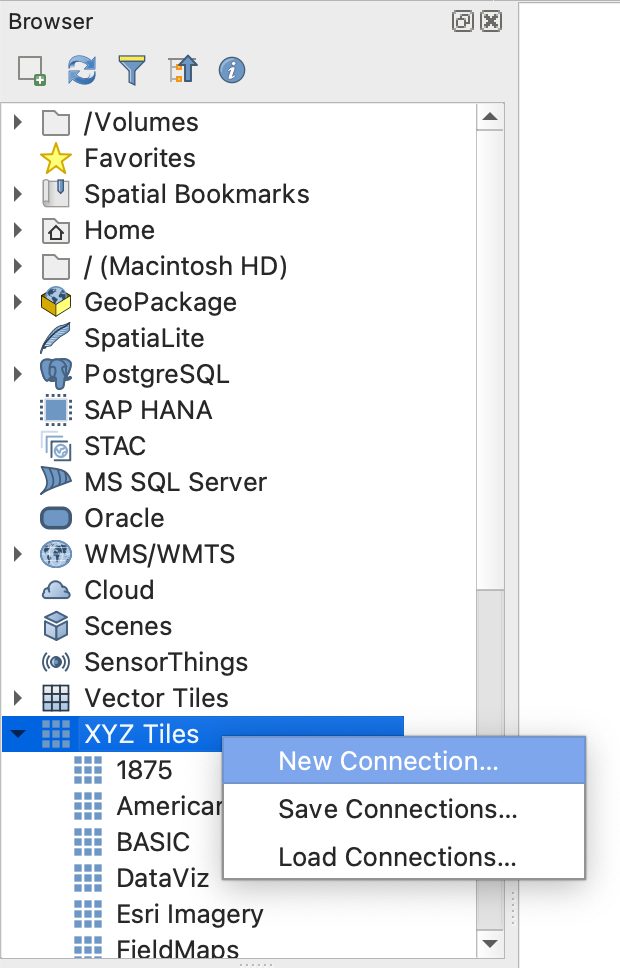
\includegraphics[width=0.3\linewidth,height=\textheight,keepaspectratio]{./images/qgis_new.png}

{03} \emph{Set the new XYZ connection}

In the new window, type \texttt{OSM} as the name for your connection.
Then copy and paste this line
\texttt{https://tile.openstreetmap.org/\{z\}/\{x\}/\{y\}.png} in the URL
space under `Connection Details'.

Then click \texttt{OK}.

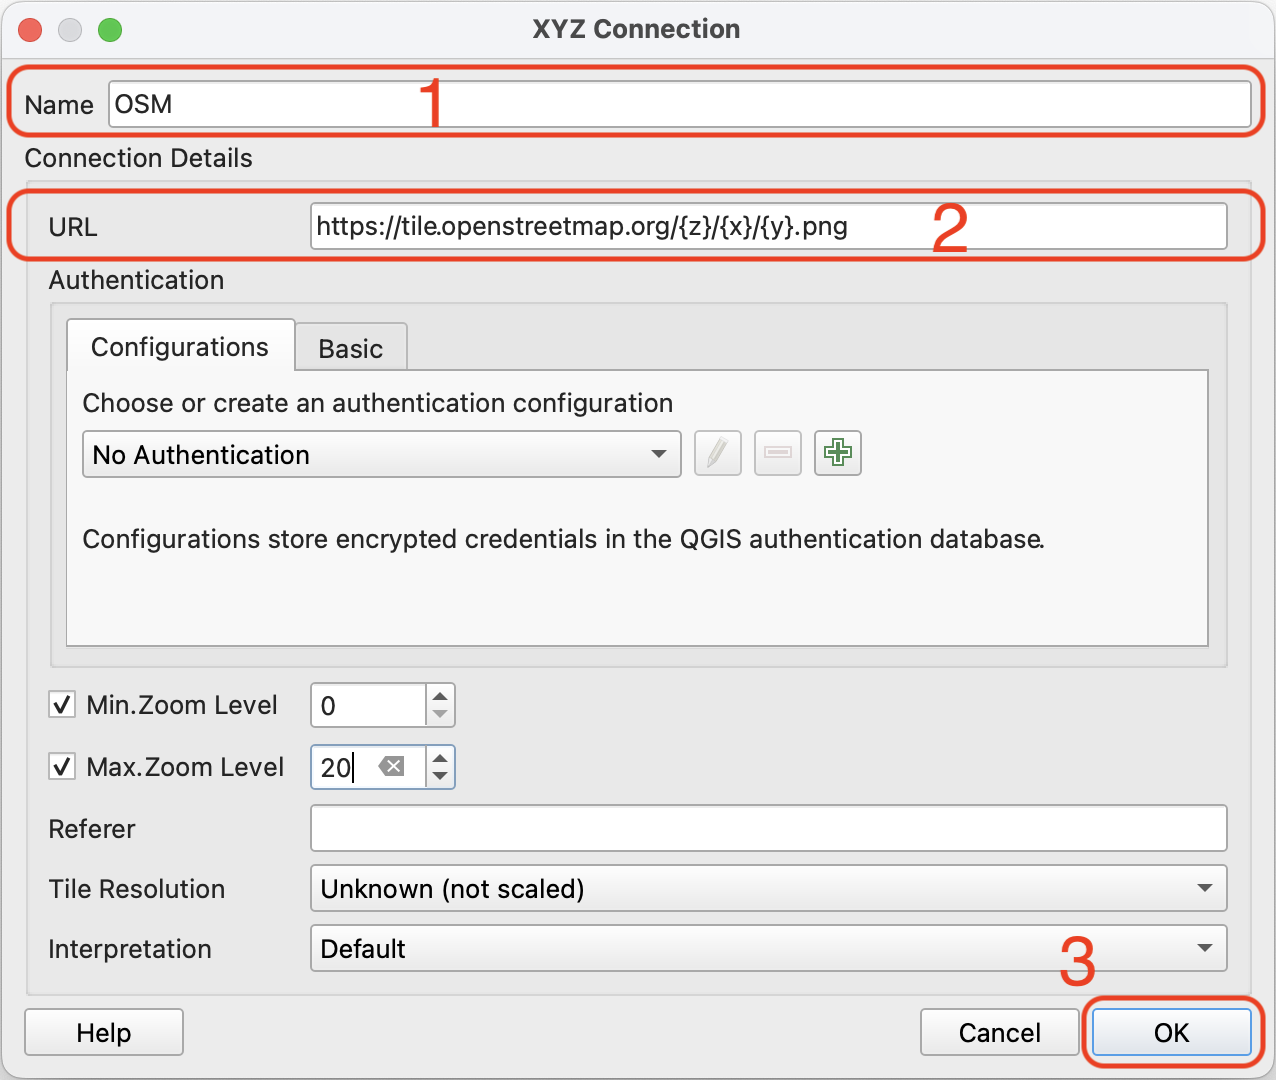
\includegraphics[width=0.5\linewidth,height=\textheight,keepaspectratio]{./images/qgis_new2.png}

{04} \emph{Add the XYZ tiles to the map}

Find the \texttt{OSM} XYZ raster tiles you created on previous step on
the Browser panel and drag it to the Layers panel or directly to the map
area.

\pandocbounded{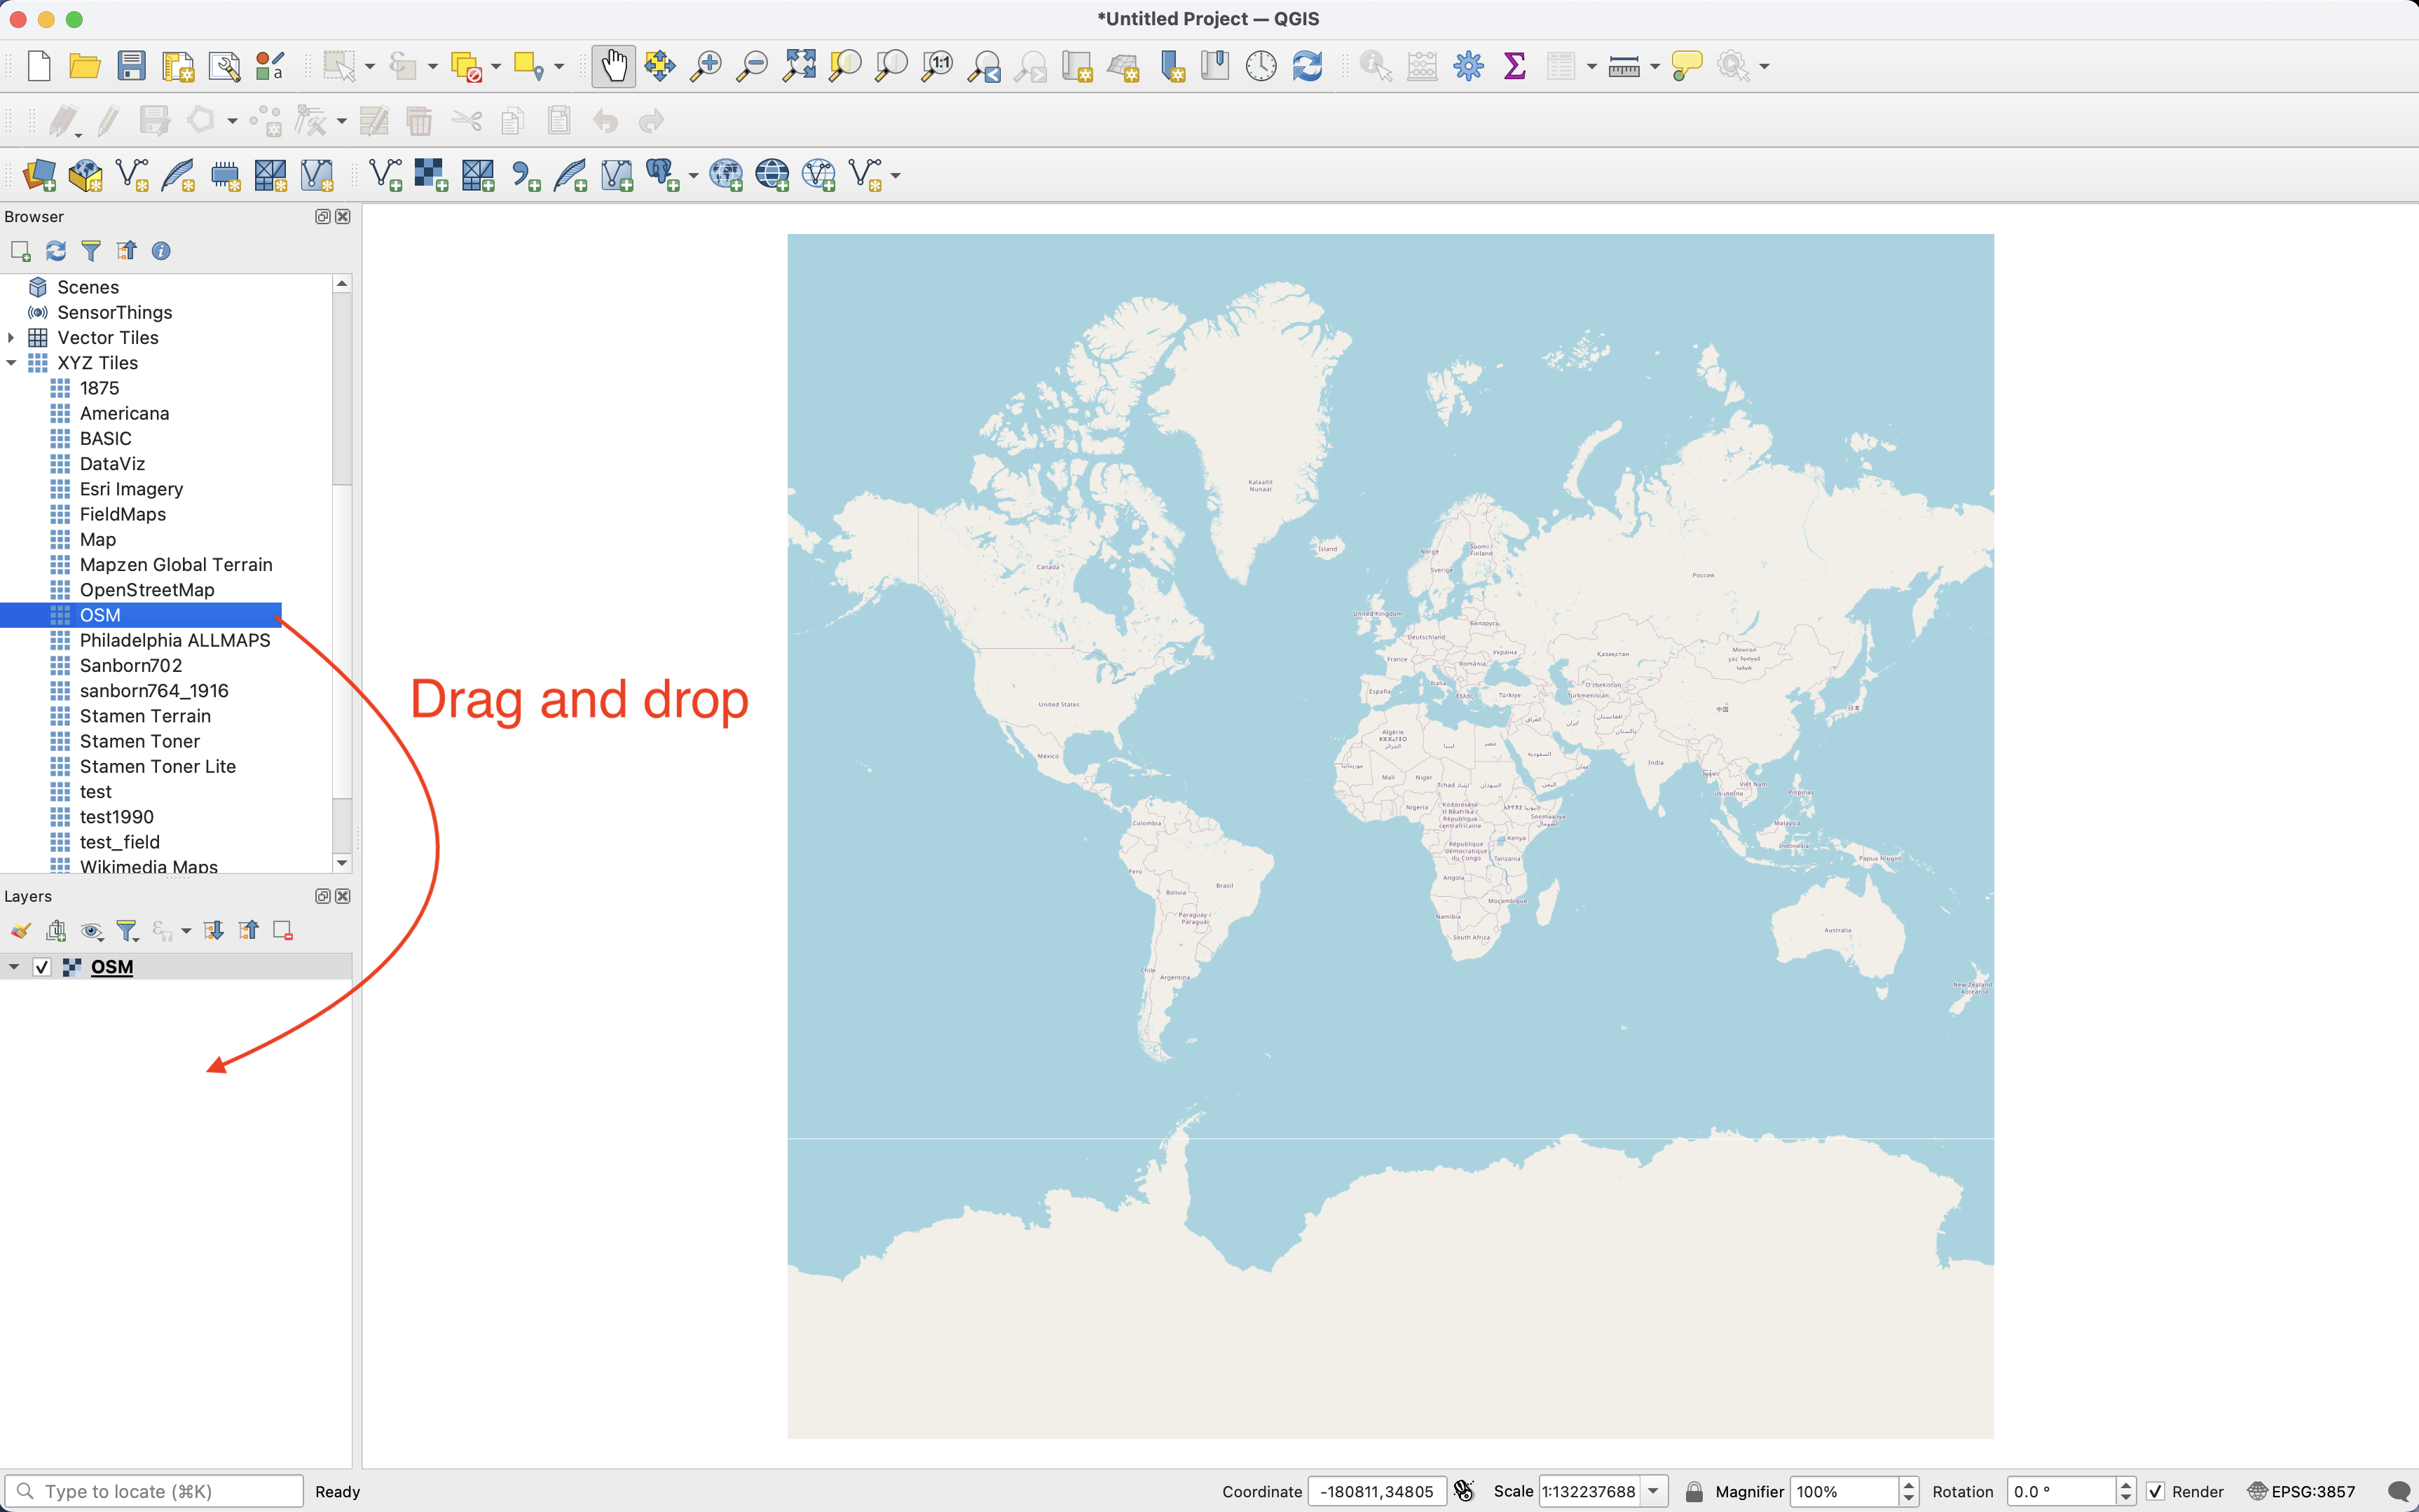
\includegraphics[keepaspectratio]{./images/qgis_osm.png}}

{05} \emph{Zoom in to the desired area on the map}

Using the zoom in tools located in the top of the screen on QGIS you can
locate the area you want to see. The map will show more details based on
the level of zoom you are in. Ypu can use this raster tiles as a basemap
in your projects.

\pandocbounded{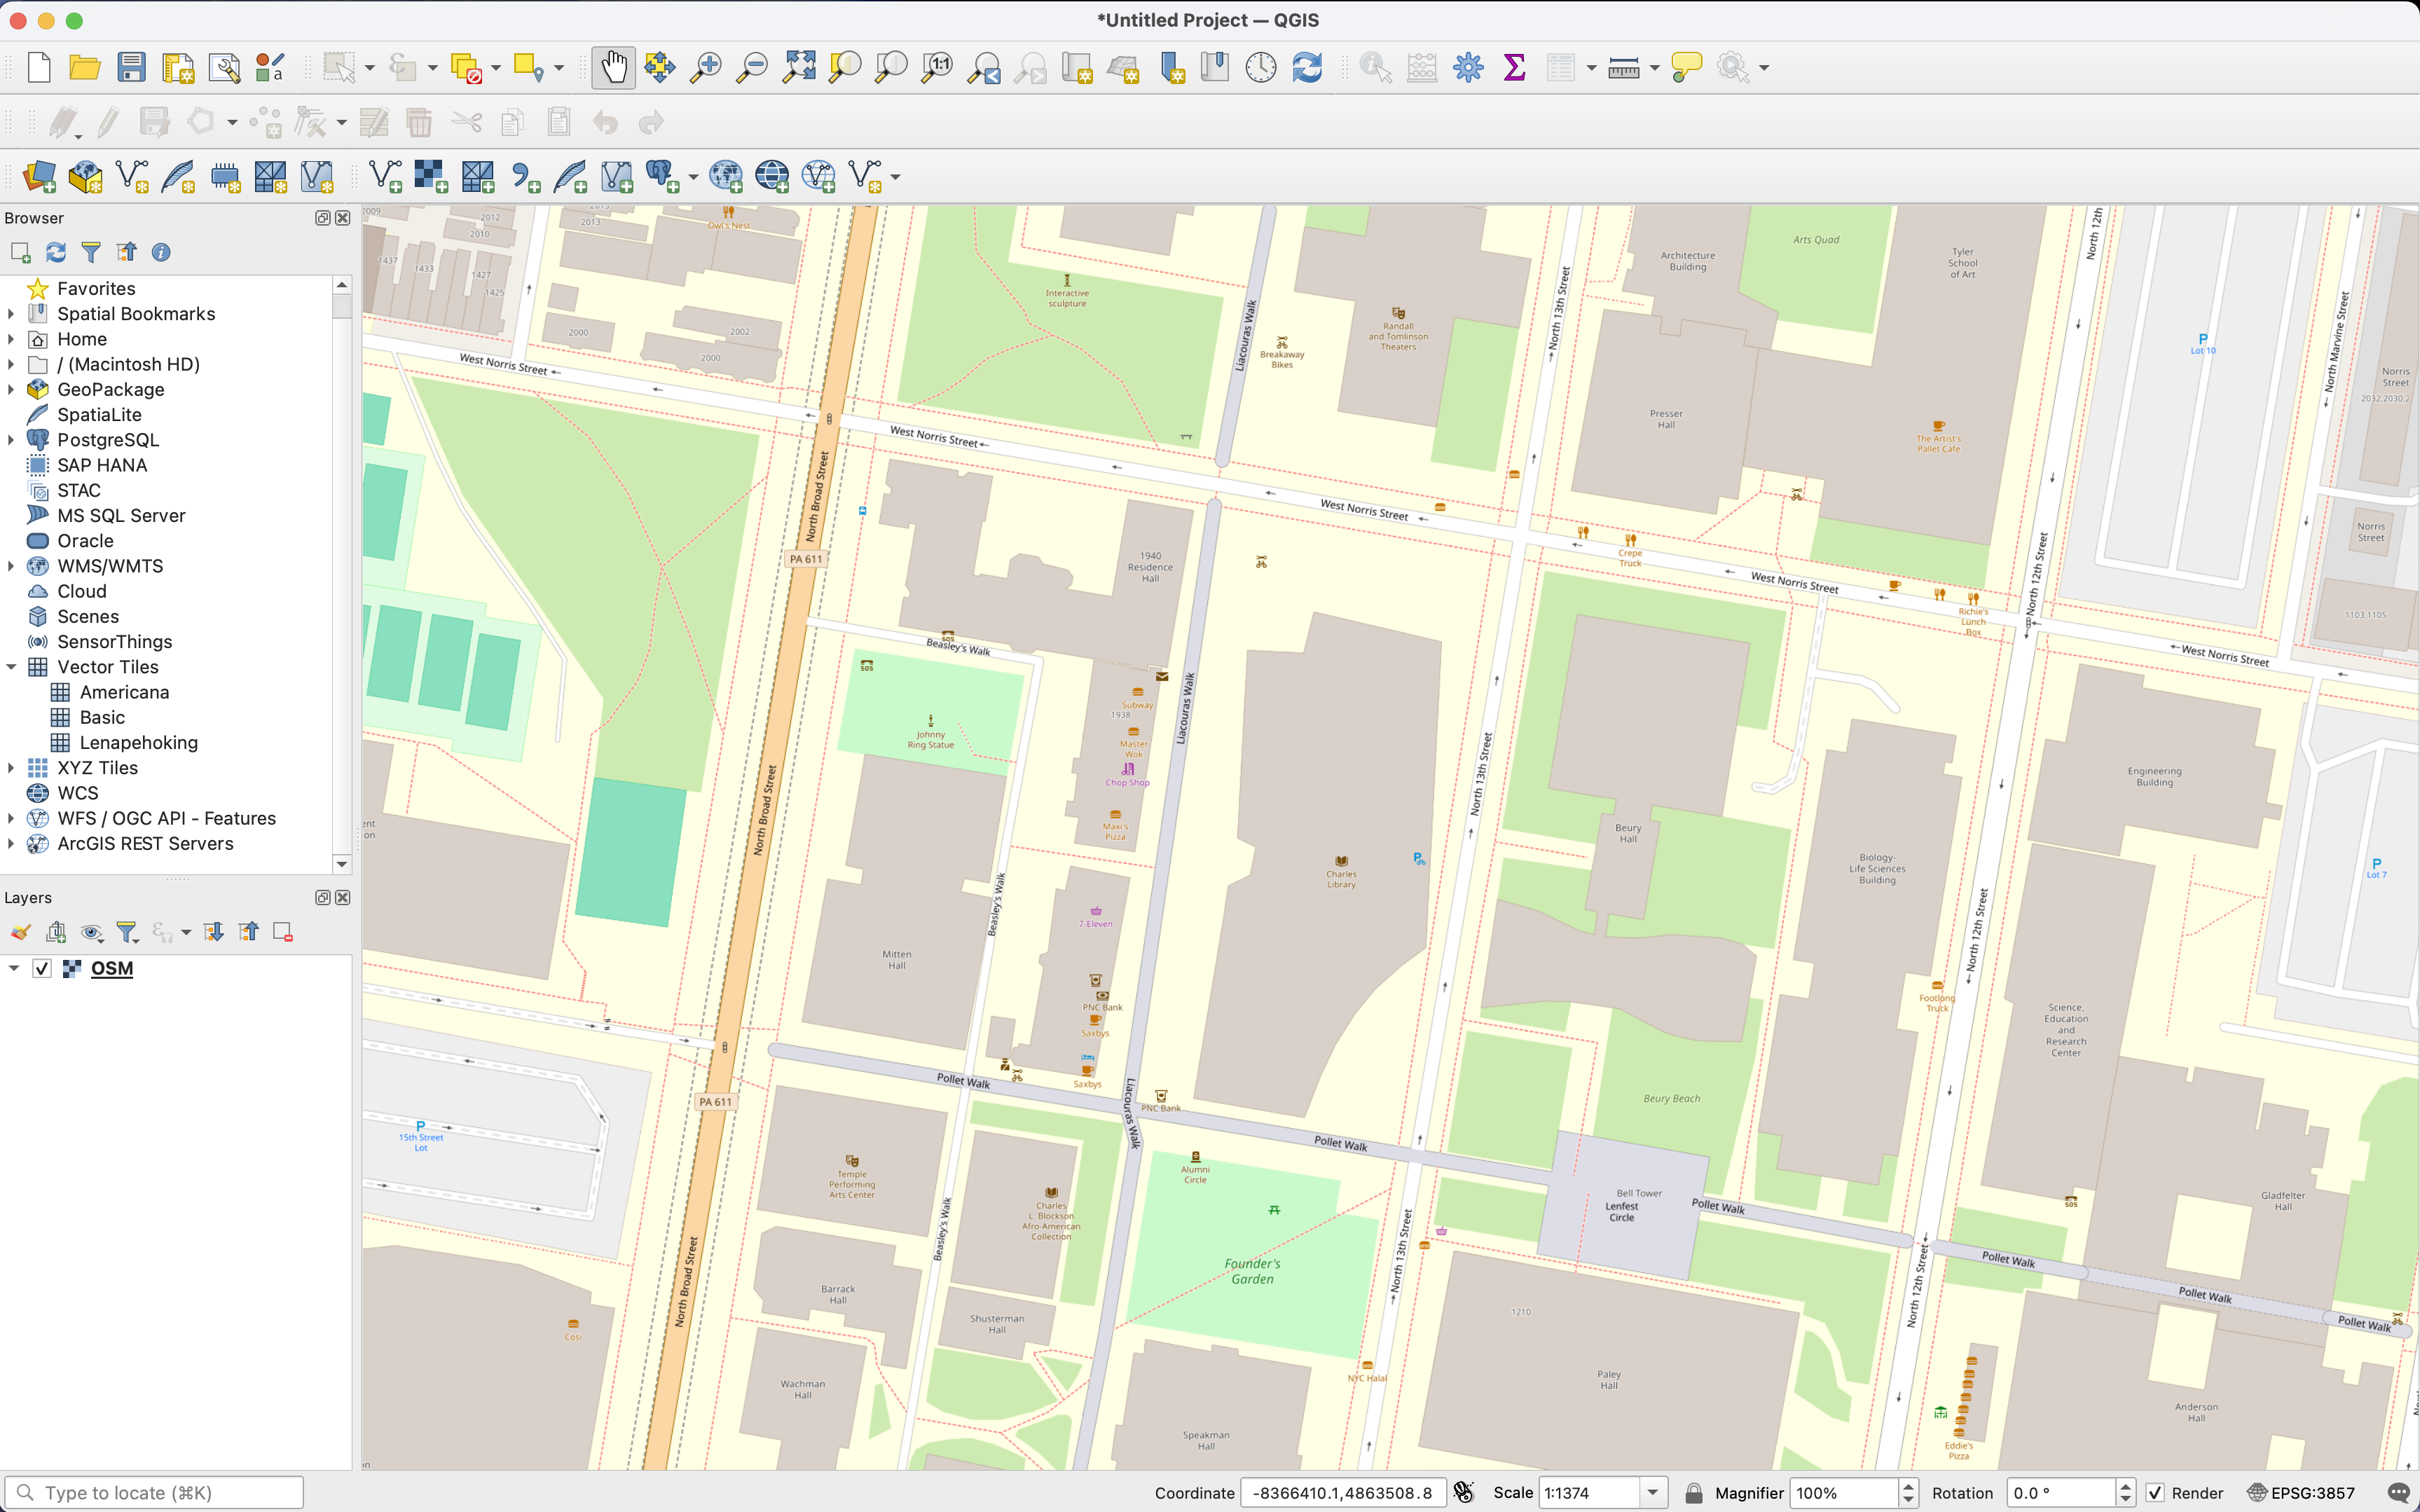
\includegraphics[keepaspectratio]{./images/qgis_map.png}}

\begin{tcolorbox}[enhanced jigsaw, opacitybacktitle=0.6, colframe=quarto-callout-warning-color-frame, arc=.35mm, leftrule=.75mm, toptitle=1mm, opacityback=0, titlerule=0mm, breakable, colback=white, colbacktitle=quarto-callout-warning-color!10!white, toprule=.15mm, bottomtitle=1mm, coltitle=black, title=\textcolor{quarto-callout-warning-color}{\faExclamationTriangle}\hspace{0.5em}{Warning!}, left=2mm, rightrule=.15mm, bottomrule=.15mm]

OSM tiles are served through the internet. The speed at which the map
loads depends on your internet connection.

\end{tcolorbox}

\section{Downloading the data}\label{downloading-the-data}

There are multiple ways to download data from OSM and Overture Maps. In
this tutorial we focus on how to download data directly to QGIS.

\subsection{From OSM to QGIS}\label{from-osm-to-qgis}

{01} \emph{Install QuickOSM plugin}

Open QGIS.

On the top menu bar click on `Plugins' and then on `Manage and Install
Plugins'.

\pandocbounded{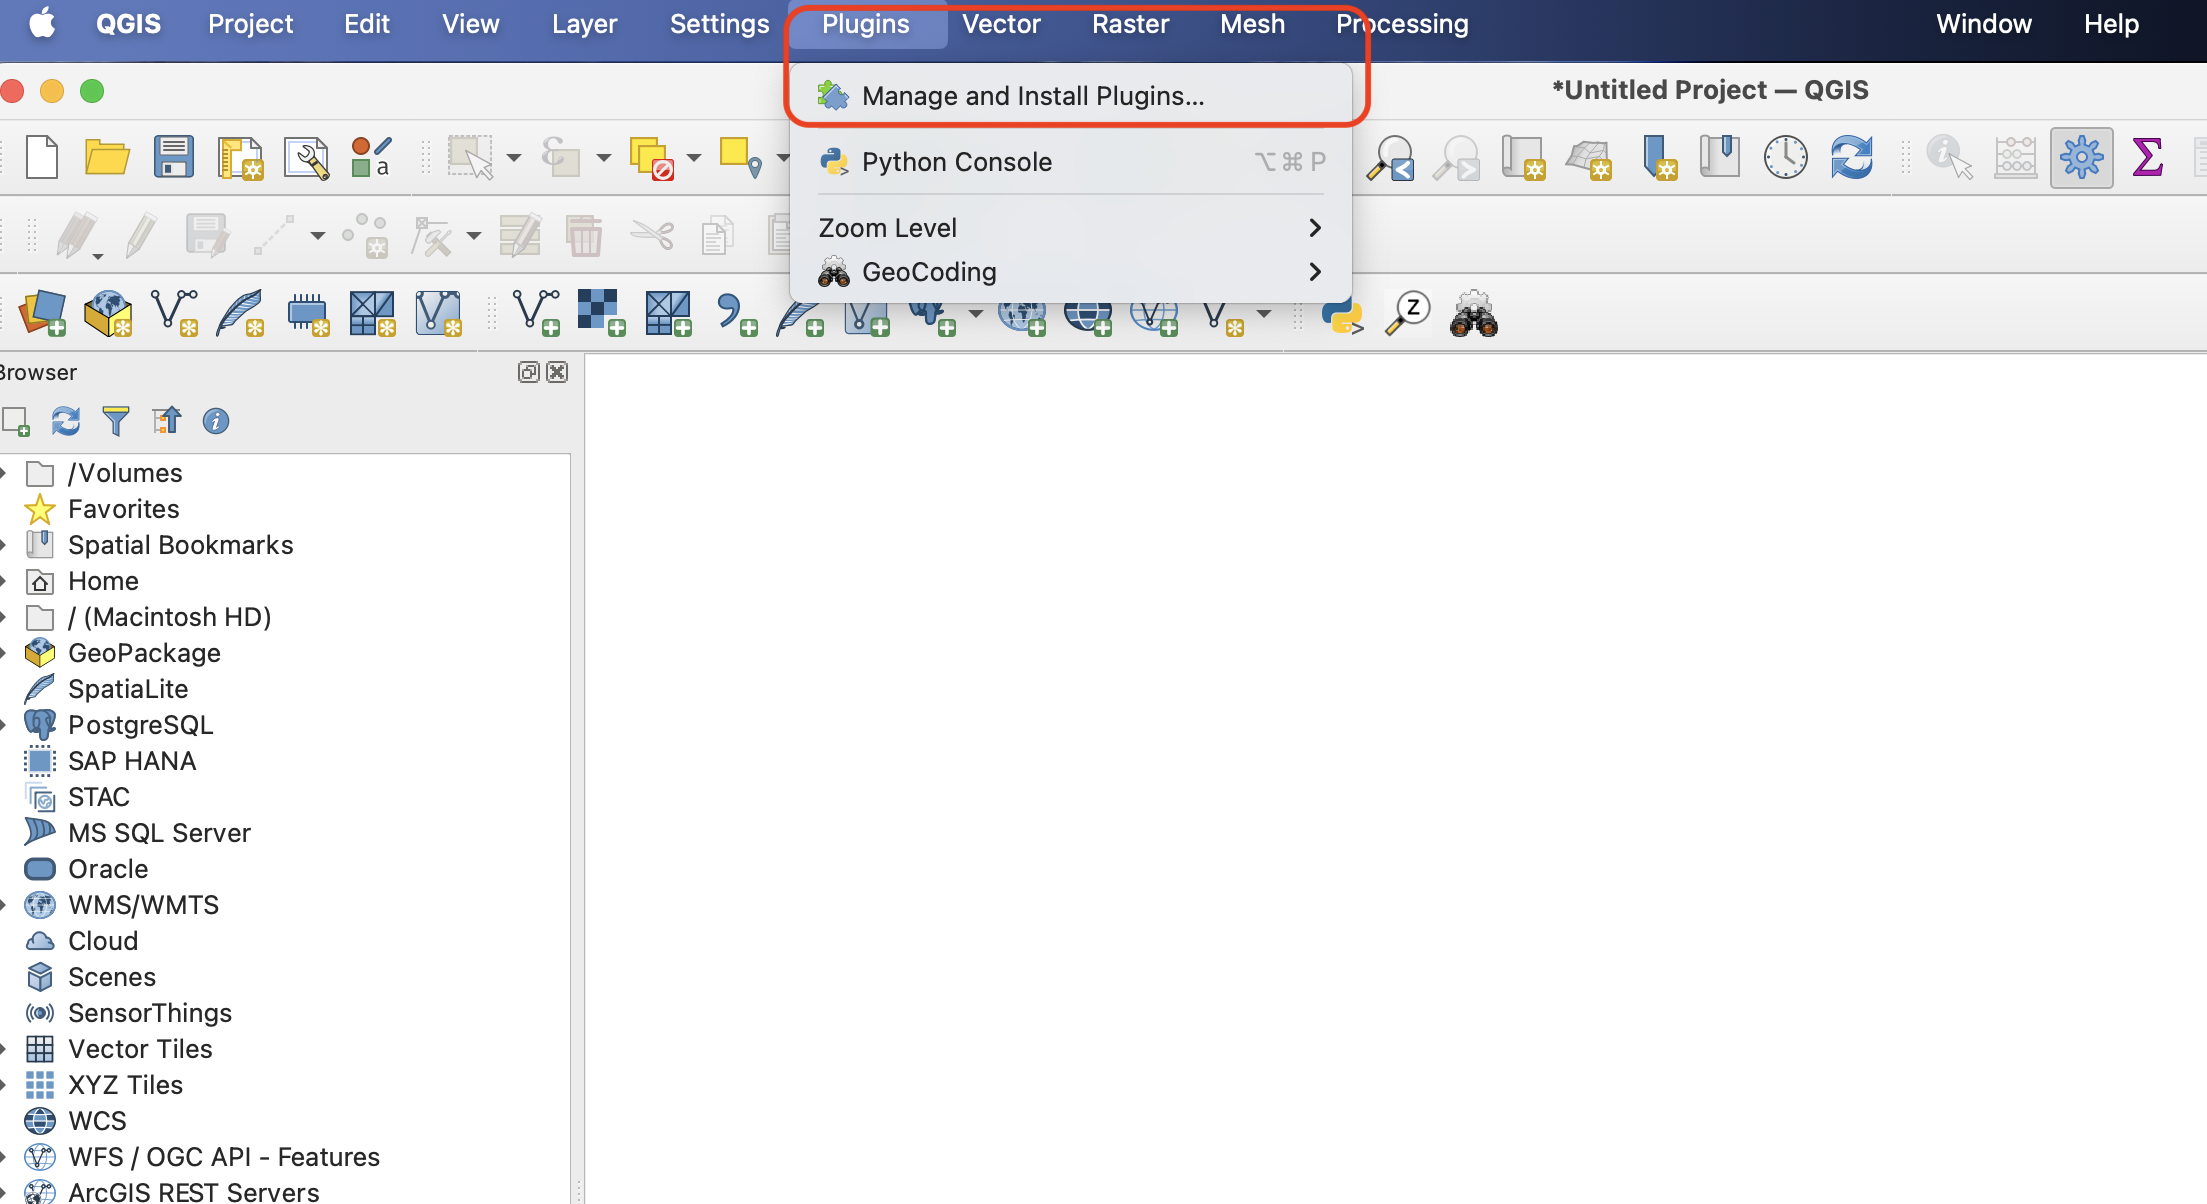
\includegraphics[keepaspectratio]{./images/qgis_mn.png}}

On the new window, in the search bar type \texttt{quickosm}, then click
on `Install plugin'. Once installed, close the plugins manager window.
Learn more about
\href{https://plugins.qgis.org/plugins/QuickOSM/}{QuickOSM plugin}

\pandocbounded{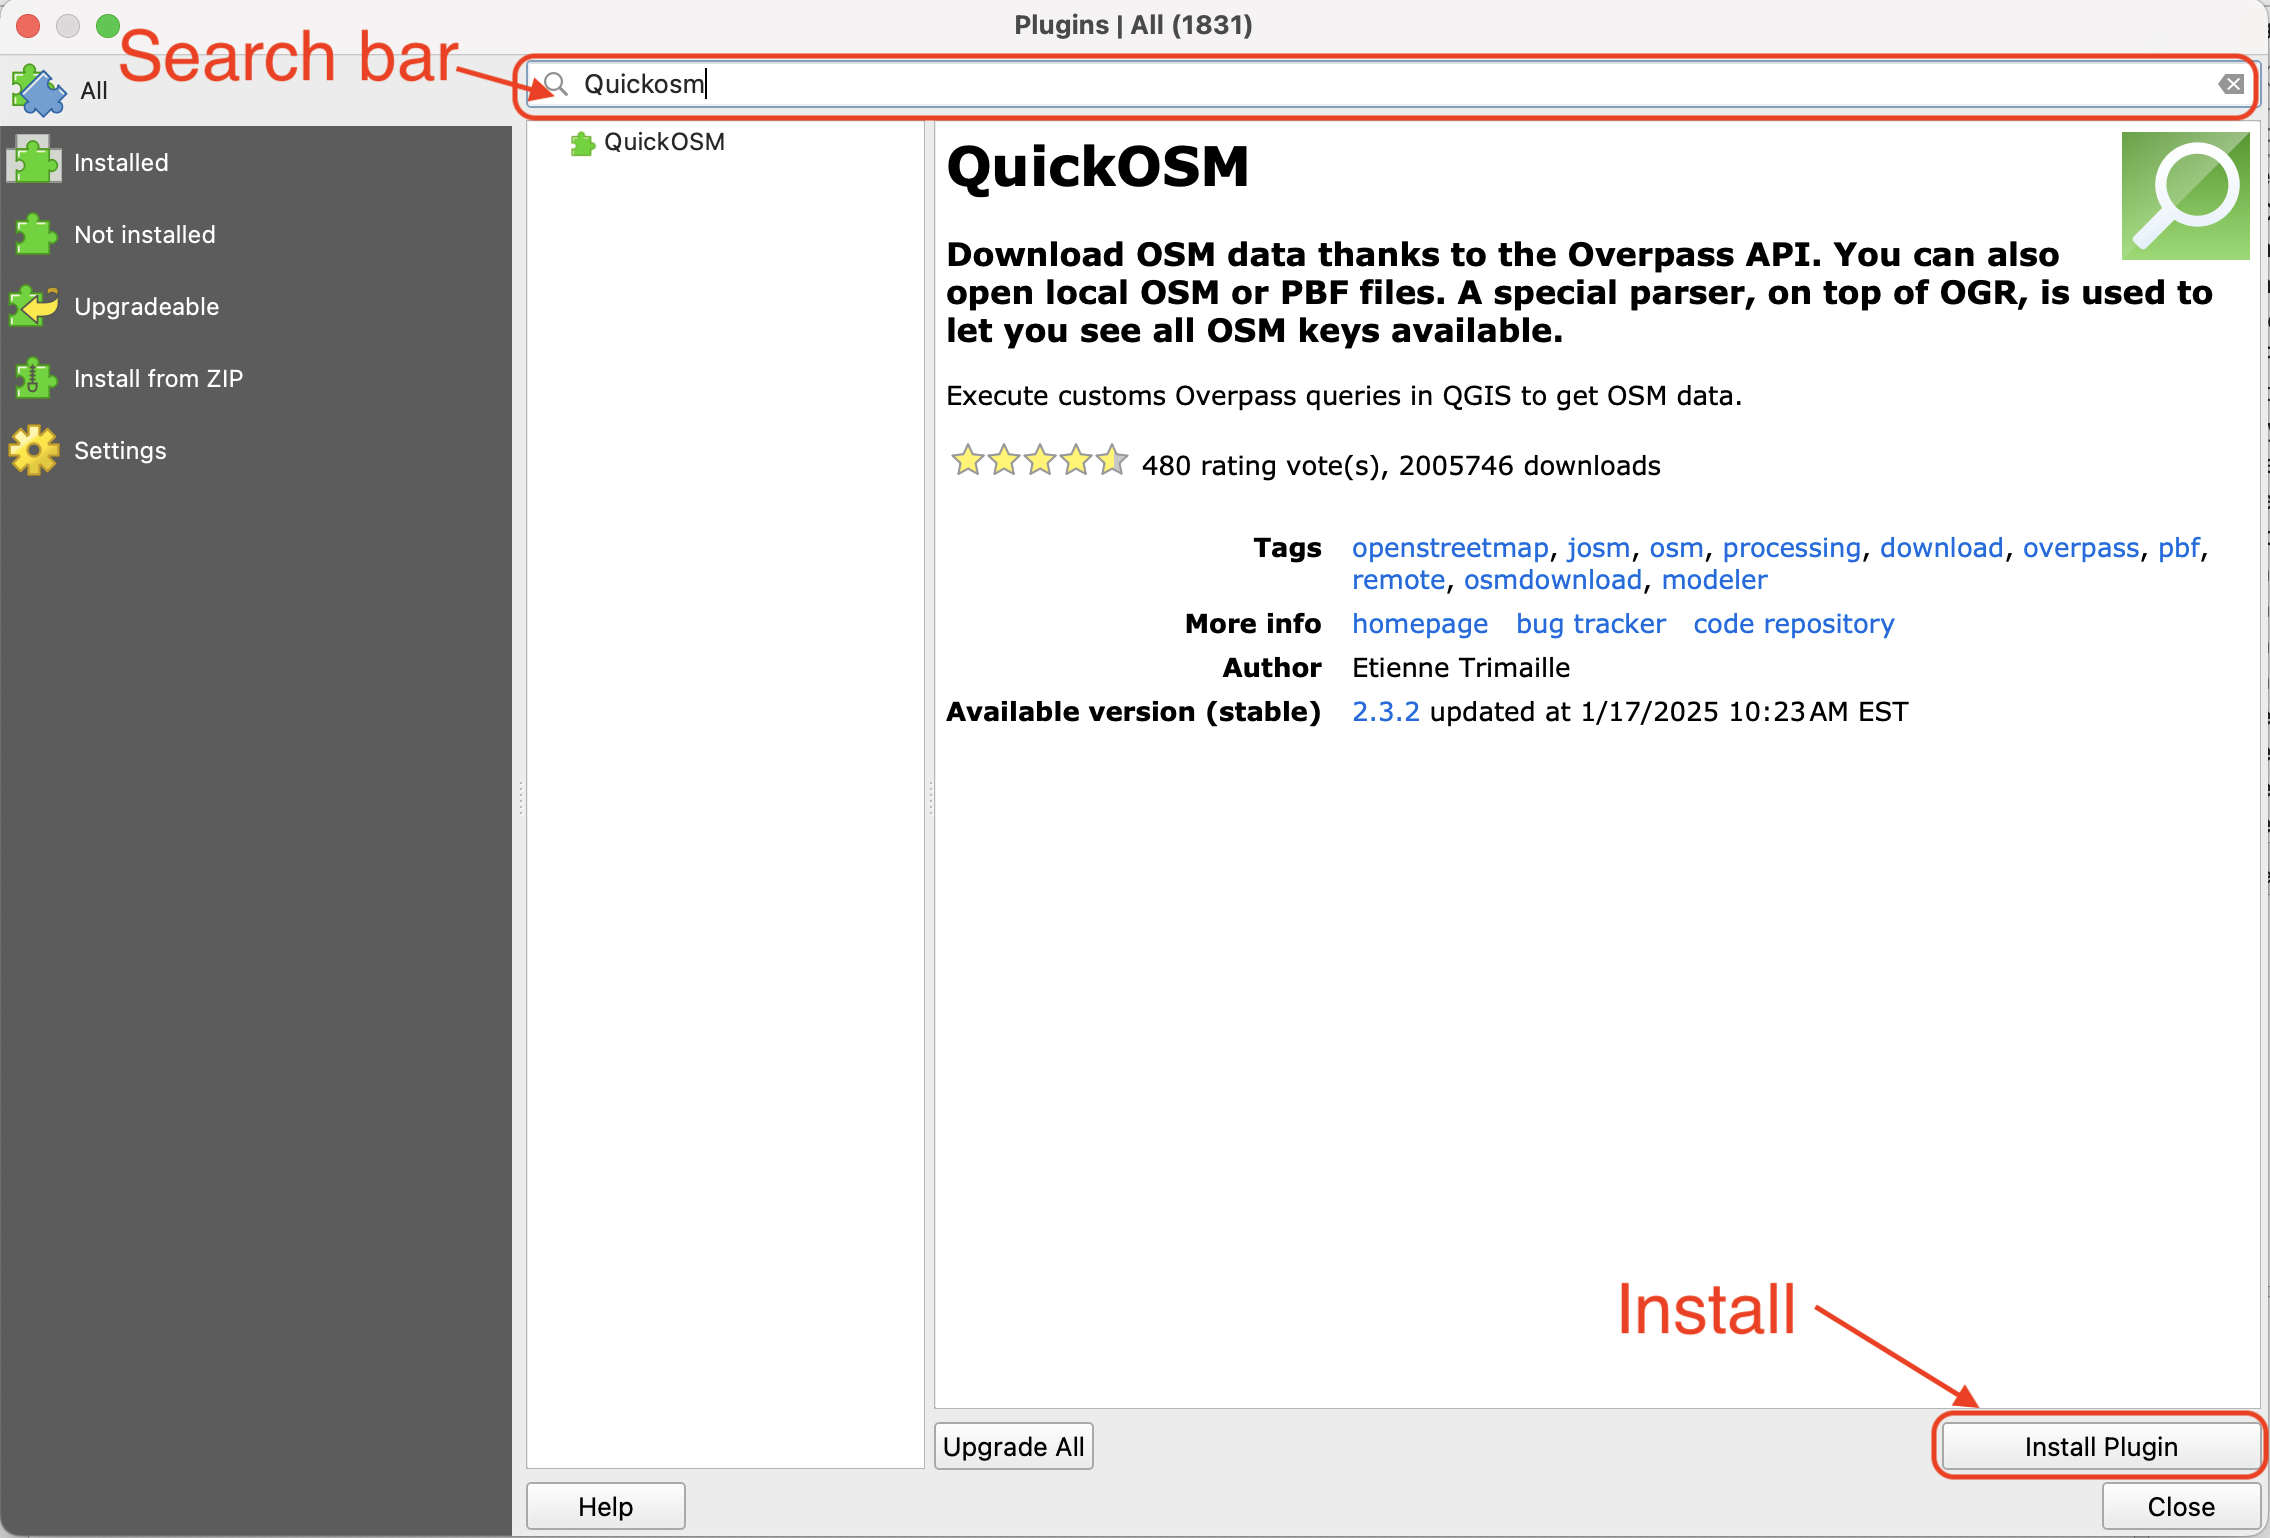
\includegraphics[keepaspectratio]{./images/qgis_inst.png}}

{02} \emph{Build a query to download data}

`QuickOSM' plugin uses
\href{https://wiki.openstreetmap.org/wiki/Overpass_API}{\emph{overpass
API}}, which is is a read-only interface that allows users to query and
extract specific data from the OpenStreetMap (OSM) database using a
custom query language.

To build a custom query:

\begin{itemize}
\tightlist
\item
  Click on the `QuickOSM' button on the toolbar
  
\includegraphics[width=0.04\linewidth,height=\textheight,keepaspectratio]{./images/quickosm.png}
\item
  On the new window:
\end{itemize}

\begin{enumerate}
\def\labelenumi{\arabic{enumi}.}
\tightlist
\item
  Add \texttt{amenity} on the key space and \texttt{parking} on the
  value space.
\item
  Add \texttt{Philadelphia,\ PA} on the `in' space.
\item
  Click on `Run query'.
\end{enumerate}

\pandocbounded{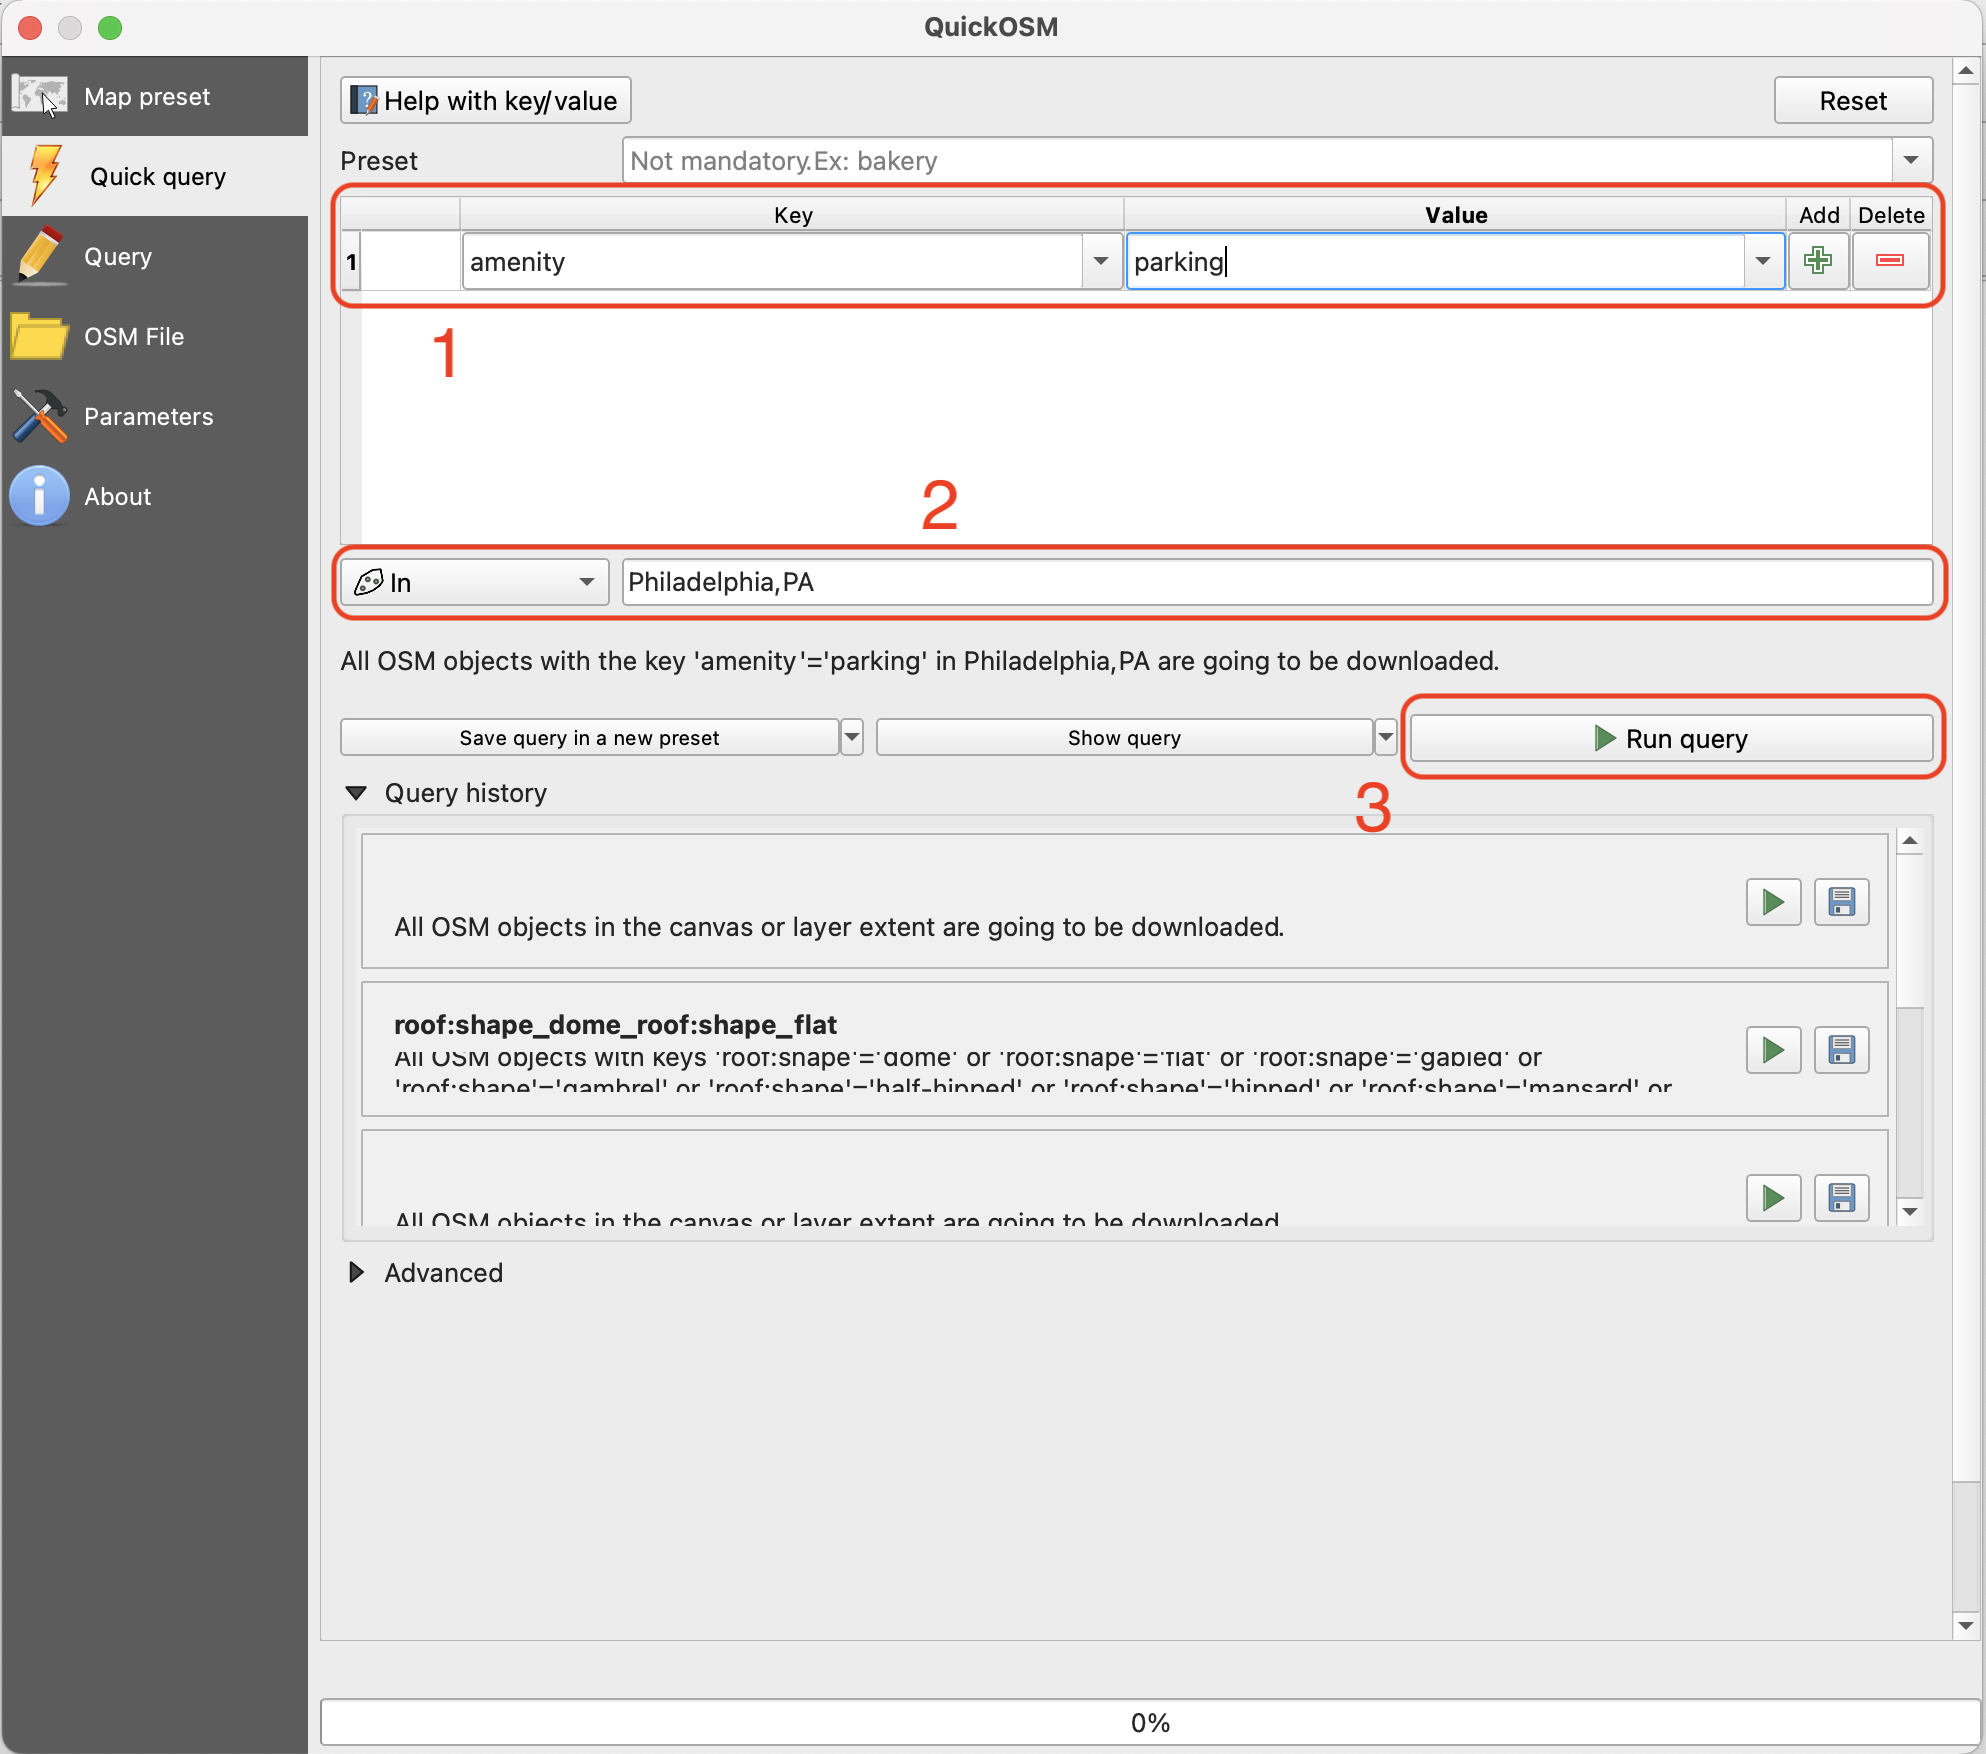
\includegraphics[keepaspectratio]{./images/quick_query.png}}

This will generate a query to retrieve all elements tagged as
`amenity'=`parking' in the city of Philadelphia.

After the download is done, close the `QuickOSM' window and go back to
the map.

\pandocbounded{\includegraphics[keepaspectratio]{./images/qgis_res1.png}}

\begin{tcolorbox}[enhanced jigsaw, opacitybacktitle=0.6, colframe=quarto-callout-note-color-frame, arc=.35mm, leftrule=.75mm, toptitle=1mm, opacityback=0, titlerule=0mm, breakable, colback=white, colbacktitle=quarto-callout-note-color!10!white, toprule=.15mm, bottomtitle=1mm, coltitle=black, title=\textcolor{quarto-callout-note-color}{\faInfo}\hspace{0.5em}{Note}, left=2mm, rightrule=.15mm, bottomrule=.15mm]

\href{https://osm-queries.ldodds.com/tutorial/index.html}{\textbf{Learn
more}} on how overpass queries work in this tutorial.

\end{tcolorbox}

{03} \emph{Save and style the layers}

The data downloaded is stored as a temporary file in your system.

\pandocbounded{\includegraphics[keepaspectratio]{./images/save1.png}}

If you want to use it further from this session in QGIS you first need
to save the files in your system.

To do so:

\begin{enumerate}
\def\labelenumi{\arabic{enumi}.}
\tightlist
\item
  Right click on the name of the layer you want to save.
\item
  Click on the option `Make permanent' or `Export' and then `Save
  feature as\ldots{}'.
\item
  In the new window, select the format for your file, a name and, a
  location.
\item
  Then click `OK'.
\end{enumerate}

\pandocbounded{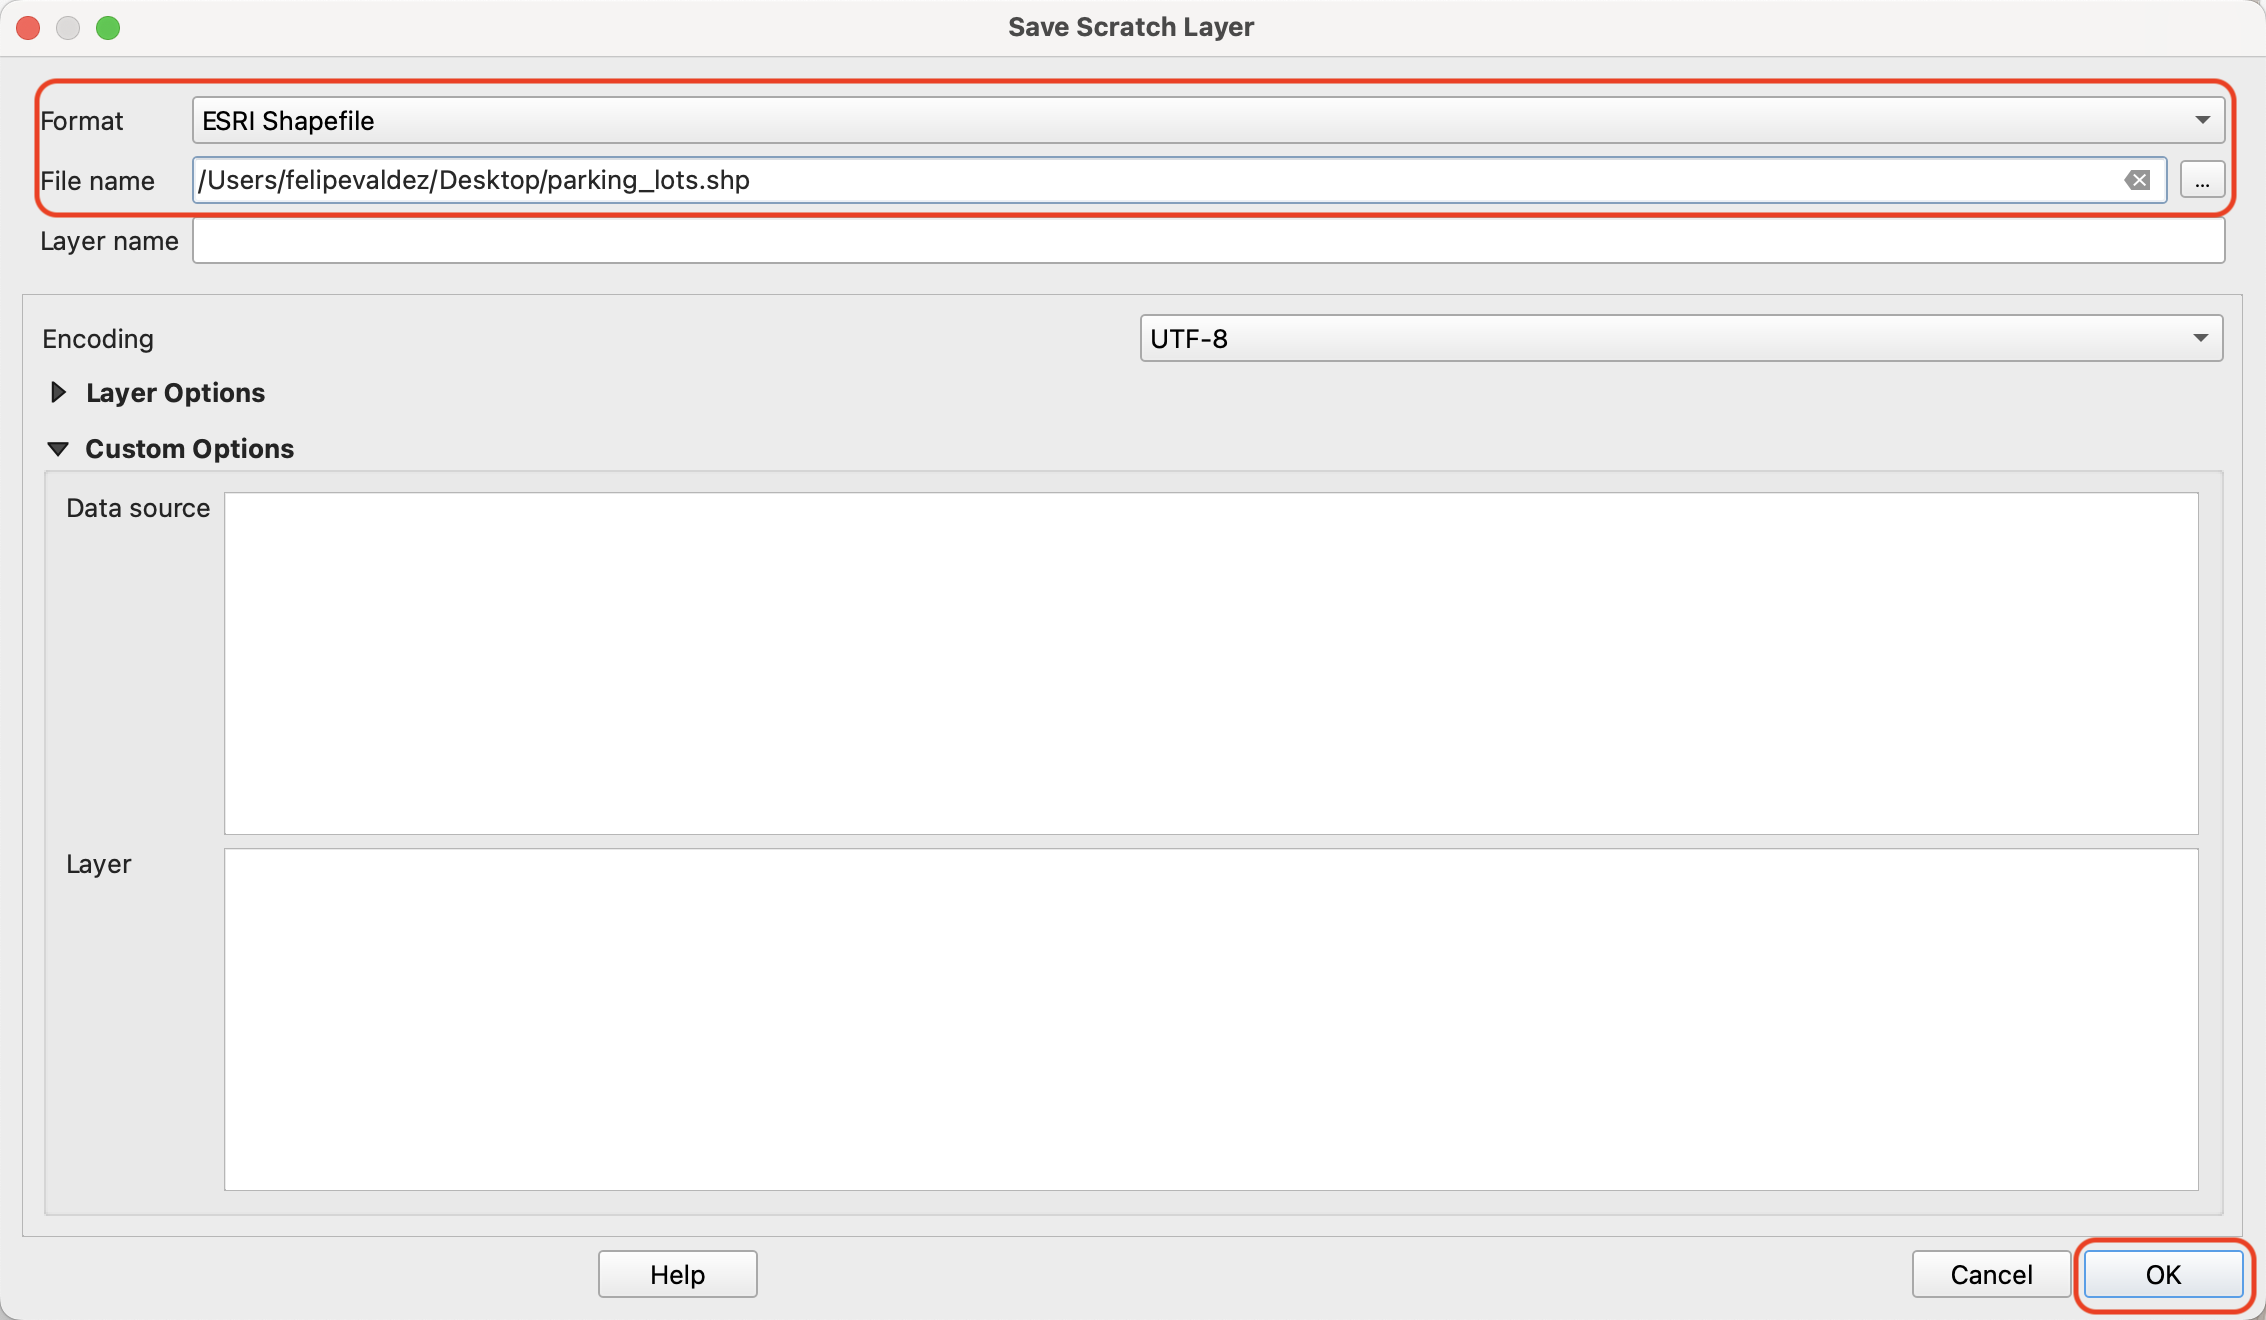
\includegraphics[keepaspectratio]{./images/save2.png}}

\begin{tcolorbox}[enhanced jigsaw, opacitybacktitle=0.6, colframe=quarto-callout-caution-color-frame, arc=.35mm, leftrule=.75mm, toptitle=1mm, opacityback=0, titlerule=0mm, breakable, colback=white, colbacktitle=quarto-callout-caution-color!10!white, toprule=.15mm, bottomtitle=1mm, coltitle=black, title=\textcolor{quarto-callout-caution-color}{\faFire}\hspace{0.5em}{Go further}, left=2mm, rightrule=.15mm, bottomrule=.15mm]

There are other options to download data usin `QuickOSM' plugin.

You can try \emph{preset} downloads, play around with different
combinations of \texttt{key} and \texttt{value}, or download all data
for a specific area. To download all data for a specific area, take into
account that the amount of data can exceed your system capacity. Start
downloading smaller areas to test.

For example, zoom in to a neighborhood or block, then in the `QuickOSM'
plugin window use `Canvas Extent' then execute the query.

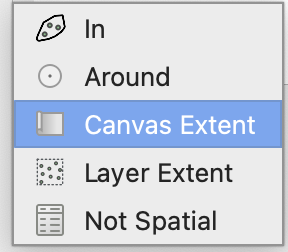
\includegraphics[width=0.2\linewidth,height=\textheight,keepaspectratio]{./images/canvas.png}

\end{tcolorbox}

\subsection{From Overture Maps}\label{from-overture-maps}

To download data from Overture Maps directly to QGIS we are going to use
two plugins:

\href{https://plugins.qgis.org/plugins/qduckdb/}{QduckDB} and
\href{https://plugins.qgis.org/plugins/qgis_plugin_gpq_downloader/}{GeoParquet
Downloader}.

Follow the steps forward to download data directly to QGIS.

{01} \emph{Install DuckDB plugin}

Open QGIS.

On the top menu bar click on `Plugins' and then on `Manage and Install
Plugins'.

\pandocbounded{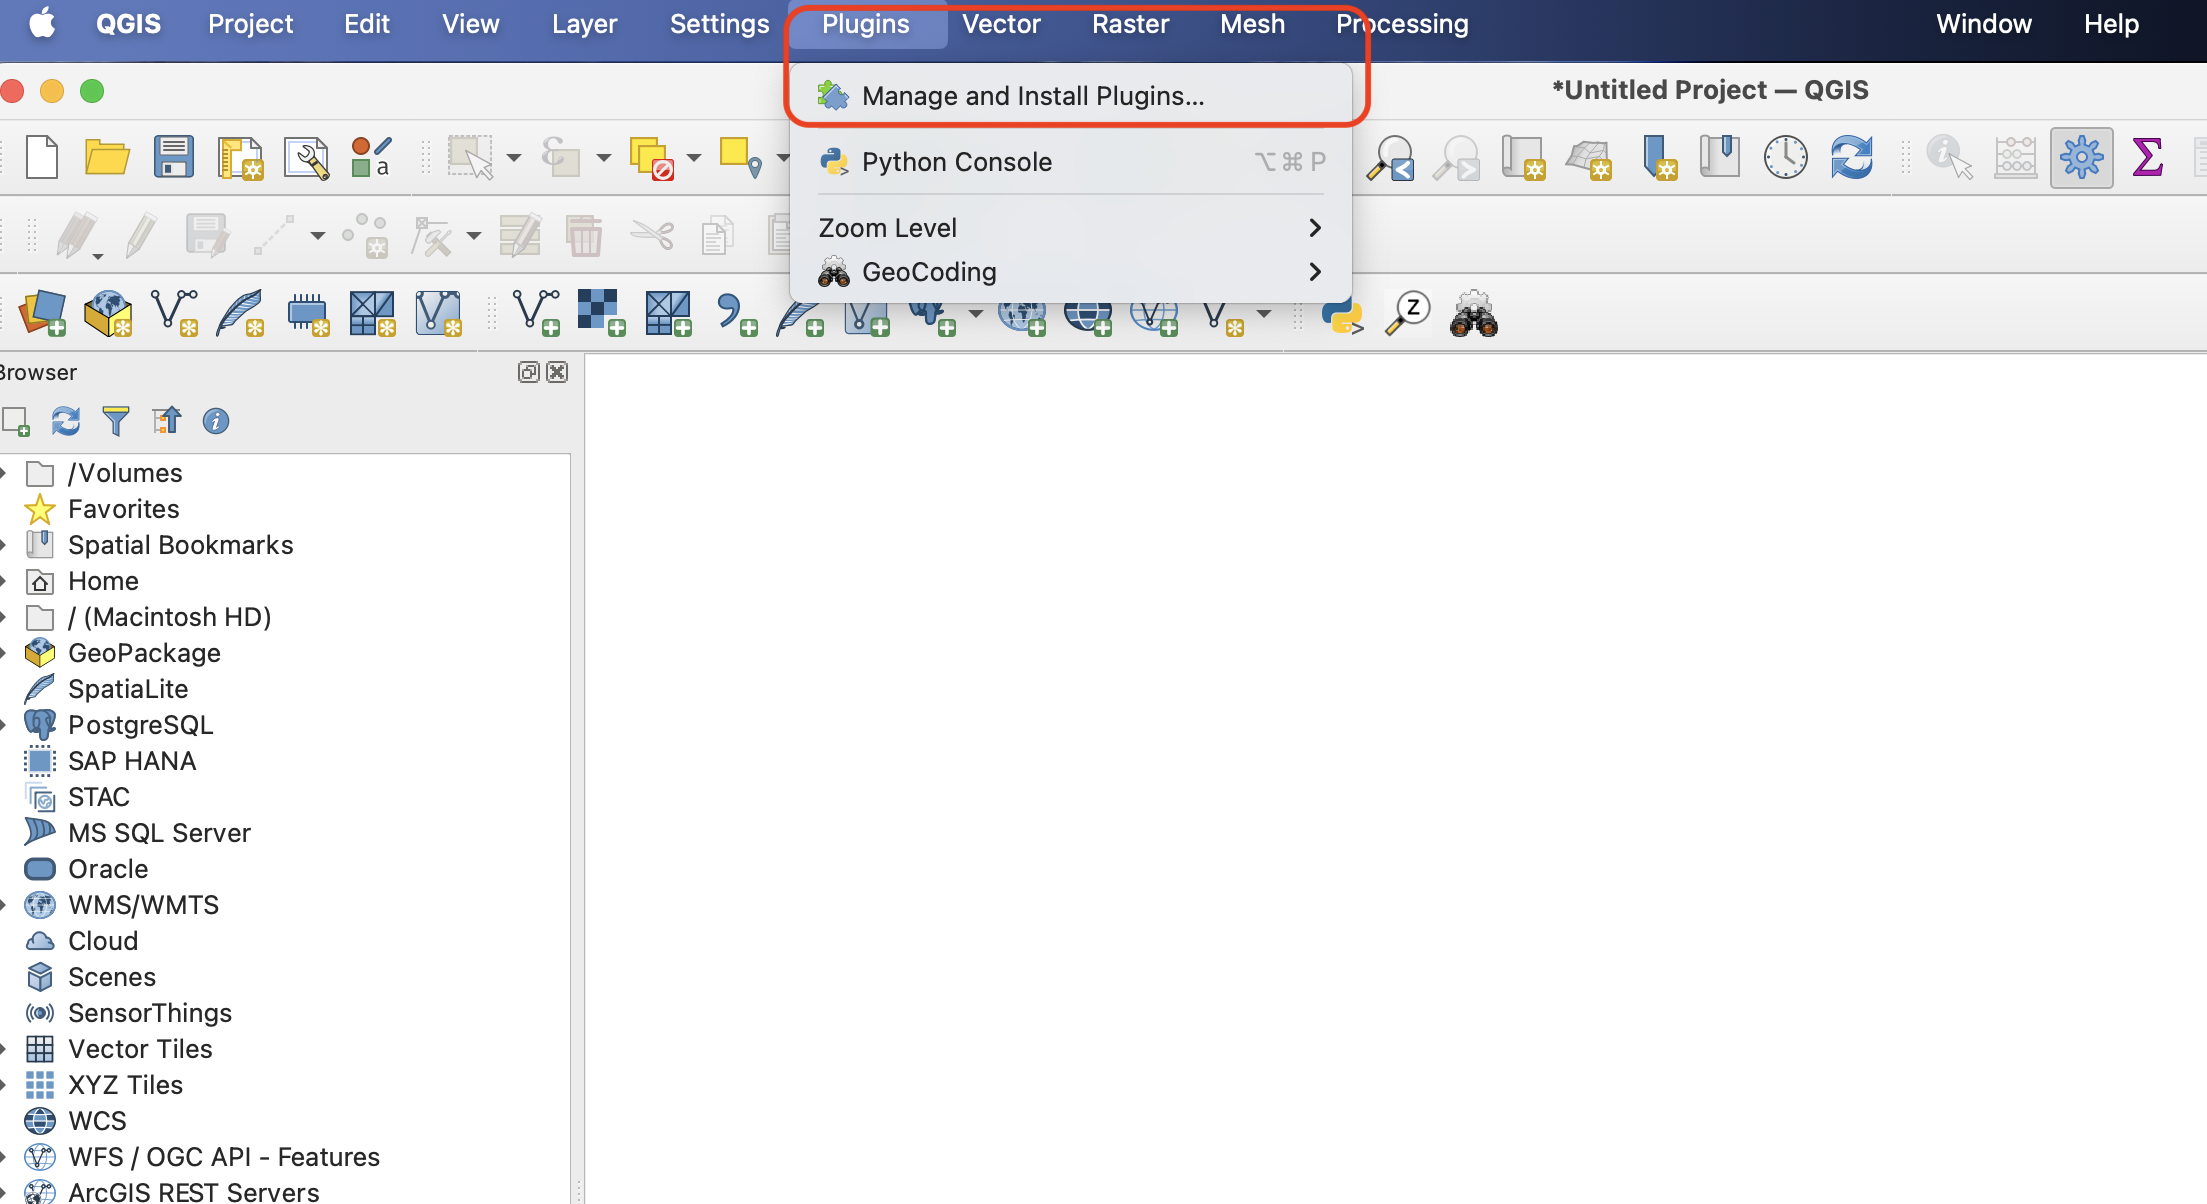
\includegraphics[keepaspectratio]{./images/qgis_mn.png}}

On the new window, in the search bar type \texttt{qduckdb}, then click
on `Install plugin'. Once installed, close the plugins manager window.

\pandocbounded{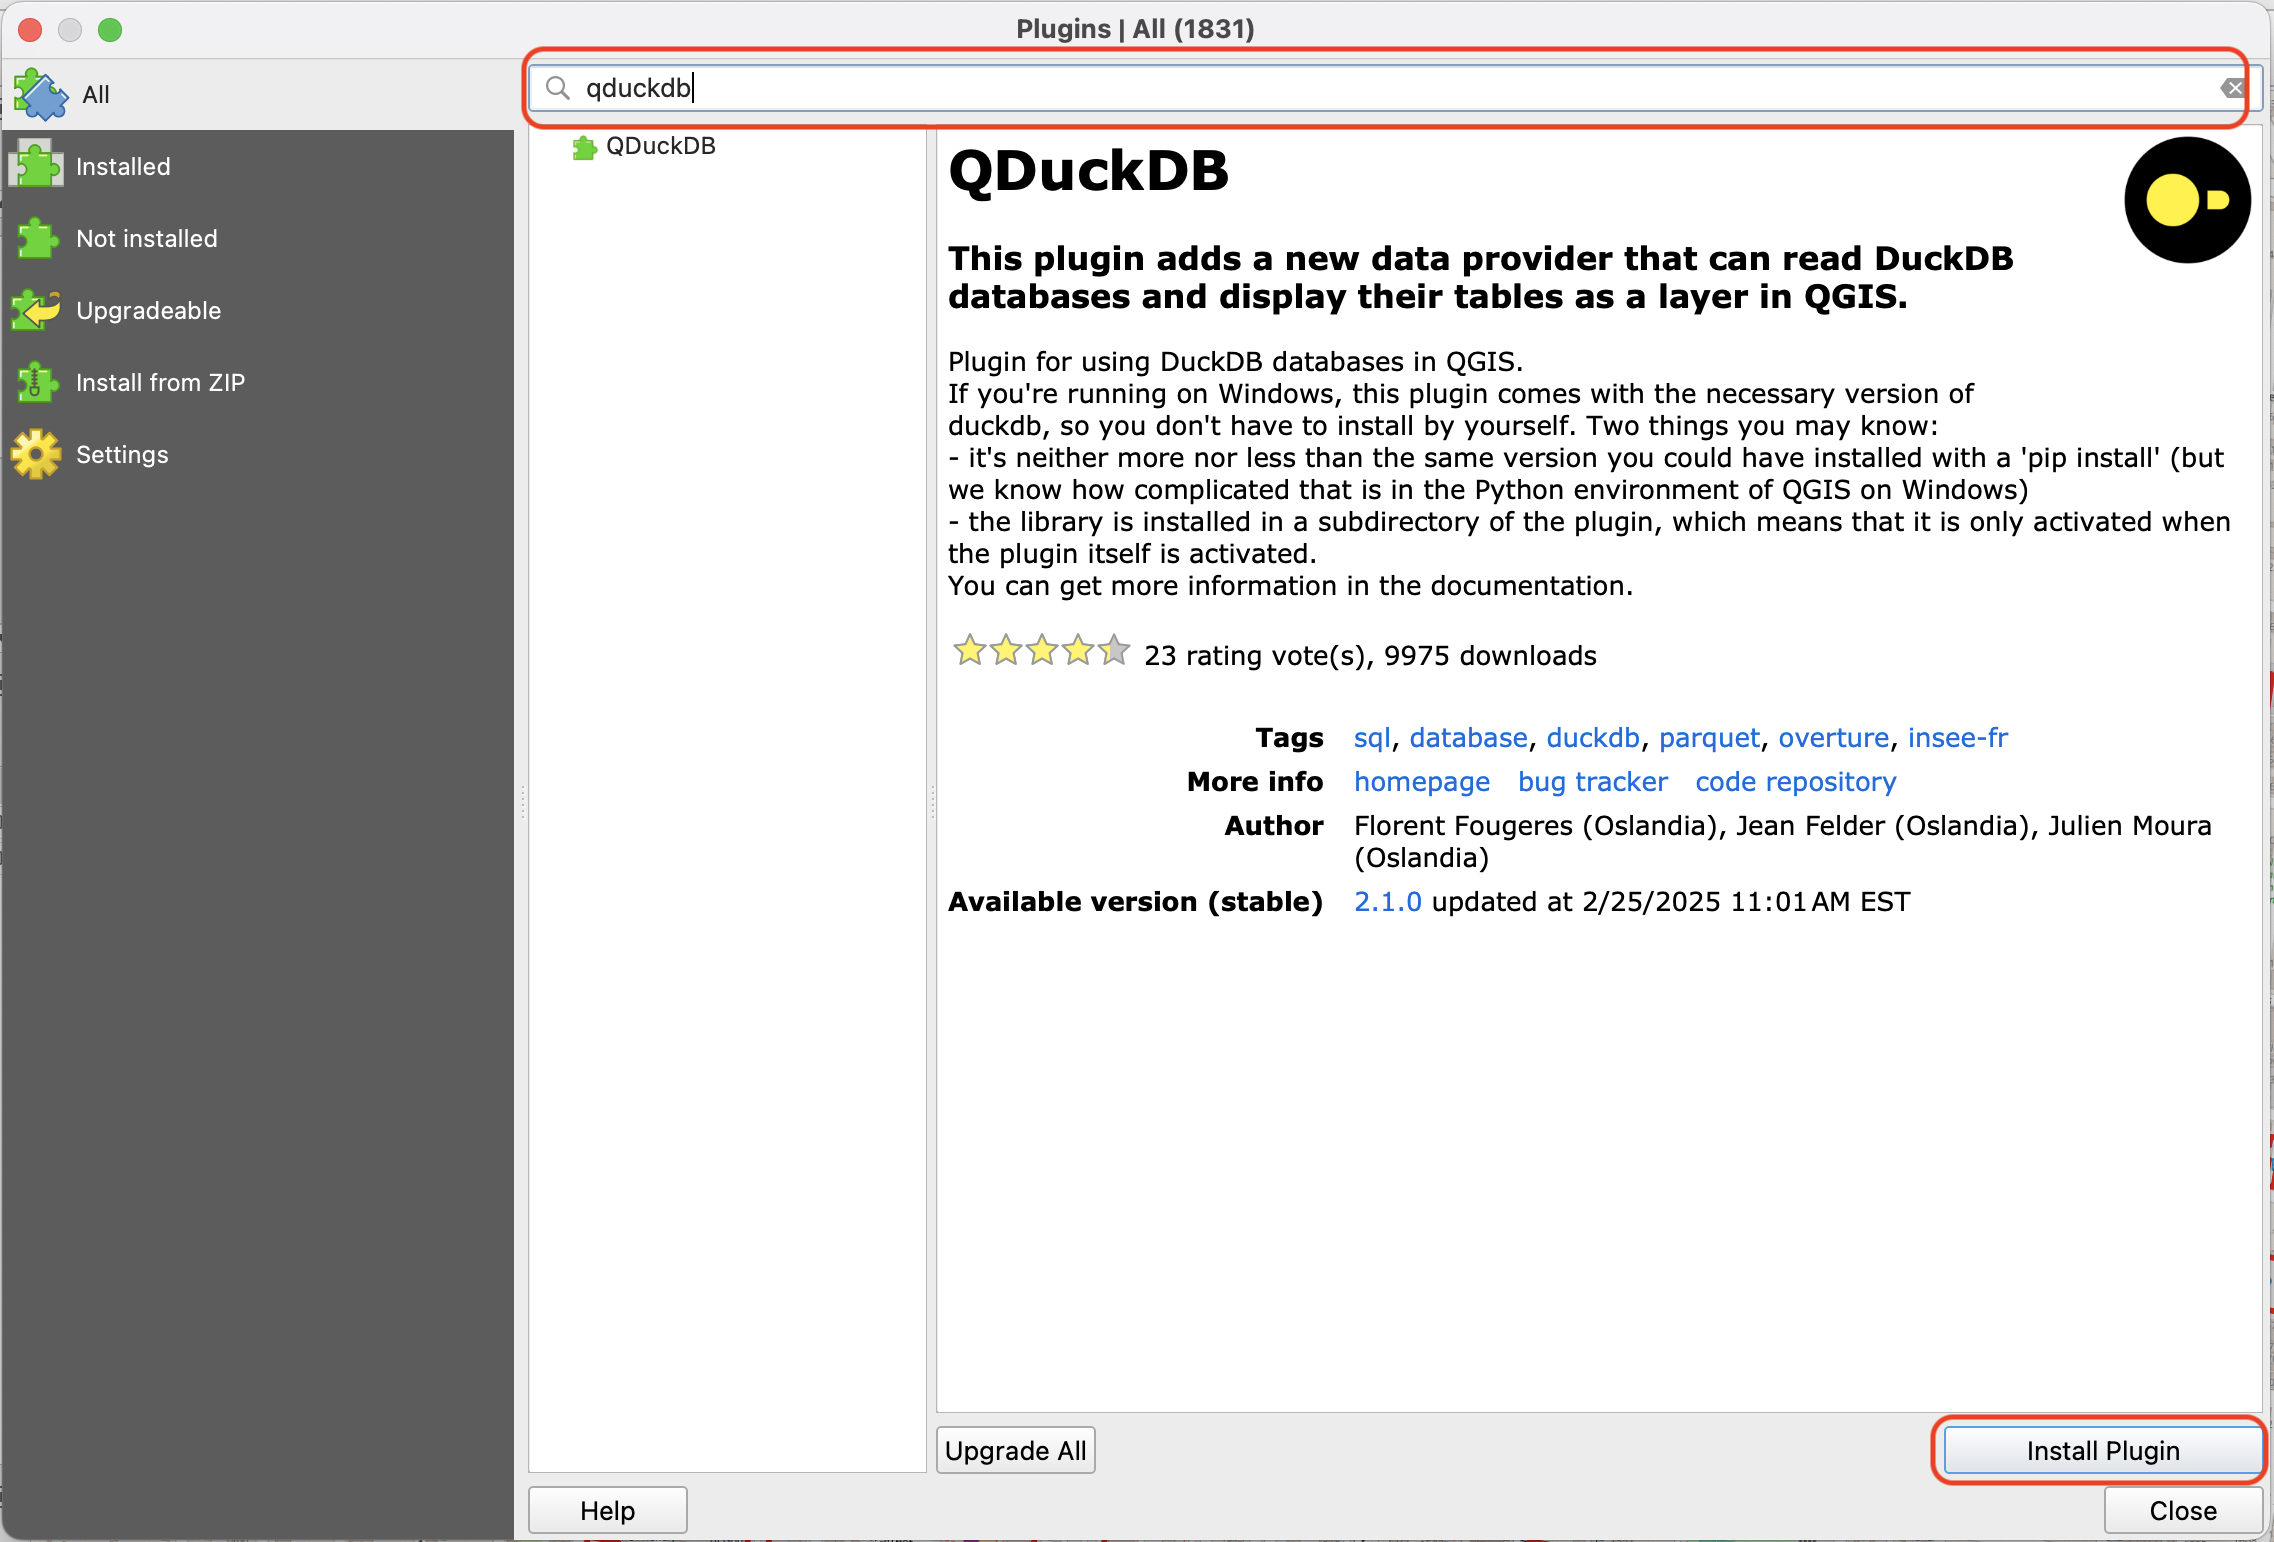
\includegraphics[keepaspectratio]{./images/qgis_inst1.png}}
Go back to the Plugins amanger and check that the `QduckDB' plugin is
activated (with a check mark).

\pandocbounded{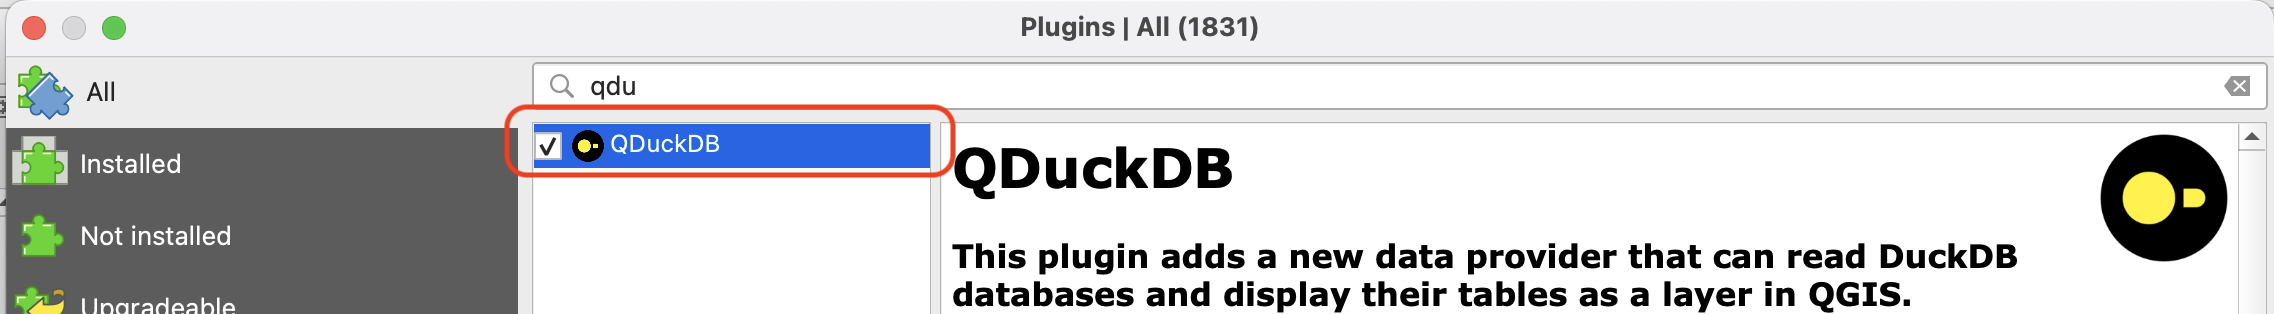
\includegraphics[keepaspectratio]{./images/qgis_check.png}}
If not, check the box.

If you get an error message, follow the instructions in the following
warining box.

\begin{tcolorbox}[enhanced jigsaw, opacitybacktitle=0.6, colframe=quarto-callout-warning-color-frame, arc=.35mm, leftrule=.75mm, toptitle=1mm, opacityback=0, titlerule=0mm, breakable, colback=white, colbacktitle=quarto-callout-warning-color!10!white, toprule=.15mm, bottomtitle=1mm, coltitle=black, title=\textcolor{quarto-callout-warning-color}{\faExclamationTriangle}\hspace{0.5em}{Warning!}, left=2mm, rightrule=.15mm, bottomrule=.15mm]

Depending on the oprating system you are using, the QduckDB plugin will
need some extra steps to function correctly.

On MacOS:

\begin{enumerate}
\def\labelenumi{\arabic{enumi}.}
\tightlist
\item
  Open the terminal app
  
\includegraphics[width=0.06\linewidth,height=\textheight,keepaspectratio]{opengeodata_files/mediabag/Terminalicon2.png}
\item
  Type the following:
\end{enumerate}

\begin{Shaded}
\begin{Highlighting}[]
\ExtensionTok{/Applications/QGIS.app/Contents/MacOS/bin/python3.9} \AttributeTok{{-}m}\NormalTok{ pip install }\StringTok{"duckdb==1.2.0"}
\end{Highlighting}
\end{Shaded}

\begin{enumerate}
\def\labelenumi{\arabic{enumi}.}
\setcounter{enumi}{2}
\tightlist
\item
  In terminal, locate and open the plugin file by typing:
\end{enumerate}

\begin{Shaded}
\begin{Highlighting}[]
\ExtensionTok{open}\NormalTok{ \textasciitilde{}/Library/}\StringTok{\textquotesingle{}Application Support\textquotesingle{}}\NormalTok{/QGIS/QGIS3/profiles/default/python/plugins/qduckdb/gui/}
\end{Highlighting}
\end{Shaded}

\begin{enumerate}
\def\labelenumi{\arabic{enumi}.}
\setcounter{enumi}{3}
\tightlist
\item
  Open the file \texttt{dlg\_add\_duckdb\_layer.py} on a text editor
  app.
  \pandocbounded{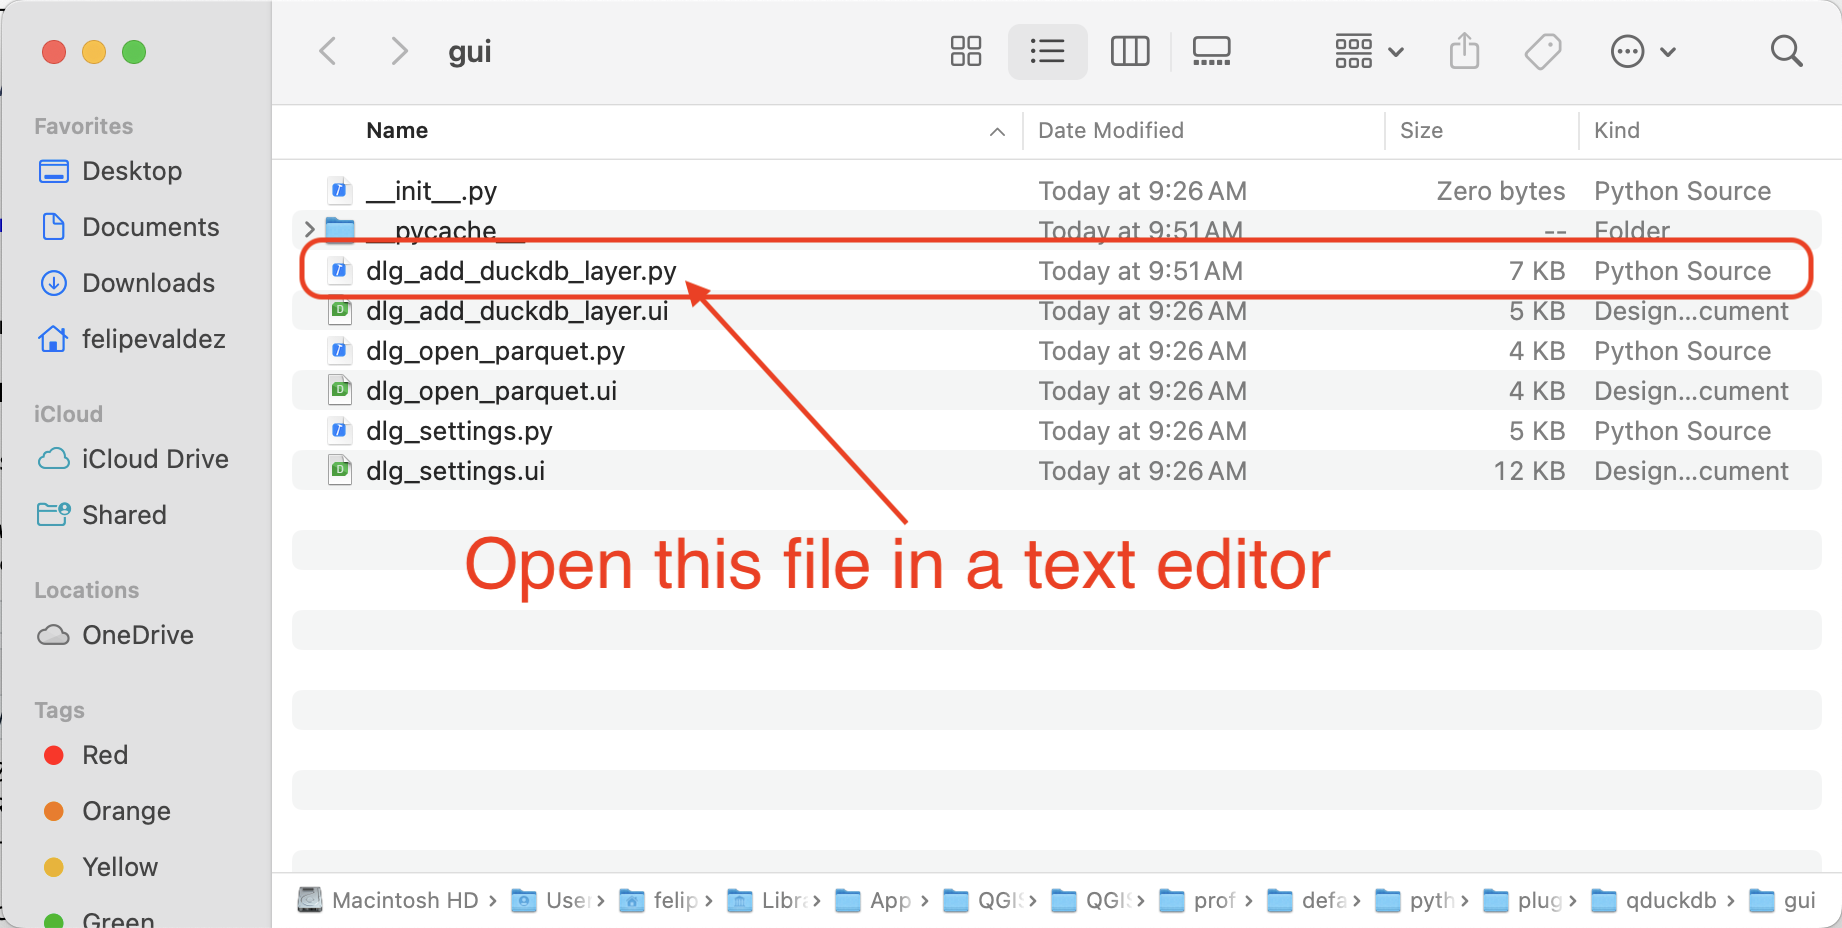
\includegraphics[keepaspectratio]{./images/qgis_open.png}}
\item
  Add the followin to line 3:
\end{enumerate}

\begin{Shaded}
\begin{Highlighting}[]
\ImportTok{import}\NormalTok{ typing}
\end{Highlighting}
\end{Shaded}

\begin{enumerate}
\def\labelenumi{\arabic{enumi}.}
\setcounter{enumi}{5}
\tightlist
\item
  Replace the text on line 89 with:
\end{enumerate}

\begin{Shaded}
\begin{Highlighting}[]
\KeywordTok{def}\NormalTok{ db\_path(}\VariableTok{self}\NormalTok{) }\OperatorTok{{-}\textgreater{}}\NormalTok{ typing.Union[Path, }\VariableTok{None}\NormalTok{]:}
\end{Highlighting}
\end{Shaded}

\begin{enumerate}
\def\labelenumi{\arabic{enumi}.}
\setcounter{enumi}{6}
\tightlist
\item
  Save the file.
\item
  Reopen QGIS.
\item
  Activate QduckDB plugin.
\end{enumerate}

\href{https://oslandia.gitlab.io/qgis/qduckdb/usage/installation.html}{Here
you can find instructions for other OS.}

\end{tcolorbox}

{02} \emph{Install GeoParquet Downloader plugin}

On the top menu bar click on `Plugins' and then on `Manage and Install
Plugins'.

\pandocbounded{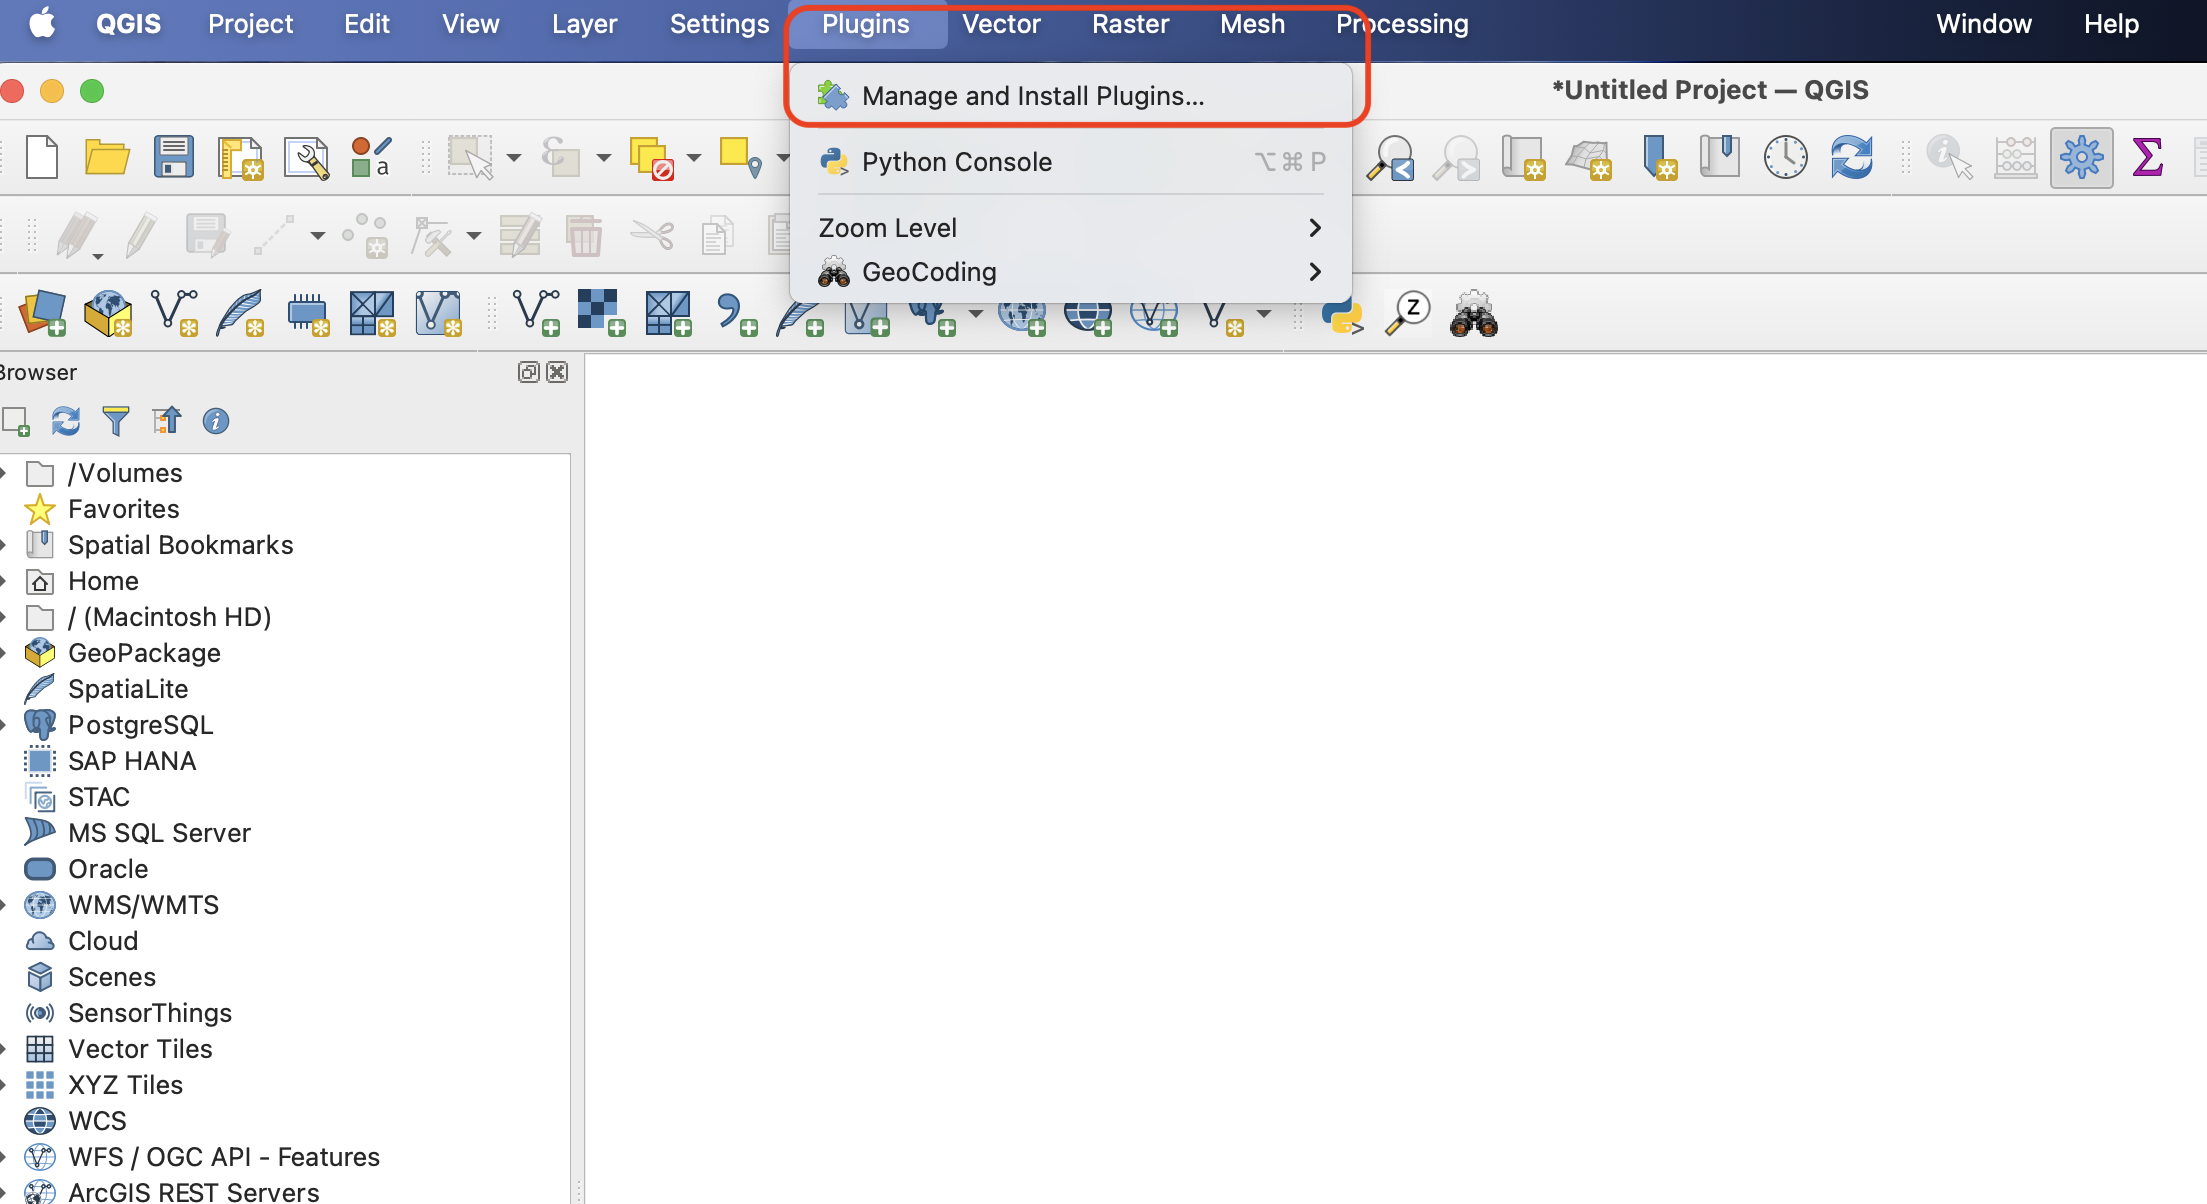
\includegraphics[keepaspectratio]{./images/qgis_mn.png}}

On the new window, in the search bar type
\texttt{geoparquet\ downloader}, then click on `Install plugin'. Once
installed, close the plugins manager window.

\pandocbounded{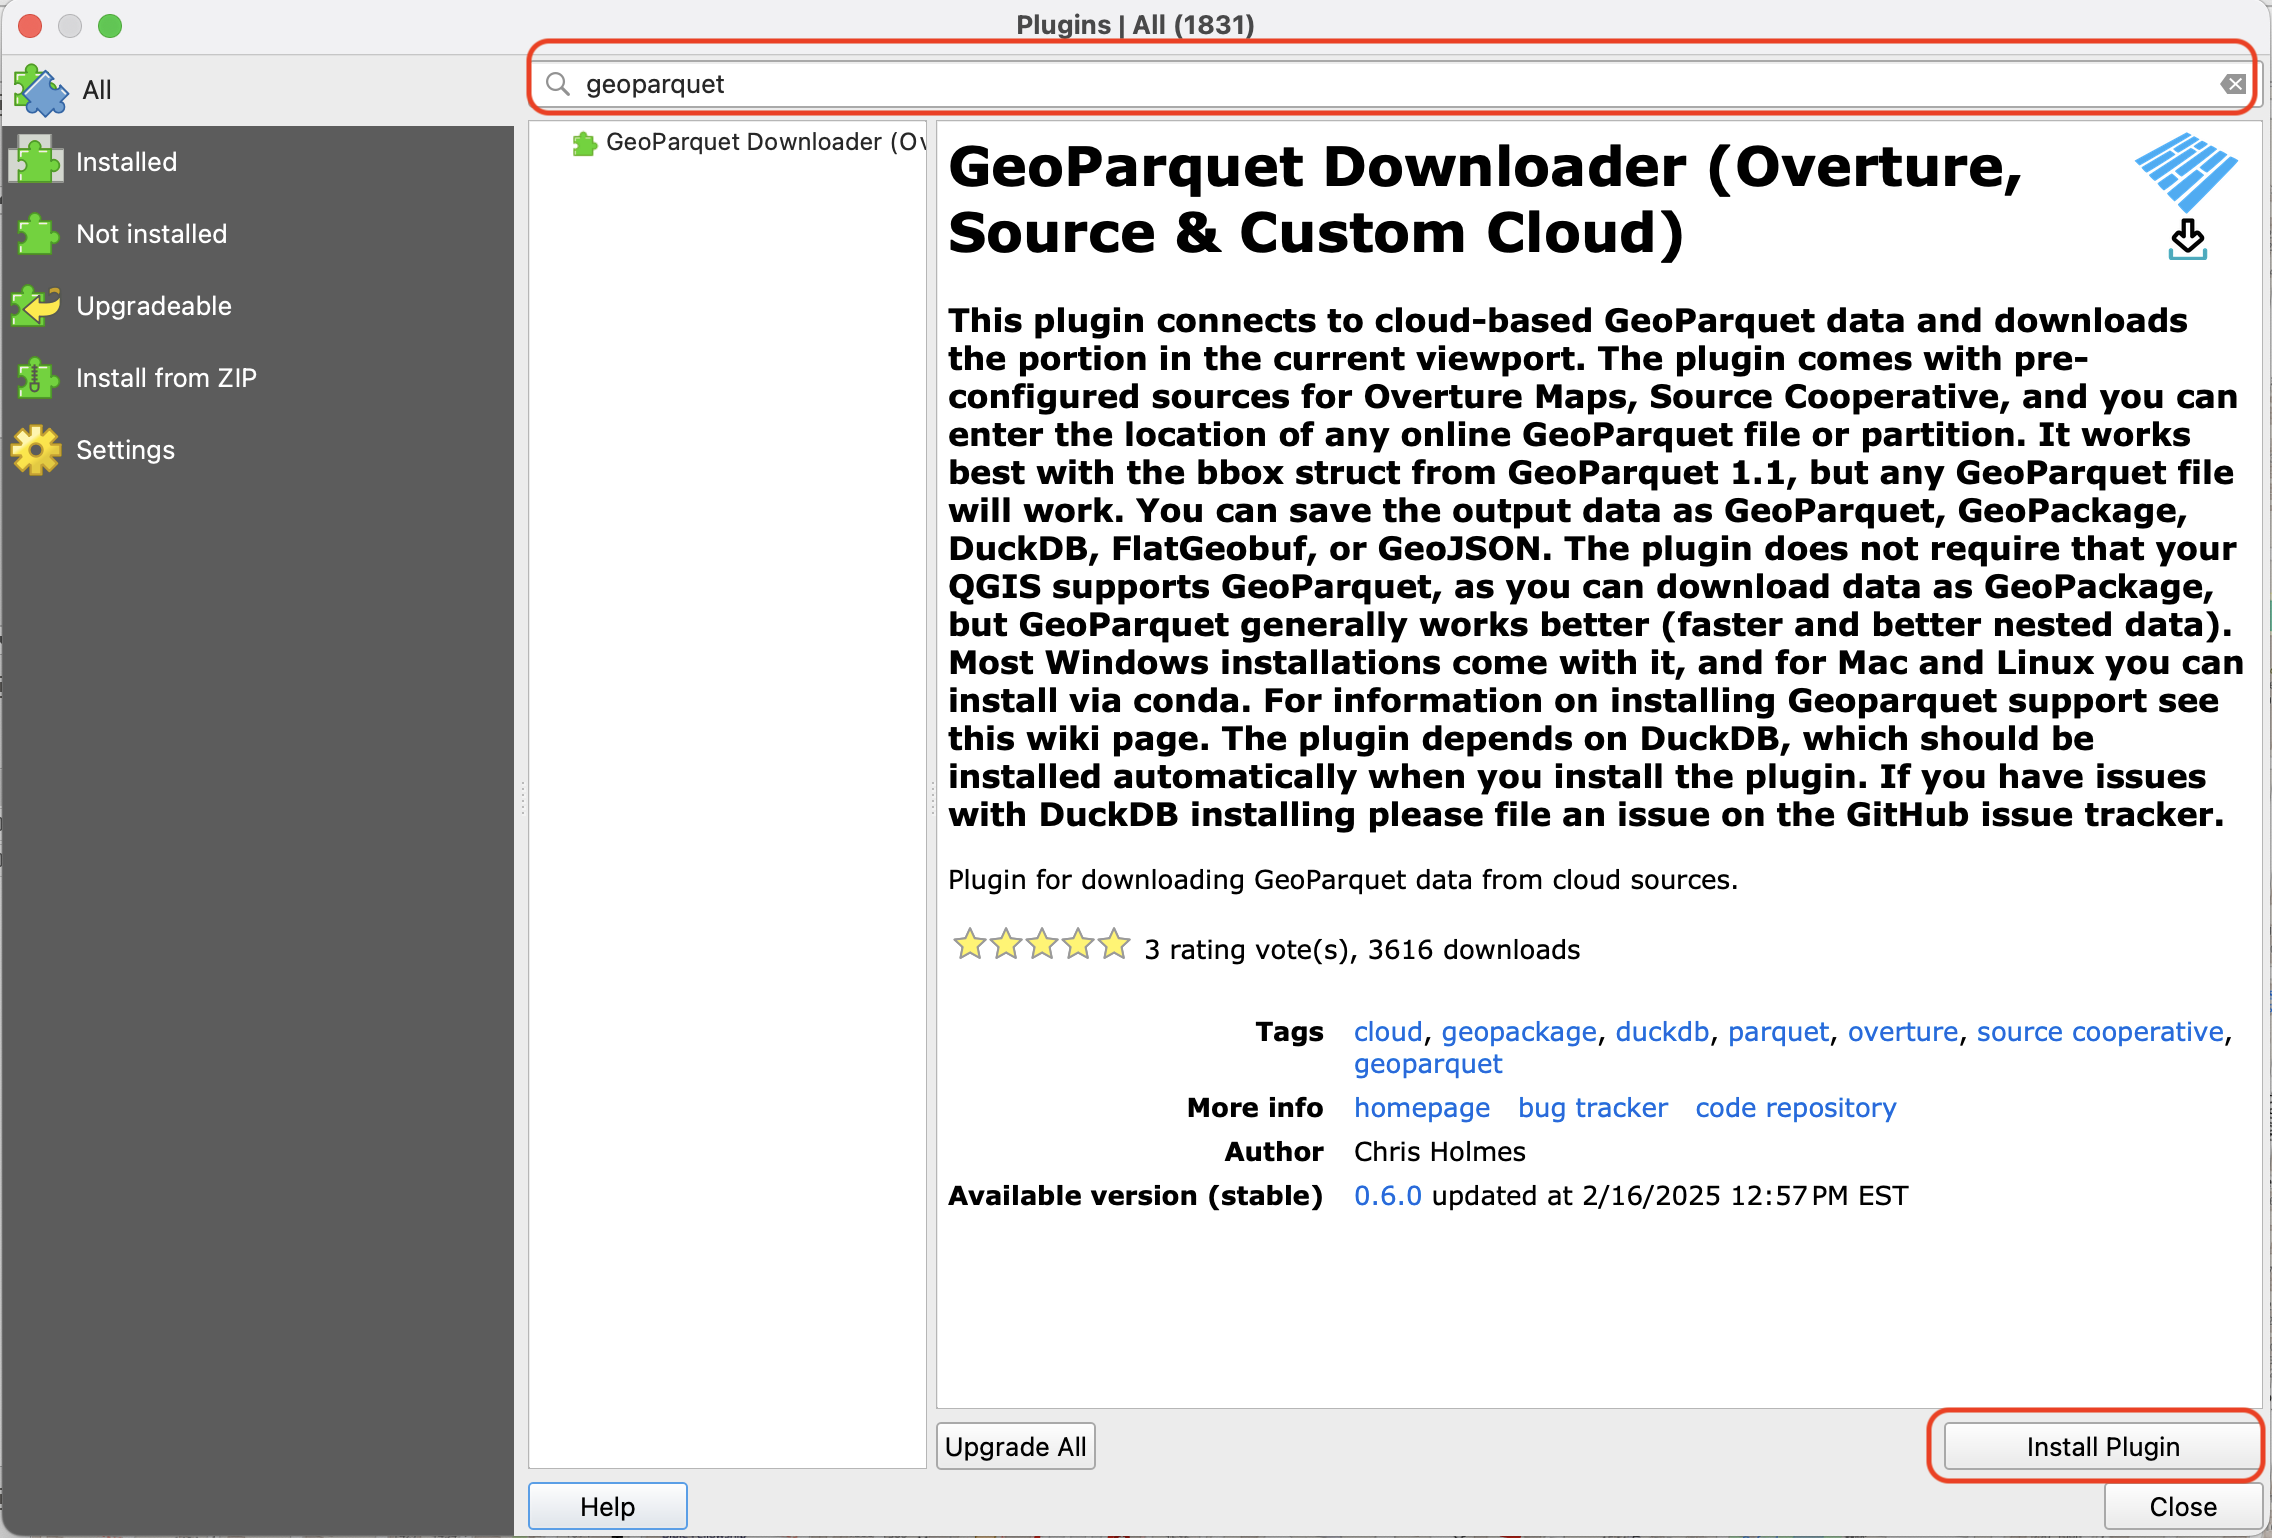
\includegraphics[keepaspectratio]{./images/qgis_inst2.png}}

You should see the following icons on your tool bar
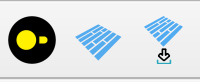
\includegraphics[width=0.1\linewidth,height=\textheight,keepaspectratio]{./images/new_icons.png}

If not, right click on any empty space on the tool bar and activate the
`Plugins toolbar'.
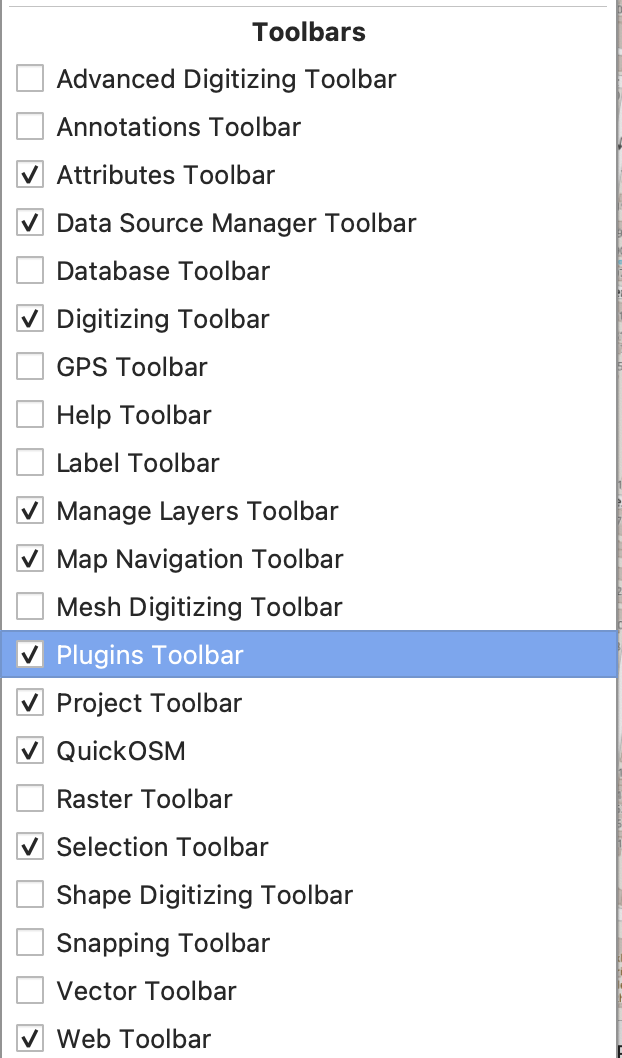
\includegraphics[width=0.2\linewidth,height=\textheight,keepaspectratio]{./images/toolbar.png}

{03} \emph{Select the data source and type to download}

\begin{tcolorbox}[enhanced jigsaw, opacitybacktitle=0.6, colframe=quarto-callout-note-color-frame, arc=.35mm, leftrule=.75mm, toptitle=1mm, opacityback=0, titlerule=0mm, breakable, colback=white, colbacktitle=quarto-callout-note-color!10!white, toprule=.15mm, bottomtitle=1mm, coltitle=black, title=\textcolor{quarto-callout-note-color}{\faInfo}\hspace{0.5em}{Note}, left=2mm, rightrule=.15mm, bottomrule=.15mm]

\href{https://geoparquet.org/}{GeoParquet} is a geospatial extension of
`Apache Parquet' format that efficiently stores geographic data in a
columnar structure. It provides optimized compression, native support
for geometries (points, lines, polygons), and includes spatial metadata
like coordinate reference systems.

\end{tcolorbox}

\begin{itemize}
\tightlist
\item
  Click on the `Download GeoParquet Data' button on the toolbar
  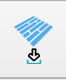
\includegraphics[width=0.04\linewidth,height=\textheight,keepaspectratio]{./images/geop_but.png}
\item
  In the new window, select the source `Overture Maps' and the types you
  want to download.
  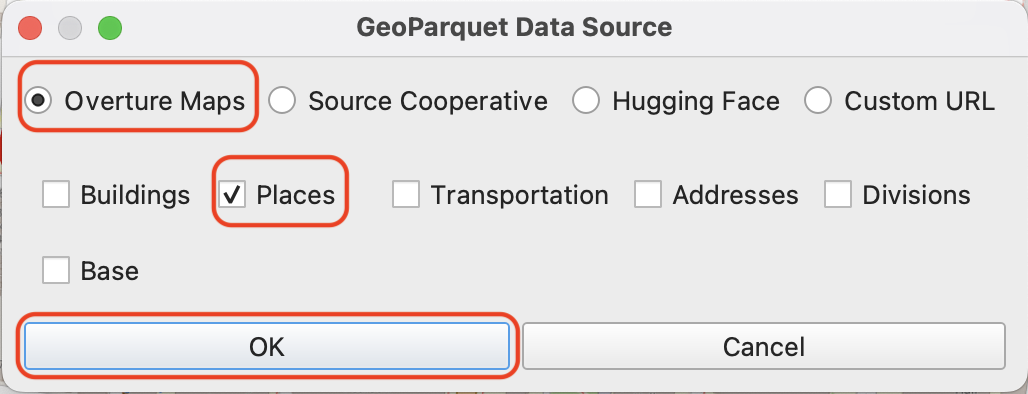
\includegraphics[width=0.5\linewidth,height=\textheight,keepaspectratio]{./images/geop_source.png}
\item
  Set a directory and name where you want to save the file.
\end{itemize}

\begin{tcolorbox}[enhanced jigsaw, opacitybacktitle=0.6, colframe=quarto-callout-warning-color-frame, arc=.35mm, leftrule=.75mm, toptitle=1mm, opacityback=0, titlerule=0mm, breakable, colback=white, colbacktitle=quarto-callout-warning-color!10!white, toprule=.15mm, bottomtitle=1mm, coltitle=black, title=\textcolor{quarto-callout-warning-color}{\faExclamationTriangle}\hspace{0.5em}{Warning!}, left=2mm, rightrule=.15mm, bottomrule=.15mm]

The `GeoParquet Downloader' will download data for the current map
extent. Be sure to limite the view to a local area to avoid saturating
the download process.

\end{tcolorbox}

Once the download is complete you should see a message like this:
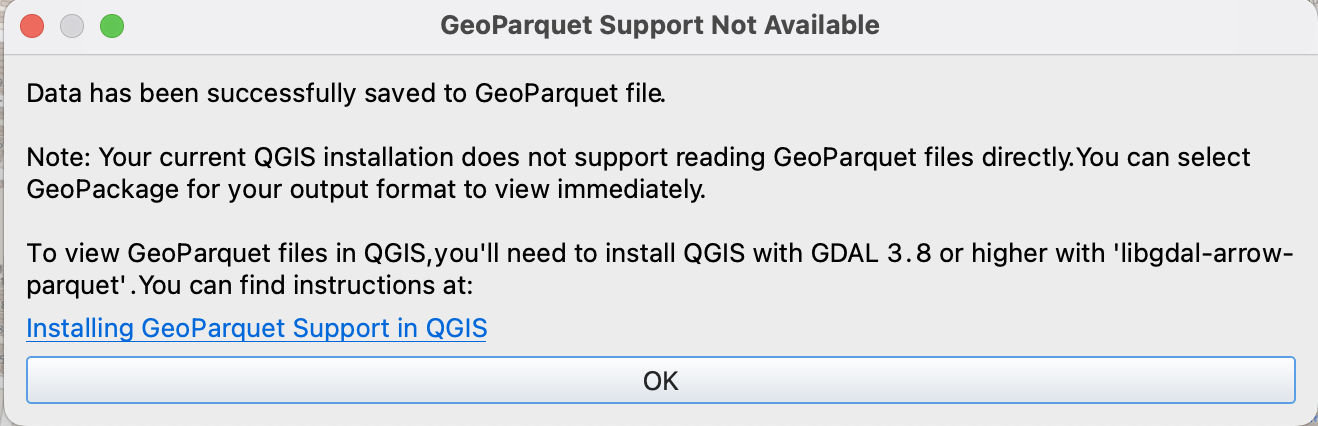
\includegraphics[width=0.7\linewidth,height=\textheight,keepaspectratio]{./images/geop_mess.png}

{04} \emph{Open the downloaded data}

\begin{itemize}
\tightlist
\item
  Click on the `Open Parquet with DuckDB' button on the toolbar
  
\includegraphics[width=0.04\linewidth,height=\textheight,keepaspectratio]{./images/duck_open.png}
\item
  Point to the file you downloaded in the previous step and set
  EPSG:4326 as the CRS.
\item
  Click `Open'
\end{itemize}

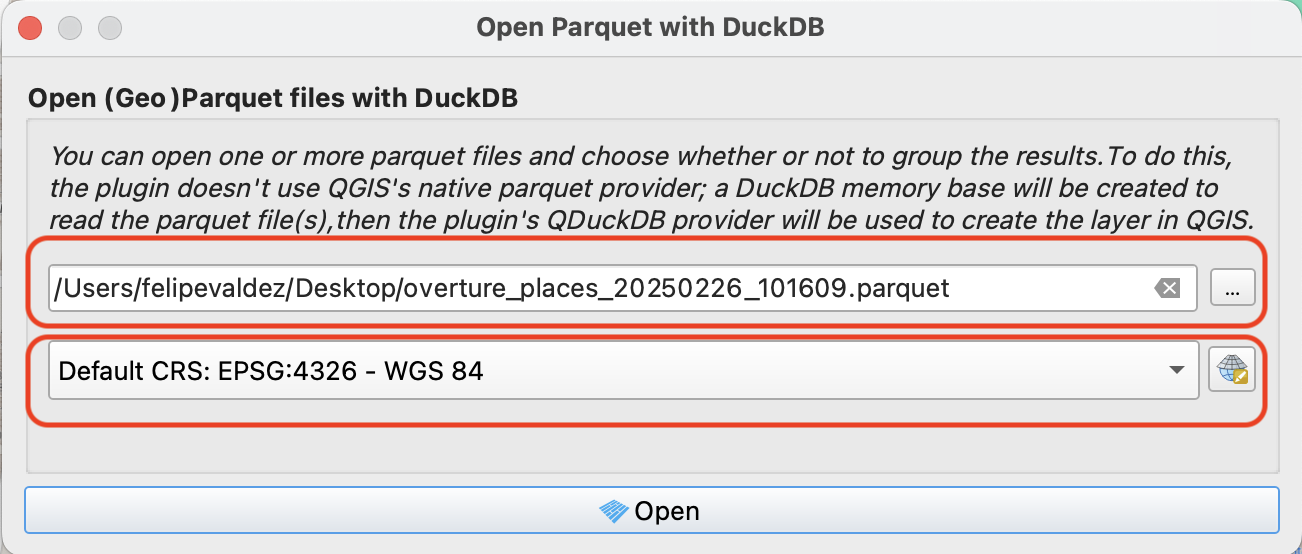
\includegraphics[width=0.7\linewidth,height=\textheight,keepaspectratio]{./images/duckdb_set.png}

The resulting map shows all places around Temple University downloaded
from Overture Maps

\pandocbounded{\includegraphics[keepaspectratio]{./images/final.png}}

\section*{Attribution}\label{attribution}
\addcontentsline{toc}{section}{Attribution}

Open Geospatial Data by Felipe Valdez is licensed under CC BY-NC-SA 4.0




\end{document}
